%%%%%%%%%%%%%%%%%%%%%%%%%%%%%%%%%%%%%%%%%
% OIST Doctoral Thesis - Final bound version
% LaTeX Template
% Version 0.2 (2016/04/06)
%
% This version is the final binding version which will be published.
%
% Original author:
% Jeremie Gillet
%
%%%%%%%%%%%%%%%%%%%%%%%%%%%%%%%%%%%%%%%%%

%----------------------------------------------------------------------------------------
%	PACKAGES AND OTHER DOCUMENT CONFIGURATIONS
%----------------------------------------------------------------------------------------

\documentclass[12pt, twoside]{book} % 12 pt font, two-sided book style
\usepackage[a4paper, includehead, headheight=0.6cm, inner=3cm ,outer=2.5cm, top=2.5 cm, bottom=2.5cm]{geometry}  % Changing size of document
\usepackage[english]{babel} % The document is in English
\usepackage[utf8]{inputenc} % UTF8 encoding
\usepackage[T1]{fontenc} % Font encoding

\usepackage{graphicx} % For including images
\graphicspath{{./Images/}} % Specifies the directory where pictures are stored

\usepackage{longtable} % tables that can span several pages
\usepackage[bf]{caption} % caption: FIG in bold
\usepackage{fancyhdr} % For the headers

\newcommand{\numberedchapter}{ % Preparation for numbered chapters
	\cleardoublepage % To make sure the previous headers are passed
	\fancyhead[RE]{{\bfseries \leftmark}}% Headers for left pages
	\fancyhead[LO]{{\bfseries \rightmark}}}% Headers for right pages
\newcommand{\unnumberedchapter}[1]{ % Preparation for unnumbered chapters
	\cleardoublepage % To make sure the previous headers are passed
	\addcontentsline{toc}{chapter}{#1} % Also adds the chapter name to the Contents
	\fancyhead[RE]{{\bfseries #1}} % Headers for left pages
	\fancyhead[LO]{}}%Headers for right pages

\usepackage{emptypage} % No headers on an empty page

\usepackage{eso-pic} % For the background picture on the title page
\newcommand\BackgroundPic{%
\put(-250,-140){%
\parbox[b][\paperheight]{\paperwidth}{%
\vfill
\centering

\includegraphics[width=\paperwidth]{symbol.jpg}%
\vfill
}}}

\usepackage{hyperref} % Adds clickable links at references

%----------------------------------------------------------------------------------------
%	ADD YOUR CUSTOM VALUES, COMMANDS AND PACKAGES
%----------------------------------------------------------------------------------------

% Open Preamble/mydefinitions.tex and enter some values (name, thesis title...)
% and include your own custom LaTeX functions and packages

%----------------------------------------------------------------------------------------
%	VALUES FOR THE THESIS
%----------------------------------------------------------------------------------------

\newcommand{\name}{Lee James O'Riordan} % Author name
%\newcommand{\thesistitle}{The life and death of vortex 161} % Title of the thesis
\newcommand{\thesistitle}{Non-equilibrium vortex dynamics in rapidly rotating Bose--Einstein condensates} % Title of the thesis
\newcommand{\submissiondate}{October, 2016} % Submission date "Month, year"
\newcommand{\supervisor}{Prof. Thomas Busch} % Supervisor name
%\newcommand{\cosupervisor}{C.~O'Supervisor} % Co-Supervisor name, comment this line if there is none


%----------------------------------------------------------------------------------------
%	BIBLIOGRAPHY STYLE (pick the style you want)
%----------------------------------------------------------------------------------------

\usepackage[square, numbers, sort&compress]{natbib} % for bibliography - Square brackets, citing references with numbers, citations sorted by appearance in the text and compressed (as in [4-7])
%\usepackage[longnamesfirst,round]{natbib} % Natural Sciences bibliography

\bibliographystyle{Preamble/url} % You may use a different style adapted to your field
%\bibliographystyle{unsrtnat} % You may use a different style adapted to your field
%\bibliographystyle{Preamble/mlxd} % You may use a different style adapted to your field


%----------------------------------------------------------------------------------------
%	YOUR PACKAGES (be careful of package interaction)
%----------------------------------------------------------------------------------------


\usepackage{amsthm,amsmath,amssymb,amsfonts,bbm}% Math symbols
\usepackage{flexisym,mathrsfs,cancel}
\usepackage[parfill]{parskip}
%\usepackage{tocbibind}
\PassOptionsToPackage{hyphens}{url}\usepackage{hyperref}
%\usepackage[hyphens]{url}

\usepackage{chapterbib}
\usepackage{float}


%\iffalse
%%%%%%% For stopping figures taking their own pages
\setcounter{topnumber}{2}
\setcounter{bottomnumber}{2}
\setcounter{totalnumber}{4}
\renewcommand{\topfraction}{0.85}
\renewcommand{\bottomfraction}{0.85}
\renewcommand{\textfraction}{0.15}
\renewcommand{\floatpagefraction}{0.8}
\renewcommand{\textfraction}{0.1}
\setlength{\floatsep}{10pt plus 3pt minus 3pt}
\setlength{\textfloatsep}{3ex plus 1pt minus 1pt}
\setlength{\intextsep}{10pt plus 3pt minus 3pt}

\setlength{\belowcaptionskip}{3ex plus 1pt minus 1pt}
%%%%%%%
%\fi

%DOOM

\newfontfamily\doomfontL[Path=./fonts/]{AmazDooMLeft.ttf}
\newfontfamily\doomfontR[Path=./fonts/]{AmazDooMRight.ttf}
\newfontfamily\doomfontLO[Path=./fonts/]{AmazDooMLeftOutline.ttf}

%%%

\DeclareMathOperator*{\atantwo}{atan2}
\DeclareMathOperator*{\argmin}{arg\,min}

%\DeclareMathOperator*{\textprime}{'}

\newcommand{\lee}{\textcolor{red}}
\usepackage{todonotes}
\usepackage{subcaption}
\usepackage{braket} %useful to type directly diacritic characters
\usepackage{algpseudocode}
%\usepackage{xeCJK}
%\setCJKmainfont{MS Mincho} % for \rmfamily
%\setCJKsansfont{MS Gothic} % for \sffamily
%\usepackage{unicode-math}
%\setmathfont{xits-math.otf}


%\usepackage[utf8]{inputenc}
%----------------------------------------------------------------------------------------
%	YOUR DEFINITIONS AND COMMANDS
%----------------------------------------------------------------------------------------

% New Commands
    \renewcommand{\baselinestretch}{1.2}


\newcommand{\bea}{\begin{eqnarray}} % Shortcut for equation arrays
\newcommand{\eea}{\end{eqnarray}}
\newcommand{\e}[1]{\times 10^{#1}}  % Powers of 10 notation

% Defining a theorem box for Criteria
\newtheorem{critere}{Criterion}
\newcommand{\crit}[2]{
\begin{center}
\fbox{ \begin{minipage}[c]{0.9 \textwidth}
\begin{critere}
\textbf{\textup{ #1}} --- #2
\end{critere}
\end{minipage}  } \end{center}
}


\begin{document}

%----------------------------------------------------------------------------------------
%	TITLE PAGE
%----------------------------------------------------------------------------------------

\pagestyle{empty} % No page numbers
\frontmatter % Use roman page numbering style (i, ii, iii, iv...) for the preamble pages

\begin{titlepage}
\AddToShipoutPicture*{\BackgroundPic}
\begin{center}
\vfill
{\large \scshape Okinawa Institute of Science and Technology\\Graduate University}\\[0.7cm]
{\large Thesis submitted for the degree }\\[0.7cm]
{\Large Doctor of Philosophy}\\[0.5cm]
\rule{\textwidth}{1.5pt}\\[0.5cm]
{\huge \bfseries \thesistitle}\\[0.5cm]
\rule{\textwidth}{1.5pt}\\[2.5cm]
\hfill  by\\[1cm]
\hfill  {\large \bfseries\name}\\
\vfill
{\hfill \large Supervisor: \textbf{\supervisor}} \\
\ifx\cosupervisor\undefined\else{\hfill \large Co-Supervisor: \textbf{\cosupervisor}} \\ \fi
\vspace{1cm}
\hfill  \submissiondate
\end{center}
\end{titlepage}

%----------------------------------------------------------------------------------------
%	PREAMBLE PAGES (comment out unnecessary pages)
%----------------------------------------------------------------------------------------

\pagestyle{fancy} % Changes the headers
\renewcommand{\chaptermark}[1]{ \markboth{#1}{}} % Getting the chapter name right
\renewcommand{\sectionmark}[1]{\markright{\thesection\; #1}} % Getting the section name right
\fancyhf{}% Clears header and footer
\fancyhead[RO,LE]{\thepage} % page number on the outside of headers

\unnumberedchapter{Declaration of Original and Sole Authorship} 
\chapter*{Declaration of Original and Sole Authorship} 

I, \name, declare that this thesis entitled \emph{\thesistitle} and the data presented in it are original and my own work. 


I confirm that:
\begin{itemize}
\item This work was done solely while a candidate for the research degree at the Okinawa Institute of Science and Technology Graduate University, Japan.
\item No part of this work has previously been submitted for a degree at this or any other university.
\item References to the work of others have been clearly attributed. Quotations from the work of others have been clearly indicated, and attributed to them.
\item In cases where others have contributed to part of this work, such contribution has been clearly acknowledged and distinguished from my own work.
\item None of this work has been previously published elsewhere, with the exception of the following: (provide list of publications or presentations, or delete this part). 
(If the work of any co-authors appears in this thesis, authorization such as a release or signed waiver from all affected co-authors must be obtained prior to publishing the thesis.  If so, attach copies of this authorization to your initial and final submitted versions, as a separate document for retention by the Graduate School, and indicate on this page that such authorization has been obtained).  
\end{itemize}

Date:  \submissiondate

Signature: 

\unnumberedchapter{Abstract}
\chapter*{Abstract}
\subsection*{\thesistitle}

This body of work examines the non-equilibrium dynamics of vortex lattice carrying Bose--Einstein condensates. We solve the mean-field Gross--Pitaevskii equation for a two-dimensional pancake geometry, in the co-rotating frame within the limit of high rotation frequencies. The condensate responds to this by creating a large periodic lattice of vortices with 6-fold triangular symmetry. By applying two distinct perturbations to this lattice, we examine the resulting effects on the vortices during time evolution. The first perturbation involves applying an optical potential with matching geometry to the vortex lattice. We observe the appearance of interference fringes, and we show that these can be described by moir\'e interference theory. This is backed up by a decomposition of the kinetic energy spectra of the condensate. The applied perturbation only modifies the condensate density, with the vortex positions largely unaffected. From this we conclude that the vortex lattice is very stable and robust against phononic disturbances.

Next, by removing vortices at predefined positions in the lattice using phase imprinting techniques, we examine the resulting order of the lattice. By performing this we generate stable topological defects in the crystal structure.  The resulting lattice remains highly ordered in the presence of low numbers of these defects, where crystal structure and order of the lattice shows to be highly robust. By varying the type of imprinted phases we can create controllable degrees of disorder in the lattice. This disorder is analysed using orientational correlations, Delaunay triangulation, and Voronoi diagrams of the vortex lattice, and demonstrates a method for examining order and generating disorder in vortex lattices in Bose--Einstein condensates.

All work described makes extensive use of GPU computing techniques, and allows for the simulation of these systems to be realised in short times. The implementation of the calculations using GPU computing are also discussed, where the software is shown to be the fastest of its kind out of the independently tested software suites. 

\unnumberedchapter{Acknowledgment}
\chapter*{Acknowledgments}

%\begin{figure}[h!]\centering
%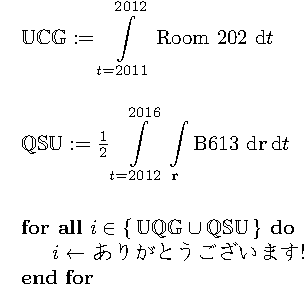
\includegraphics[width=0.4\textwidth]{Preamble/ack_stand/ack_stand}
%\vspace{1ex}
%\end{figure}
%\begin{lstlisting}[breaklines]
$/*$
Firstly, I would like to express my sincerest gratitude to my family back in the 'mel who have always been there for me, and provided amazing support from across the planet since I started my PhD (and before I started too) --- most notably, to Mum, Nan and Maria, who have done so much over the years. Next, my sincerest gratitude and thanks goes to Prof. Thomas Busch, for freeing me from the shackles of a boring job and introducing me to the (ultra)cool world of atomic physics, as well as the guidance he has offered over the years. To past and present members of both the Ultracold Quantum Gases group at University College Cork, and Quantum Systems Unit at OIST, thanks for keeping me sane and helping out through the work and writing over the years --- in no particular order: Mossy, Steve, Jeremie, Tara, Albert, Angela, Sawako, Rashi, James, Irina, the magnificent Dave Rea, and of course Tadhg. Next, I would like to thank the Graduate School for all of their help removing bureaucratic dealings from my everyday life here. A special thanks also goes to the Scientific Computing Section, for allowing me access to some very amazing toys over these past few years. A special thanks also to Annie, for supplying me with enough caffeine to get to the moon and back. Lastly, but not least-ly, to Christina for her compassion, understanding, and assistance over the past few years. $*/$
%\end{lstlisting}


\begin{algorithmic}
\ForAll{$i \in \{S | S \in \textrm{People to thank} \}$}
    \State $i\gets$ ありがとうございます!
\EndFor
\end{algorithmic}

\unnumberedchapter{Abbreviations} 
\chapter*{Abbreviations} 

All abbreviations used in the thesis should be listed here, with their definitions, in alphabetical order.  This includes trivial and commonly used abbreviations (at your own discretion), but not words that have entered into general English usage (such as laser or DNA).  In particular, non-standard abbreviations should be presented here.  This is an aid to the reader who may not read all sections of the thesis. \\ % You can delete this paragraph, only the table is needed.

\begin{longtable}{rl}
PPT & positive partial transpose\\
SRPT & Schr\"odinger-Robertson partial transpose
\end{longtable}
\unnumberedchapter{Glossary} 
\chapter*{Glossary} 

% Break up this table into several ones if it takes up more than one page
\begin{center}
\begin{longtable}{r p{0.58 \textwidth}}
Chemical potential & Energy to overcome for adding an atom to the system
\end{longtable}
\end{center}

\unnumberedchapter{Nomenclature} 
\chapter*{Nomenclature} 

% Break up this table into several ones if it takes up more than one page
\begin{longtable}{rl}
$h$ & Planck constant ($6.626\ 070\ 04\e{-34}\ \mbox{Js}$). \\
$\hbar$ & Planck constant over $2\pi$ ($1.054\ 572\ 66\e{-34}\ \mbox{Js}$). \\
$L_z$ & Angular momentum operator along the $z$-dimension; $xp_y-yp_x$. \\
$\nabla$ & Gradient operator. \\
$\Omega$ & Angular rotation frequency of condensate. \\
$\xi$ & Condensate healing length; the distance from a region of zero density at vortex core to bulk density. \\
$\mu$ & Chemical potential of the condensate; the energy change per unit change in particle number. \\
\end{longtable}
\cleardoublepage
\thispagestyle{empty} % Page style needs to be empty for this page

\vspace*{8cm} 

\hfill
\begin{parbox}{0.6\textwidth}{
\begin{flushright}

If desired, an optional and short dedication may be included here.

\end{flushright}}
\end{parbox}




%----------------------------------------------------------------------------------------
%	LIST OF CONTENTS/FIGURES/TABLES
%----------------------------------------------------------------------------------------

\unnumberedchapter{Contents}
\tableofcontents % Write out the Table of Contents
\unnumberedchapter{List of Figures}
\listoffigures % Write out the List of Figures
\unnumberedchapter{List of Tables}
\listoftables % Write out the List of Tables

%----------------------------------------------------------------------------------------
%	THESIS MAIN TEXT - CHAPTERS
%----------------------------------------------------------------------------------------

\addtocontents{toc}{\vspace{2em}} % Add a gap in the Contents, for aesthetics
\mainmatter % Begin numeric (1,2,3...) page numbering

\unnumberedchapter{Introduction} % Title of the unnumbered chapter
%\chapter*{Introduction}  % Name of the unnumbered section

This body of work was carried out during my time as a Ph.D student at Okinawa Institute of Science and Technology Graduate University (OIST). The purpose of the work described herein was to understand the dynamics of rapidly rotating Bose--Einstein condensates subjected to perturbations. While it is possible derive some analytical solutions to rapidly rotating condensate behaviour (LLL), such solutions are rare. This thesis concentrates on the numerical solutions of the Gross--Pitaevskii equation, and the resulting dynamics of those solutions.

This work is motivated by the use of Bose--Einstein condensate (BEC) systems as model tools to investigate turbulent and chaotic quantum behaviour. Ideally, these systems can also be used for long-term memory storage for quantum computing systems. Finally, these type of systems allow the study of quantum mechanical effects on mesoscopic scales, making them a great tool for simulating condensed matter physics. Given these statements, being able to manipulate and engineer specific states, and thus behaviour, from BECs requires tools to allow this. I investigate the use of kicked optical potentials and direct phase engineering of the wavefunction and examine their usefulness for generating such behaviour.

To do this we assume a trial system of a BEC rapidly rotating to generate a large number of vortices, arranged in a triangular pattern pattern. The trial wavefunction is subjected to the different manipulations listed earlier, and I examine the resulting dynamics. A large numerical component will be required to perform such simulations, and so I will also discuss the development of numerical tools using graphics processing units (GPU) for these studies, with comparisons drawn against standard simulation techniques.

The thesis will be outlined as follows:

\section{Chapter 1}
The field of cold-atomic gas systems will be introduced, and the theory of Bose--Einstein condensation discussed. The field will be thoroughly examined and discussed via a literature review, examining theory, experimentation, origins and also future of the field. Emphasis will be placed on material and works relevant to the study performed herein.

\iffalse
Introduction (~5-10 pages)

    - Thesis Statement (one or two sentences)
        What is your thesis about and what have you done?
        If you have a hypothesis what is it?
        How will you test (prove/disprove) your hypothesis?
    - Motivation
        Why is this problem you've worked on important
    - Goals / Objectives
        What are you trying to do and why?
        How will you or the reader know if or when you've met your objectives?
    - **** Contributions *****
        What is new, different, better, significant?
        Why is the world a better place because of what you've done?
        What have you contributed to the field of research?
        What is now known/possible/better because of your thesis?
    Outline of the thesis (optional)
\fi

\section{Chapter 2}
    Here I examine the use of methods for describing the Bose--Einstein condensate numerically. I introduce the necessary algorithms and considerations to simulate such a system. General purpose GPU (GPGPU) computing will be introduced here, with the implementation of the Gross--Pitaevskii equation discussed. Calculation of the Bogoloiubov spectrum, and its implementation is discussed here also.

\iffalse
Background / Related Work (~8-20 pages)
    More than a literature review
    Organize related work - impose structure
    Be clear as to how previous work being described relates to your own.
    The reader should not be left wondering why you've described something!!
    Critique the existing work - Where is it strong where is it weak? What are the unreasonable/undesirable assumptions?
    Identify opportunities for more research (i.e., your thesis) Are there unaddressed, or more important related topics?
    After reading this chapter, one should understand the motivation for and importance of your thesis
    You should clearly and precisely define all of the key concepts dealt with in the rest of the thesis, and teach the reader what s/he needs to know to understand the rest of the thesis.
\fi

\section{Chapter 3}
\iffalse
Theory / Solution / Program / Problem (~15-30 pages)

    continuing from Chapter 2 explain the issues
    outline your solution / extension / refutation
\fi

\section{Chapter 4}

\iffalse Implementation / Formalism (~15-30 pages)
    not every thesis has or needs an implementation
\fi

\section{Chapter 5}

\iffalse
Results and Evaluation (~15-30 pages)

    adequacy, efficiency, productiveness, effectiveness (choose your criteria, state them clearly and justify them)
    be careful that you are using a fair measure, and that you are actually measuring what you claim to be measuring
    if comparing with previous techniques those techniques must be described in Chapter 2
    be honest in evaluation
    admit weaknesses
\fi

\section{Chapter 6}
\iffalse
 Conclusions and Future Work (~5-10 pages)

    State what you've done and what you've found
    Summarize contributions (achievements and impact)
    Outline open issues/directions for future work
\fi
 % Introduction (unnumbered)

\numberedchapter
%%%%%%%%%%%%%%%%%%%%%%%%%%%%%%%%%%%%%%
\newif\iflitrev
\iflitrev
    \chapter{Literature review}
        In this document I review the area of cold atomic gases, and in particular the superfluid behaviour of Bose--Einstein condensate systems. The history of this area will be discussed, highlighting both theoretical and experimental observations. With the fundamentals of Bose--Einstein condensation explained, I will then examine the dynamical behaviour of condensates from the perspective of superfluidity. Vortex behaviour will be discussed, along with recent results, concentrating on the dynamics of vortices in response to external potentials.

 Following this, quantum chaos will be introduced, along with the many of the interesting dynamics that can be observed in superfluid flow. The creation and observation of quantum chaotic dynamics in a Bose--Einstein condensate shall be proposed. The goal of the proposed project will be to generate chaotic dynamics using a vortex lattice subjected to a periodically pulsed optical lattice. Beginning with a well defined state, generation of chaotic behaviour shall be examined. The Hamiltonian required to generate a vortex lattice in a condensate shall be mapped to the delta-kicked harmonic oscillator Hamiltonian, which will provide a model system to understand the observed system dynamics. To characterise the resulting dynamics, the trajectories of the vortices shall be plotted over the course of the evolution of the system. Further information may be obtained by examining the system using phase--space methods and Floquet theory to characterise the observed behaviours. Experiments to observe chaotic behaviour in the quantum regime are rare, and the realisation of this type of system should allow for the first of its kind to observe chaos in a system of well-ordered topological excitations. Given recent experimental progress in the area of trapping, cooling, rotating and controlling Bose--Einstein condensates, the proposed system should be realisable with currently available experimental techniques.
 % Import your chapters here
        \section{Cold atoms}
\subsection{Cooling of atomic gases}\label{sub:cooling}
One of the major advances in experimental physics in recent times has been the laser cooling of trapped atoms to temperatures near absolute zero. This feat, which garnered the Nobel Prize in Physics in 1997, resulted from the pioneering work of C. Cohen-Tannoudji, S. Chu and W. Phillips \cite{AO:Chu_revmod_1998,AO:Cohen_revmod_1998,AO:Phillips_revmod_1998}. It relies on the use of counter-propagating detuned laser fields which are directed upon a trapped cloud of atoms. Due to Doppler shifting of the frequencies, atoms moving towards the respective beams see resonant photons, absorb them and slow down due to the momentum absorbed, with this technique being termed Doppler cooling. This is followed by a spontaneous emission in a random direction, for which the recoil kicks average out to zero. Hence, the atoms become cooler. As a result, the atoms will eventually reach a velocity below that which will cause an absorption from the lasers, leaving a less broad velocity distribution. Although laser cooling allowed temperatures to reach micro-Kelvin regimes, additional techniques must be used to obtain atoms deep in the nano-Kelvin temperature range. One such method, known as evaporative cooling, involves relaxation of the trapping potential height, which in turn allows many of the higher energy atoms to escape \cite{AO:Ketterle_amop_1996}. The remaining atoms rethermalise and are thus of lower energy, and therefore at a lower temperature. With these techniques the creation of Bose--Einstein condensates in dilute atomic gases became possible.

\subsection{Introduction to Bose--Einstein condensation}\label{sub:becintro}
Bose--Einstein condensation was theoretically predicted by N. Bose and A. Einstein \cite{BEC:Ketterle_revmod_2002}. This began as a work on the statistical behaviour of photons, eventually leading to the derivation of the ``Bose--Einstein distribution'' for an ideal bosonic gas.
In the framework of the grand canonical ensemble and following the description given by Pitaevskii and Stringari \cite[chap. 2]{BK:Pitaevskii_Stringari_2003}, the Bose--Einstein distribution is given by
\begin{equation}
\bar{n}_i = \frac{1}{e^{\beta(\epsilon_i - \mu)} -1},
\end{equation}
where $\bar{n}_i$ is the average occupation number of the $i$-th energy state, $\beta=(k_BT)^{-1}$ with $k_B$ being the Boltzmann constant and $T$ as the temperature, $\epsilon_i$ is the $i$-th energy eigenvalue, and $\mu$ is the chemical potential giving the energy required to add an atom to the system.
The total number of particles in the system, $N$, can be evaluated by summing over the individual occupation numbers, as
\begin{equation}
N=\displaystyle\sum_i \bar{n}_i.
\end{equation}
This work predicted that non-interacting, indistinguishable (bosonic) particles would, if their energy was sufficiently low, undergo a phase transition below a critical temperature into a new phase in which the atoms would occupy the same lowest lying energy state of the system. The number of atoms occupying this lowest lying state, $N_0$, is given by the relationship
\begin{equation}
N_0 \equiv \bar{n}_0 = \frac{1}{e^{\beta(\epsilon_0 - \mu)} - 1},
\end{equation}
with $\epsilon_0$ representing the lowest energy eigenvalue. Since negative occupation numbers would be a nonphysical result, the chemical potential is limited to values of $\mu < \epsilon_0$. As $\mu$ tends to $\epsilon_0$ the occupation of the lowest energy state grows large. Separating the total number of atoms into the lowest lying (condensed), $N_0$, and higher lying (thermal), $N_T$, states as
\begin{equation}
N = N_0 + N_T = N_0 + \displaystyle\sum_{i\neq 0}\bar{n}_i(T,\mu),
\end{equation}
a relation for the the onset of Bose--Einstein condensation can be given. This will happen when the temperature drops below a critical value, $T_c$, where $\mu$ will approach $\epsilon_0$, resulting in the macroscopic occupation of the lowest lying state, yielding a Bose--Einstein condensate (BEC).

BECs are a prime example of coherent matter waves, and demonstrate quantum mechanical effects on length-scales which can be considered mesoscopic. Given a cloud of identical bosons at higher temperature, the atoms exhibit billiard-ball type behaviour. As they are cooled, the thermal de Broglie wavelength of the atoms, given by
\begin{equation}
\lambda_{dB} = \sqrt{2\pi\hbar^2/mk_{B}T},
\end{equation}
where $m$ is the atom mass, grows, causes the wave-nature of the atoms to become more prominent, and the atomic waves start to overlap when $\lambda_{dB} \approx$ inter-particle separation. The quantity $n\lambda_{dB}^3$, where $n$ is the density of the gas, is known as the \emph{phase-space density}. Physically this denotes the number of particles present in a box with sides of $\lambda_{dB}$ length, and the phase transition to the condensate sets in at $\zeta\left(\frac{3}{2}\right)$, where $\zeta$ is the Riemann-Zeta function \cite{BK:Ueda_2010}. The value of $T_c$ for this to occur in a uniform gas is given by
\begin{equation}
k_BT_C = \frac{2\pi}{\zeta\left(\frac{3}{2}\right)^{2/3}}\frac{\hbar^2n^{2/3}}{m},
\end{equation}
or, in the case of a harmonic oscillator potential,
\begin{equation}
k_BT_C = \frac{\hbar\bar{\omega}N^{1/3}}{\zeta(3)^{1/3}},
\end{equation}
where $\bar{\omega}=(\omega_x\omega_y\omega_z)^{1/3}$ is the geometric mean of the oscillator frequencies. Critical temperatures for harmonically trapped gases are on the order of nano-Kelvin assuming realisable trapping frequencies, which were experimentally inaccessible during the time of Bose and Einstein.

Fritz London, in 1938, following on from the body of work derived by Einstein and Bose drew the connection between superfluidity in liquid $^4$He and Bose--Einstein condensation \cite[Chap.~1]{BK:Pitaevskii_Stringari_2003}. However, due to the liquid nature of $^4$He at low temperatures only approximately $10\%$ of the atoms condense into a BEC \cite{BEC:Penrose_pr_1956}. In order to achieve the large occupation of the lowest energy state the system must be prepared so that the interparticle interaction strength does not destroy the coherence, as is the case for liquid $^4$He.

Due to their weak interactions, dilute atomic gases are closer to the ideal case discussed by Bose and Einstein. One negative impact, though, were the higher masses of the atoms used in such systems, which required reaching much lower transition temperatures. As such, the use of lighter elements were considered. Spin-polarised hydrogen
was one of the first systems to be investigated to create BEC \cite{BEC:Kleppner_enfe_1998,BK:Pitaevskii_Stringari_2003} in the 1970's. Using trapping and cooling techniques
present at the time, this type of system came close, but did not quite reach the required temperatures and phase-space densities for
Bose--Einstein condensation to occur until over twenty years later \cite{BEC:Fried_prl_1998}. Given the advent of laser cooling in the 1980's, the use of alkali atoms was considered partly due to the ease of accessibility of their optical transition frequencies. It was not until 1995 that the first BECs would be experimentally realised \cite{BEC:Cornell_science_1995,BEC:Ketterle_prl_1995}.

\subsection{Theoretical description of BECs: Gross--Pitaevskii equation}\label{sub:gpederiv}
I will, in the following section, outline the derivation of the mean-field Gross--Pitaevskii equation, which is widely used to study the behaviour of the condensate in many works cited in this review. Following the \textit{Les Houches 2013 Lecture Course} by J. Walraven \cite{LEC:Walraven_lh_2013} the second quantization form of the many-body Hamiltonian for interacting particles in a harmonic potential is given by
\begin{equation}\label{eqn:ham2ndq}
\hat{\mathcal{H}} = \hat{H_1} + \hat{H_2} = \int \hat{\Psi}^{\dagger} H_0\left(\textbf{r},\textbf{p} \right)  \hat{\Psi} \; d\textbf{r}  + \frac{1}{2} \int\hat{\Psi}^{\dagger}\hat{\Psi}^{\dagger}V_{\textrm{int}}(\textbf{r}^\prime-\textbf{r})\hat{\Psi}\hat{\Psi} \; d\textbf{r}^\prime d\textbf{r},
\end{equation}
with $H_0\left(\textbf{r}, \textbf{p} \right) = -\frac{\hbar}{2m}\nabla^2 + V_{\textrm{ext}}\left(\textbf{r}\right)$. The external potential, $V_{\text{ext}}(r)$ is taken as harmonic, of the form
\begin{equation}
V_{\text{ext}}(\textbf{r}) = \frac{m}{2}\displaystyle\sum_{i}{\omega_i r_i},
\end{equation}
and with $\omega_i$ representing the trapping frequency in the $i$-th spatial dimension. The interaction potential, $V_{\text{int}}$ is assumed to be point-like as
\begin{equation}\label{eqn:v_int}
	V_{\text{int}}\left(\textbf{r}_i,\textbf{r}_j \right) = g\delta\left(\textbf{r}_i - \textbf{r}_j\right),
\end{equation} where $\delta$ is the Dirac delta function and the mean-field interaction, $g$ is given by
\begin{equation}
	g = \frac{4\pi\hbar^2 a_s}{m},
\end{equation}
with $a_s$ being the s-wave scattering length. Inserting the contact potential Eq. \eqref{eqn:v_int} into the second quantised interaction Hamiltonian $\hat{H}_2$ from Eq. \eqref{eqn:ham2ndq} above yields the following relations
\begin{align}
\hat{H}_2 &= \frac{g}{2} \int \hat{\Psi}^{\dagger}(\textbf{r})\hat{\Psi}^{\dagger}(\textbf{r\textprime}) \delta\left(\textbf{r} - \textbf{r\textprime}\right)\hat{\Psi}(\textbf{r\textprime})\hat{\Psi}(\textbf{r})d\textbf{r}d\textbf{r\textprime} \\
 & = \frac{g}{2}\int \hat{\Psi}^{\dagger}(\textbf{r})\hat{\Psi}^{\dagger}(\textbf{r}) \hat{\Psi}(\textbf{r})\hat{\Psi}(\textbf{r})d\textbf{r}d\textbf{r} \\
 & = \frac{g}{2}\int \hat{\Psi}^{\dagger}\left(\textbf{r}\right)\hat{n}\left(\textbf{\textbf{r}}\right)\hat{\Psi}^{\dagger}d\textbf{r}.
\end{align}
In the Heisenberg picture, the evolution of the system is governed by the equation
\begin{equation}\label{eqn:heisenberg}
i\hbar \frac{\partial}{\partial t}\hat{\Psi}_H\left(\textbf{r}, t\right) = \left[\hat{\Psi}_{H}\left(\textbf{r}, t\right), \hat{\mathcal{H}}  \right],
\end{equation}
where the Heisenberg field annihilation operator, $\hat{\Psi}_H\left(\textbf{r}, t\right)$, is given by
\begin{equation}\label{eqn:psi_heisenberg}
\hat{\Psi}_H\left(\textbf{r}, {t} \right) = e^{\frac{i\hat{\mathcal{H}}t}{\hbar}}\hat{\Psi}\left(\textbf{r}\right) e^{\frac{-i\hat{\mathcal{H}}t}{\hbar}}.
\end{equation}
The operator, $\hat{\Psi}_H$ can be interpreted as the one removing an atom from a given state of the system. Therefore, if all $N$ atoms in the system are in the ground-state, $\vert 0_N\rangle$, as would be the case in an ideal condensate, the following relationship holds
\begin{align}
\hat{\Psi}_{H}(\textbf{r},t)\vert 0_N \rangle &= e^{\frac{iE_0(N-1)t}{\hbar}}\hat{\Psi}(\textbf{r})e^{\frac{-iE_0(N)t}{\hbar}}\vert 0_N \rangle \\
&= \hat{\Psi}(\textbf{r})e^{\frac{i[E_0(N-1) - E_0(N)]t}{\hbar}} \vert 0_N \rangle \\
&= \hat{\Psi}(\textbf{r})e^{\frac{-i\mu t}{\hbar}} \vert 0_N \rangle, \label{eqn:stationary_soln}
\end{align}
where $\mu=E_0(N) - E_0(N-1)$ is the chemical potential. Using the bosonic commutation relations
\begin{eqnarray}
\left[\hat{\Psi}(\textbf{r}'), \hat{\Psi}^{\dagger}(\textbf{r})\right] &=& \delta(\textbf{r}' - \textbf{r}), \\
\left[\hat{\Psi}(\textbf{r}'), \hat{\Psi}(\textbf{r})\right] &=& \left[\hat{\Psi}^{\dagger}(\textbf{r}'), \hat{\Psi}^{\dagger}(\textbf{r})\right] = 0,
\end{eqnarray}
and noting the following relations
\begin{align}
\left[\hat{\Psi}(\textbf{r}),\hat{H}_1 \right] & = \hat{H}_0(\textbf{r},\textbf{p})\hat{\Psi}(\textbf{r}), \\
\left[\hat{\Psi}(\textbf{r}),\hat{H}_2 \right] & = g\hat{n}(\textbf{r})\hat{\Psi}(\textbf{r}), \\
\left[\hat{\Psi}(\textbf{r}),\hat{n} \right] & = \hat{\Psi}(\textbf{r}) ,
\end{align}
the Hamiltonian Eq. \eqref{eqn:ham2ndq} can be rewritten in the following form
\begin{equation}\label{eqn:h_many}
\mathcal{H} = \displaystyle\sum\limits_{i=1}^N \left( -\frac{\hbar^2}{2m}\nabla^2  + V(\textbf{r}_i)\right) + \frac{1}{2}g\displaystyle\sum\limits_{i\neq j}\delta(\textbf{r}_i - \textbf{r}_j).
\end{equation}
Due to the macroscopic occupation of the lowest lying single-particle state, $\hat{\Psi}$ can be treated as a classical field, $\Psi$, neglecting all quantum fluctuations involving higher-lying states. Substituting Eq. \eqref{eqn:h_many} and \eqref{eqn:psi_heisenberg} into \eqref{eqn:heisenberg}, the time dependent mean-field Gross--Pitaevskii equation (GPE) can then be written as
\begin{equation}\label{eqn:gpe}
i\hbar\frac{\partial}{\partial t}\Psi(\textbf{r},t) = \left[-\frac{\hbar^2}{2m}\nabla^2 + V(\textbf{r}) + g\vert\Psi(\textbf{r},t)\vert^2 \right]\Psi(\textbf{r},t).
\end{equation}
The time independent form can be found by substituting Eq. \eqref{eqn:stationary_soln} into \eqref{eqn:gpe}, yielding
\begin{equation}
\mu\Psi(\textbf{r}) = \left[-\frac{\hbar^2}{2m}\nabla^2 + V(\textbf{r}) + g\vert\Psi(\textbf{r},t)\vert^2 \right]\Psi(\textbf{r}),
\end{equation}
where the wavefunction is normalised to the particle number, $N$, as follows
\begin{equation}\label{eqn:norm}
\displaystyle\int\limits_{-\infty}^{\infty}d\textbf{r} \left\vert \Psi\left(\textbf{r}\right) \right\vert^2 = N.
\end{equation}
In the case of a rotating condensate an additional term appears in the GPE, $-\Omega L$, where $\Omega$ is the angular rotation frequency, and $L$ is the angular momentum. Assuming rotation about a single axis, the longitudinal direction, $z$, $L$ can be replaced with $L_z$, giving the final form of the GPE in the co-rotating frame as
\begin{equation}\label{eqn:gpe_rotation}
i\hbar\frac{\partial}{\partial t}\Psi(\textbf{r},t) = \left[-\frac{\hbar^2}{2m}\nabla^2 + V(\textbf{r}) + g\vert\Psi(\textbf{r},t)\vert^2 - \Omega L_z  \right]\Psi(\textbf{r},t).
\end{equation}
This mean-field equation can be used to describe the behaviour of the condensate, provided the number of atoms is sufficiently large ($>10^3$ for most experimental set-ups) and the correlations are not too strong. Assuming a large number of bosons in the condensate, $N$, the interaction term dominates over the kinetic term of the Hamiltonian which can therefore be neglected. This turns finding the ground-state of the system into a solvable, algebraic problem, and is known as the Thomas-Fermi approximation \cite[~p. 84]{BK:Ueda_2010}. The Hamiltonian can thus be reduced to a combination of the trapping potential and the mean-field interaction, and the wavefunction, $\psi_{\textrm{TF}}$, can be determined from the time independent GPE as
\begin{equation}
\psi_{TF}(\textbf{r}) = \sqrt{ g^{-1}[\mu - V(\textbf{r})] \Theta(\mu - V(\textbf{r}))},
\end{equation}
where $\mu$ is the chemical potential, and $\Theta$ is the Heaviside step function, which ensures that the condensate density does not become negative. Within this regime the condensate can be described by hydrodynamical equations \cite[Pg.~180]{BK:Pitaevskii_Stringari_2003}, and from this, an approximate value for the cloud radius can be determined, called the Thomas-Fermi radius. The boundary of the cloud is determined by the surface at which the density becomes zero, and corresponds to the point where the trapping potential and chemical potential are equivalent. This gives the geometric mean spatial extent of the cloud \cite[~p. 169]{BK:Pethick_Smith_2008} as
\begin{equation}
\bar{R} = \left(\frac{15Na}{\bar{a}}\right)^{1/5}\bar{a},
\end{equation}
where the characteristic length of the harmonic oscillator is given by
$\bar{a} = \sqrt{{\hbar}/{m\bar{\omega}}}$. Thus, within the Thomas-Fermi radius, it is possible to explain the behaviour of the BEC analytically and compare with exact numerical results from integrating the full GPE.

\subsection{Realisation of Bose--Einstein condensation in dilute gases}\label{sub:becdev}
Following the first experimental realisations of a BEC in dilute atomic gases by E. Cornell and C. Wiemann at University of Colorado, Boulder \cite{BEC:Cornell_science_1995}, and W. Ketterle at M.I.T. \cite{BEC:Ketterle_prl_1995}, work was carried out by Baym and Pethick \cite{BEC:Baym_prl_1996}, who investigated the mean-field ground-state solution in the Thomas-Fermi limit of a magnetically trapped rubidium BEC, as was created in the Boulder experiment.
%Learning from the techniques used and developed for condensation of alkali atoms, the group of D.~Kleppner and T.~Greytak succeeded in developing a condensate of spin-polarised hydrogen \cite{Fried_prl_1998}, following a twenty-year experimental search.

In a first comprehensive review of the area only a few years later by Dalfovo \textit{et al}. \cite{BEC:Dalfovo_revmod_1999}, the underlying theory of trapped Bose--Einstein condensates was examined in detail. The review discusses how the combination of laser cooling and evaporative cooling \cite{AO:Ketterle_amop_1996} allowed the experimentalists to reach the temperatures and required phase-space densities for Bose--Einstein condensation to occur. Ground-state properties of the system are examined assuming an effective interaction. Stationary properties of harmonically trapped condensates are discussed, in the framework of mean-field theory (Gross--Pitaevskii), which is shown to allow for the determination of system properties and dynamics. Attractive versus repulsive interactions are examined, followed by a discussion of ``Beyond mean-field theory'', where corrections to the theory are applied to enable more exact determination of ground-state energies.

The nature of vortices in a condensate are considered, and in particular critical angular velocities, core size, and imaging. Given the coherence of atoms in a condensate, matter-wave interference by simply expanding and overlapping two condensates is suggested, and the appearance of a dislocation in the interference pattern is a sign of the presence of a vortex. The authors further indicate the accurate agreement of mean-field theory with known experimental data, and differences between observation and mean-field predictions are mentioned. %Due to the level of complexity involved in obtaining a condensate, a significant degree of work is performed on developing a solid theoretical understanding of dynamical behaviour under many differing conditions.

Interpenetrating condensates are discussed in a paper by Sinatra \textit{et al}. \cite{BEC:Sinatra_prl_1999}, where the authors present a theoretical prediction of the mixing of a two-component, initially separated condensate. Predicted oscillations of the mean condensate separation were compared to the Boulder (JILA) experiment, and showed good agreement, supporting the use of mean-field theory in predicting condensate dynamics.

\subsection{Lower dimensional condensates}\label{sub:coldatom_recent}
Another area of interest in BEC systems is that of low-dimensional condensates, such as the work undertaken by G\"{o}rlitz \textit{et al}. \cite{BEC:Gorlitz_prl_2001}, wherein a strong axial confinement of the
condensate in the $z$-dimension is used to effectively create a ``pancake'' condensate in an optical trap. This trapping geometry restricts motion in the axial direction, creating effective two-dimensional dynamics. This may be extended further to one-dimension by using elongated ``cigar'' traps via magnetic potentials, such as those existing on atom-chip structures \cite{AO:Denschlag_prl_1999,AO:Folman_prl_2000,AO:Haase_pra_2001}, or in optical potentials. G\"{o}rlitz \textit{et al.} state that in lower dimensional systems phenomena such as solitons and vortices should have much greater stability, and should therefore be more suitable for investigating them. Realisation of a Tonks-Girardeau gas is also discussed, with such systems becoming accessible using optical potentials such as described by Moritz \textit{et al}. \cite{OL:Moritz_prl_2003}. Work in the effective 2D regime is of particular interest, and condensate behaviour in relation to excitations has been examined under such conditions. Kimura \cite{BEC:Kimura_pra_2002} investigates the dynamical behaviour of condensate breathing modes in both two and one dimensions. Tanatar \textit{et al}. \cite{BEC:Tanatar_arxiv_2002} consider the use of a tightly-confined pancake condensate, and discuss differences occurring to the inter-atomic scattering as a function of confinement strength along the $z$-dimension. Both mentioned works consider use of the Thomas--Fermi approximation, comparing results obtained analytically with that of numerical integration using the Gross--Pitaevskii equation.

%In the following section, I will discuss the condensate behaviour from the perspective of a superfluid, as superfluidity is an inherent property of a gaseous BEC. This will be approached using a GPE formalism.
 % Import your chapters here
        \section{Superfluidity}\label{sec:superfluid}
\subsection{Introduction to superfluidity}
A classical fluid in a rotating vessel will eventually reach a steady-state wherein the fluid rotates as a whole with the container as a solid-body. This behaviour emerges as a result of the viscosity of the fluid and, assuming the no-slip condition \cite{FL:Day_2010}, that the fluid elements in direct contact with the boundary of the container adhere to its surface. Given sufficient time to reach equilibrium, the entire fluid will rotate at the same angular velocity. If the driving forces are removed, this flow will eventually cease to rotate, and once again become stationary. Such flow can be contrasted with that of an inviscid flow, and will not experience any effect from the boundary rotation. Once in motion, an inviscid fluid will continue to rotate indefinitely. This type of flow can be realised with superfluids \cite{BK:Prandtl_2010}.

Superfluidity is a macroscopic quantum effect that is closely related to Bose--Einstein condensation. Liquid helium has been known for many years to exhibit this superfluid behaviour \cite{BEC:Penrose_pr_1956}. One interesting property of superfluids is that they have quantized circulation which can lead to the appearance of quantum vortices under rotation. Traditionally, such excitations have been created in liquid $^4$He by a ``rotating bucket'' type of experiment, where the container is rotated about a single axis. When the fluid is initially above the $\lambda$-critical point, the temperature at which $^4$He moves from a classical fluid to a superfluid, the atoms will undergo solid-body rotation with the container. On cooling the atoms below the $\lambda$-critical point liquid $^4$He will undergo a transition to the superfluid state. If the velocity is above a critical rotation value vortices are nucleated in the rotating superfluid helium system. Due to the strongly interacting nature of liquid helium the nucleated vortices are difficult to visualise as the healing length, $\xi$, of liquid $^4$He, the length over which the central zero density core of a vortex increases to the superfluid bulk density, is on the order of {\r{A}}ngstr{\"o}ms \cite{BEC:Srinivasen_pramana_2006}.

In order to visualise such vortices experimentally it was necessary to use an indirect means of visualisation in the form of tracer particles \cite{BEC:Packard_physb_1982}. Limited success was had with this technique using solid hydrogen, and later plastic microspheres, as they tended to join together due to static charges. An improved technique, using charged particles, showed much greater success \cite{Vtx:Packard_prl_1969}. Ions, or electrons, were trapped inside the vortex lines, and an electric field along the direction of the lines allowed for acceleration of the charges towards a luminescent screen where they could be observed. Current experimental work in vortex visualisation with liquid $^4$He has advanced significantly \cite{Vtx:Tsubota_arxiv_2010,Vtx:Guo_pnas_2014}, yet fine control over the behaviour of the liquid and the vortex dynamics remains difficult.

Superfluid behaviour is observed in liquid helium due partly to a portion of the atoms condensing into the ground-state. Given that BECs show superfluidity, the use of a dilute gas where the majority of atoms are in the condensate state provides a more controlled means to investigate superfluidity and quantised vortices \cite{BK:Ueda_2010,BEC:Srinivasen_pramana_2006,Vtx:Tsubota_arxiv_2010,CT:Tsubota_jpsj_2008}. In contrast with liquid $^4$He, having a healing length of the order of nanometers, the healing length of a dilute gas of alkali atoms is on the order of microns \cite{Vtx:Isoshima_pra_1999}. This places condensates in a much more accessible regime for visualising vortices compared with liquid $^4$He experiments. To fully understand the behaviour of the system, it is necessary to have a framework for modelling the condensate, in the absence and the presence of vortices. A dilute gas of condensed atoms close to absolute zero temperature can be readily modelled by the Gross--Pitaevskii equation \eqref{eqn:gpe_rotation}, offering a direct means to simulate condensate behaviour. It is useful to obtain a hydrodynamic description for the condensate, performed by treating its wave-function as
\begin{equation}\label{eqn:madelung}
\Psi(\textbf{r},t) = \vert\Psi(\textbf{r},t)\vert e^{i\theta(\textbf{r},t)},
\end{equation}
where $\theta(\textbf{r},t)$ is the condensate phase, and $\vert\Psi(\textbf{r},t)\vert=\sqrt{\rho(\textbf{r},t)}$, the square root of the condensate density \cite[~chap. 1]{BK:Pitaevskii_Stringari_2003}.
The formalism used below follows that given by Ueda \cite{BK:Ueda_2010}, where the condensate density is given by
\begin{equation}\label{eqn:density}
\rho(\textbf{r},t) = \Psi^*(\textbf{r},t)\Psi(\textbf{r},t) = \vert \Psi (\textbf{r},t) \vert ^2.
\end{equation}
The continuity relation takes the form
\begin{equation}\label{eqn:continuity}
\frac{\partial}{\partial t}\rho(\textbf{r},t)  + \nabla \textbf{j}(\textbf{r},t) = 0,
\end{equation}
where the current density of the condensate is
\begin{equation}\label{eqn:current_density}
\textbf{j}(\textbf{r},t) = \frac{-i\hbar}{2m}\left[\Psi^*(\textbf{r},t)\nabla\Psi(\textbf{r},t) - \Psi(\textbf{r},t)\nabla\Psi^*(\textbf{r},t)\right].
\end{equation}
Using ansatz \eqref{eqn:madelung} and substituting it into Eq. \eqref{eqn:current_density} then gives the form for the current density,
\begin{equation}
\textbf{j}(\textbf{r},t) = \vert\Psi(\textbf{r},t)\vert ^2\frac{\hbar}{m}\nabla\theta(\textbf{r},t).
\end{equation}
The velocity of the superfluid, $\textbf{v}(\textbf{r},t)$ is defined as the ratio of the current density to the density, and then is given by
\begin{equation}\label{eqn:velocity}
\textbf{v}(\textbf{r},t)\equiv \frac{\textbf{j}(\textbf{r},t)}{\rho(\textbf{r},t)} = \frac{\hbar}{m}\nabla\theta(\textbf{r},t).
\end{equation}
The gradient of the phase therefore gives the velocity of the condensate atoms; this indicates that the superfluid behaviour in a condensate is irrotational ($\nabla\times(\nabla\theta) =0$). Assuming a closed loop integral about a central point in the condensate, and recalling the single-valued nature of the wavefunction, yields the relationship
\begin{equation}\label{eqn:circulation}
\oint_C \textbf{v}\cdot d\textbf{l} = \frac{\hbar}{m}2\pi l.
\end{equation}
This shows the quantised nature of circulation in a superfluid, with $l$ representing the integer charge of the circulation. The phase winding around the central region is given by multiples of $2\pi$, with the centre of the phase becoming ill-defined. To circumvent this problem the density at this point drops to zero, signalling the presence of a vortex in the condensate density. This drop happens over the scale of the healing length, which, for repulsive interactions, is given by
\begin{equation}
\xi = \frac{1}{\sqrt{8\pi \rho a_s}},
\end{equation}
where $\rho$ is the bulk density of the condensate, and $a_s$ is the s-wave scattering length.
To sustain a vortex the condensate must have sufficient angular momentum, which is imparted via the angular momentum term $-\Omega L_z$
in the Hamiltonian given by Eq. \eqref{eqn:gpe_rotation}. This term accounts for rotation of the condensate, and puts us in the co-rotating
frame. The angular velocity, $\Omega$, of the condensate has an upper-bound stability limit equivalent to the transverse trapping frequency, $\omega_{\perp}$, of the harmonically trapped condensate.

I will now further discuss both theory and experimental results for vortex behaviour in condensate systems.

\subsection{Vortices in Bose--Einstein condensates}\label{ss:vorticesinbec}
In \cite{BEC:Stringari_prl_1996} Stringari derives equations for the moment of inertia for the condensate, and shows that above $T_c$ the moment of inertia can be described classically. Below $T_c$ the moment of inertia is represented as a sum of two terms, one describing the classical solid-body rotation of the thermal cloud, the other describing the irrotational flow of the condensed cloud.  At zero Kelvin, the moment of inertia is given entirely by the irrotational component, indicating that all atoms are condensed.

A paper by Dalfovo and Stringari \cite{Vtx:Dalfovo_pra_1996} suggested the possibility of exciting vortices using an anisotropy in the
trapping potential. The authors discuss the applicability of mean-field Gross--Pitaevskii theory to a such problem. An examination into the behaviour of vortex flow is given and the solutions for the ground-state and vortex carrying states are found via numerical minimisation of the Gross--Pitaevskii energy functional. A decrease in the critical angular velocity for vortex formation with an increase in the number of condensate atoms, $N$, is shown. For attractive interactions, the critical angular velocity increases with larger $N$. Ground-state results are compared to experimental data from the JILA (Boulder) experiment \cite{BEC:Cornell_science_1995}, and were found to be in good agreement. A closely related work is one by Barenghi \cite{Vtx:Barenghi_pra_1996}, who discusses finite temperature corrections to the zero temperature regime to account for displacements of the vortex cores. It shows how small thermal excitations can, even at low temperatures, affect the vortex position. The work of Lundh \textit{et al}. \cite{Vtx:Lundh_pra_1997} further extends that of Dalfovo and Stringari. Here, the authors investigate the lowest required angular velocity that allows a vortex to enter a condensate, and consider corrections to the Thomas--Fermi approximation. They discuss the use of both isotropic and anisotropic trapping geometries, and find good agreement between the numerical integration of the GPE for experimentally realistic parameters, and analytical expressions they derive for the kinetic energy and the lower-bound on the critical angular velocity for a vortex to enter the atomic cloud.

Marzlin \textit{et al}. \cite{Vtx:Marzlin_prl_1997} proposed a different method for generating vortex states. They consider a condensate subjected to two Laguerre--Gaussian beams of $\sigma^+$ and $\sigma^-$ polarisation respectively. The beams are chosen to be resonant with an internal transition, and transfer angular momentum through the coupling allowing the condensate to start rotating. Another method, investigated numerically by Jackson \textit{et al}. \cite{Vtx:Jackson_prl_1998} uses a blue-detuned light field to simulate an object moving through an effective two-dimensional BEC, which can be achieved by tightly confining it in the $z$-direction. They show the formation of vortices close to the centre of the laser potential, whose movement causes a ``phase-slip'', with the value of the phase going from $-\pi$ to $\pi$ around the vortex. They also note that the speed of vortex shedding from the object has an inverse relationship to the speed of sound in the condensate, given as
\begin{equation}
c(\textbf{r},t) = \sqrt{\frac{\rho (\textbf{r},t) U}{m}},
\end{equation}
where $U=4\pi\hbar^2 a_s/m$ represents the repulsive atom-atom interaction \cite{BEC:Andrews_prl_1997}. A second paper by Marzlin \textit{et al}. \cite{Vtx:Zhang_pra_1998} suggests the use of an optical dipole potential resulting from four travelling-wave beams to excite a trapped condensate and induce circulation by transfer of angular momentum. Results of this study show that for harmonic trapping potentials a superposition of vortex states is created. Pure vortex states are shown to arise only from anharmonic traps combined with a rotating linear potential. This topic is treated by the same authors in a follow up work \cite{Vtx:Marzlin_pra_1998}.

Building upon the earlier discussion by Marzlin \textit{et al}., Goldstein \textit{et al}. \cite{Vtx:Goldstein_pra_1998} consider schemes for accurate detection of the topological charge of a trapped condensate containing vortices. Their idea builds on the interference of the vortex carrying condensate with a second ground-state condensate, and they show that the vanishing of interference lines is related to the vortex charge. A work provided by Svidzinsky \textit{et al}. \cite{Vtx:Svidzinsky_pra_1998} discusses the hydrodynamic formalism within the Thomas-Fermi limit, and show it is an effective means of describing condensate behaviour in the presence of vortices. An alternative approach is presented by Lundh \textit{et al}. \cite{Vtx:Lundh_pra_1998}, who consider methods for vortex detection methods in large condensates. They discuss the difficulties that arise when only a single vortex is present, as the energy difference to the vortex-less ground state would be too small to measure. They consider the free expansion of both a two and three-dimensional condensate, which allows a singly charged vortex core to expand as well and become visible on an absorption picture. They note that in two-dimensions (2D) the vortex core and condensate expand at roughly the same rate, making detection somewhat more challenging than in three-dimensions (3D) where the core initially expands faster than the condensate. Lundh \textit{et al}. also note that in the limit of weak coupling a difference exists between the aspect ratios of condensates with and without vortices, and that this effect is enhanced by anisotropic trapping geometries.

The stability of vortex states in a condensate is also a widely discussed topic \cite{Vtx:Fedichev_pra_1999,Vtx:Feder_prl_1999}, as non-rotating traps show an instability for small displacements of the vortex from the trap centre. However, Feder \textit{et al}. \cite{Vtx:Feder_prl_1999} calculated the critical rotation frequencies for vortex stabilisation at the centre of an anharmonic rotating trap. Further proposed schemes to realise vortex carrying condensates are given by the following theoretical works \cite{Vtx:Anglin_prl_1999,Vtx:Davies_prl_1999,Vtx:Marshall_pra_1999,Vtx:Dobrek_pra_1999}. The method proposed by Dobrek \textit{et al}. \cite{Vtx:Dobrek_pra_1999}, shows a means to optically generate vortices by the use of what they term a ``phase-imprinting'' method. The authors describe a scheme where
the phase of the condensate is controlled directly, and given the required topological charge to induce a vortex during evolution. Through use of an absorption plate whose axis angle depends on the absorption coefficient, the condensate can be imprinted with the required phase pattern.

The realisation of vortices in a two-component condensate was first achieved by Matthews \textit{et al}. \cite{Vtx:Matthews_prl_1999}. Using two internal states of $^{87}$Rb, the authors coherently coupled and induced transitions between both in such a way that one component acquired a $2\pi$ phase winding and rotated around the other component. A different route to creating vortices was successfully used by Madison \textit{et al}. \cite{Vtx:Madison_prl_2000}, who tightly focused a laser to stir the condensate beyond a critical frequency for nucleation. This way they were able to generate multiple vortices in the condensate.

\subsection{Vortex lattices}
In early 1999, Castin and Dum \cite{Vtx:Castin_epjd_1999} examined the ground-state solutions for multi-vortex condensates, simulating up to 18 vortices. Their work is mostly performed in effective 2D, with data for a 3D configuration given following the main body of work. At the same time Feder \textit{et al}. \cite{Vtx:Feder_pra_2000} considered the case where multiple vortices are present in the condensate, and performed a numerical investigation of this on a 3D condensate of $^{23}$Na. The authors further mention that given a sufficient number of vortices in the condensate an almost regular triangular array would be observed. Evidence for this behaviour could be seen in the experimental data obtained by Madison \textit{et al}. \cite{Vtx:Madison_jmo_2000}, showing up to 11 vortices that seemingly arrange in a triangular array pattern. This resulted from laser stirring of the condensate, and was also covered in \cite{Vtx:Madison_prl_2000}. A follow-up study by Madison \textit{et al}. \cite{Vtx:Madison_prl_2001}, and Chevy \textit{et al}. \cite{Vtx:Chevy_aoi_2001} showed the relationship between vortex nucleation and the dynamical instabilities arising from the irrotational state, specifically, the excitation of the rotating quadrupolar mode of the condensate.

%Another method to realise vortices in a BEC is provided by Ogawa \textit{et al}. \cite{Vtx:Ogawa_pra_2002}. They proposed using spinor BEC in an Ioffe-Pritchard trap with a hyperfine $\vert F=1 \vert$ state. Through adiabatic variation of an axially applied magnetic field, $B_z$, a phase winding of $4\pi$ can be generated via manipulation of the spin degrees of freedom. An ``optical plug'', which is a blue-detuned laser field, was used along the vortex core to prevent atom losses due to Majorana spin flips when $\vert B \vert = 0$. The authors state that the process through which the phase accumulates a winding can be understood as a Berry phase during the evolution of the spins. The resulting vortex generated via this means is unstable due to the larger winding, and such will decay into singly charged vortices. Following the procedure given previously by Ogawa \textit{et al}., a theoretical analysis was performed by M\"ott\"onen \textit{et al}. \cite{Vtx:Mottonen_jpcm_2002} on vortex generation in a condensate with a hyperfine $\vert F=2 \vert$ state, showing the generation of a vortex with a phase winding of $8\pi$. This is reported to remain stable only in the presence of an optical plug, decaying into 4 singly charged vortices otherwise.

Of all the work on multiple vortex generation and the underlying theory, one of the seminal works of the time was the experiment from Ketterle's group on vortex lattices \cite{Vtx:AboShaeer_sci_2001}. The authors begin with a comparison of vortices to the type of behaviour observed in type--II superconductors, where penetration of the magnetic field into the conductor is possible only via quantised flux lines. They then state that ``(v)orticity can enter rotating superfluids only in the form of discrete line defects with quantized circulation'', and therefore establish a close connection between the rotational properties of superfluids and superconductors. Furthermore, their experiment finds Abrikosov (triangular) style vortex lattices, which are also known from type--II superconductors. The group generated condensates with lattices containing upwards of 130 vortices, in a well ordered triangular formation. This was achieved through stirring of the condensate with a blue-detuned laser which was moved symmetrically around the condensate at a specified angular frequency, $\Omega$. The conclusions drawn by the authors are that BECs are a robust system for generating vortex lattice structures that naturally form into a regular triangular pattern, and show many similarities to type--II superconductors.

Ho \cite{Vtx:Ho_prl_2001} showed that the behaviour observed in the fast rotation limit closely resembles that of the two-dimensional quantum Hall regime, where the system is residing in the lowest Landau level, $LLL$ ($n=0$). Ho states that the experimental data suggests the MIT group has not yet reached the LLL regime, but are very close. As the rotation of the cloud approaches the trapping frequency, the system tends to the LLL. However, in this regime the Thomas--Fermi approximation becomes invalid, requiring a more accurate consideration of the $z$-components. He concludes by stating that rotation close to the trap frequency will require treatment beyond that of the mean-field approach. An additional study from the MIT group \cite{Vtx:Raman_prl_2001} derived a result showing that the number of vortices in the condensate is proportional to the rotational frequency of the stirrer at a given frequency. They discuss the cause of vortex nucleation as a consequence of surfaces modes in the condensate and due to localised regions of turbulent behaviour.

The group at JILA devised a method to systematically evaporatively cool and rotate a cloud of $^{87}$Rb confined in a harmonic potential \cite{Vtx:Haljan_prl_2001}. Beginning with a normal fluid component close to $T_c$, the harmonic trapping potential is initially deformed and rotated. This induces a rotation of the cloud, until it enters a solid-body rotational state with the trap. Upon
reaching a steady-state, the rotating asymmetry is switched off, and the cloud is evaporatively cooled. This approach is similar to that of the rotating bucket experiment in liquid $^4$He. By applying an additional distortion to the trapping geometry allows for the removal of atoms with large axial displacements to take place, and as a result of this, the temperature of the cloud is reduced by a factor of four. Additionally, the rotation rate of the remaining cloud increases as the angular momentum per particle stays close to constant. At the end of the evaporation process, a condensate forms at the centre of the cloud, rotating with a frequency as high as 0.94 times the confining potential frequency. Results are compared with the theoretical calculations of Feder and Clark \cite{Vtx:Feder_prl_2001}, and were stated to agree.

Although a large number of works exist which investigate systems with low numbers of vortices \cite{THS:Davies_2000,Vtx:Chevy_prl_2000,Vtx:Cooper_prl_2001,Vtx:Rosenbusch_prl_2002,Vtx:Ogawa_pra_2002,Vtx:Bretin_joptb_2003}, I will concentrate primarily on studies of systems containing a large number of vortices. Engels \textit{et al}. \cite{Vtx:Engels_prl_2002} were capable of creating condensates containing equivalent numbers of vortices to those obtained in the MIT experiments, and investigated the behaviour of these lattices with respect to excitation of higher lying modes. The authors show a ``sheetlike structure'' of the condensate vortices in the presence of an $m_z=-2$ surface mode. It is discussed that due to the difficulty in obtaining dense vortex lattices in pancake-like condensates that this may provide a means to investigate such behaviour.
%without the need to consider then experimentally inaccessible rotation rates and low atom numbers.

Adhikari \textit{et al}. \cite{BEC:Adhikari_pra_2002} carried out numerical simulations of condensate behaviour subjected to a sudden perturbation of the trapping potential. The authors discuss changes in the interaction strength, the trapping potential, and the rotation of the condensate, and how a vortex will decay once rotation has ceased. Their simulations considered quasi (effective) two-dimensional condensates and solved the GPE using a split-operator technique \cite{BEC:Javanainen_jphysa_2006}. Subjected to a perturbation pulse the condensate boundary starts to oscillate, and the number of supported vortices changes dependent upon the sign of interaction change or trapping potential.

\subsection{Fast rotation limit}
Mueller and Ho \cite{Vtx:Mueller_prl_2002} considered the case of a two-component condensate under fast-rotation, above the previously reported rotation rates that were experimentally accessible. Such systems are stated to be in the ``mean-field quantum Hall regime'', where each component can be described by an individual wave-function with an angular momentum large enough to ensure the LLL regime. These systems are a generalisation of the work by Ho \cite{Vtx:Ho_prl_2001}, and the authors show that the minimum energy state corresponds to a pair of interspersed vortex lattices, one for each respective component. They also show that variation of the interaction parameters allows the geometric arrangement of the lattices to be be modified, for example into a rhombic structure. An additional theoretical examination of vortices in the quantum Hall regime $(\Omega\approx\omega_{\perp})$ is offered by Subrahmanyam \cite{Vtx:Subrahmanyam_pra_2003}. At such rotation rates the aspect ratio of the condensate, namely the ratio of the width in the $z$-dimension to the width in the $x$--$y$ plane, becomes very small yielding an effective two-dimensional system.
%This is in line with the two-dimensional quantum Hall system, where the number of vortices will be on par with the number of atoms in the condensate, and where the vortex lattice unit cell equals the Larmor circle.
It is also stated that in this limit the use of mean-field theory will fail due to perturbations becoming more prominent, and a full model for interacting bosons becomes necessary to fully describe the dynamics. For rotation rates less than this limit, however, the vortices arrange themselves into the expected triangular lattice. This work in the mean-field quantum Hall (MFQH) regime is further extended by Regnault and Jolicoer \cite{Vtx:Regnault_prl_2003}, who describe fractional quantum Hall (FQH) behaviour in condensate systems by using a non mean-field formalism. For the body of work I describe later, it will be assumed that the rotation rates will remain below FQH regime rotation rates, allowing for a MFQH description.

%In his thesis, Penckwitt \cite{THS:Penckwitt_2003} examines the theoretical formalism behind vortex lattice generation and behaviour in a condensate. Of particular interest is the settling of the lattice into a stable state using a rotating atom cloud. The basis of the investigation is formed from results given by Gardiner \textit{et al}. \cite{BEC:Gardiner_jphysb_2002}, with discussion of and investigation into some of the methods presented from the experimental results available at the time.

Given the known upper limit of the rotational frequency for which a harmonically trapped condensate is stable, which is the harmonic trapping frequency, one might inquire as to whether other configurations exist in which higher rotation rates can be achieved. An investigation performed by Bretin \textit{et al}. \cite{BEC:Bretin_prl_2004} considers a condensate trapped within a quadratic plus quartic (QQ) potential, with an additional theoretical analysis for both the repulsive and attractive interaction cases given by Ghosh \cite{Vtx:Ghosh_pra_2004}.
%Beginning with a mention of all known work on the area, including but not limited to \cite{Vtx:Matthews_prl_1999,Vtx:Madison_prl_2000,Vtx:AboShaeer_sci_2001,Vtx:Haljan_prl_2001,Vtx:Ho_prl_2001,Vtx:Regnault_prl_2003},
Bretin \textit{et al}. examine the behaviour of the system at the limiting point $\Omega=\omega_{\perp}$, stating that the angular momentum of the system
becomes singular. A comparison is made to a charged particle in a magnetic field, with an energy spectrum reminiscent of Landau levels with a $2\hbar\omega$ separation, as stated previously by Mueller and Ho \cite{Vtx:Mueller_prl_2002}. Through inclusion of the additional quartic term, the system can be examined at rotation frequencies at, and slightly beyond, the trapping frequency. Rotation frequencies of up to 0.95$\omega_{\perp}$ are shown to result in regular vortex lattices, with values beyond this inducing distortions to the structure of the lattice. The authors also mention that at rotation frequencies close to the trapping frequencies significant time is required ``to reach a well ordered vortex lattice'' when performing imaginary time evolution to find the system ground-state. The observation of giant vortices, which are possible within this regime, are mentioned but not discussed in much detail.

The creation of such a MFQH system which can be described by the LLL was another milestone for the JILA group, and was reported in a paper by Schweikhard \textit{et al}. \cite{Vtx:Schweikhard_prl_2004}. The authors successfully demonstrate a condensate rotated upwards of 0.99 times $\omega_{\perp}$. Given that this regime displays behaviour different to the known results at the time, the importance of comparing the regime to the well known Thomas--Fermi limit was an important next step. Such a work was carried out by Watanabe \textit{et al}. \cite{Vtx:Watanabe_prl_2004}. They showed that the density profile of the rotating condensate in the MFQH limit was described well by the Thomas--Fermi approximation. This was shown to hold true provided that the number of vortices is much larger than unity, or that the condensate size is large in comparison with the harmonic oscillator length in the transverse direction, $\bar{a}_{\perp} = \sqrt{\hbar/m\omega_{\perp}}$. Comparing the MFQH regime to the Thomas--Fermi limit was also studied by Zhai \textit{et al}. \cite{Vtx:Zhai_pra_2004} who investigated the behaviour of two overlapping vortex lattices.

As mentioned earlier, the Thomas--Fermi limit describes the case where the kinetic energy term of the Hamiltonian may be neglected in comparison to the interaction energy, as it offers little contribution to the condensate behaviour. This remains true for low rotation rates, however kinetic energy becomes important in the limit of fast rotation. In this case $\Omega/\omega_{\perp}\approx 1$, and the centrifugal force term, $m\Omega^2r$, almost balances with the trapping force term, $-m\omega^2r$. The kinetic energy term can no longer be neglected here, but one may now consider the condensate in the MFQH regime. The interaction energy is then much less than the gap between energy levels for single particle Landau levels \cite{Vtx:Ho_prl_2001}. Zhai \textit{et al}. state that the difference between these two regimes are characterised purely by the ratio of the kinetic energy to the interaction energy of the system, and in the MFQH regime we can thus assume the LLL has been achieved.

Assuming the LLL description for a fast rotating Bose--Einstein condensate, the Dalibard group provide many theoretical works using this framework, beginning with the work offered by Aftalion \textit{et al}. \cite{Vtx:Aftalion_pra_2005}. The authors describe the case where the number of
atoms to the number vortices, denoted as the ``filling factor'', $\nu=N/N_v$ \cite{BK:Ueda_2010,Vtx:Ho_prl_2001}, becomes an important characteristic of the system. In the case where the number of vortices is small compared to the number of atoms (still under the fast rotation limit), the system may be accurately described to be in the MFQH regime. However, as the rotational frequency of the condensate approaches the trapping frequency, the condensate width expands, and will tend to infinity. In this limit the number of vortices is comparable to the number of condensate atoms, and the system can no longer be described by a single macroscopic wave-function. Instead it can be described as being similar to ``an electron gas in the fractional quantum Hall regime''. To avoid dealing with the FQH regime, the authors restrict themselves to the MFQH regime, and choose rotational frequencies that guarantee this. The MFQH regime is entered when $1000 > \nu > 10$, which is attained close to the $\Omega / \omega_{\perp}\approx 1$ limit. One of the key conclusions from this paper is that the density distribution of the condensate in the MFQH regime is that of an inverted parabola, with the vortices forming a triangular lattice pattern that is almost regular. The area of each vortex cell differs from that of the solid-body rotating case, and is significantly distorted at the edge of the condensate. The results of Schweikhard \textit{et al}. \cite{Vtx:Schweikhard_prl_2004} are found to agree with what is proposed in this work, but they differ from the findings by Ho \cite{Vtx:Ho_prl_2001}, which predicted a Gaussian density distribution with an infinite regular lattice. For an almost perfectly regular lattice, the rotation rate must be sufficiently large that the condensate width extends to large distances and a large number of vortices are generated, without entering the FQH regime. For such a system, the vortices about the central region will be uniformly ordered due to the balanced velocity fields. Vortices on the condensate edge will have a distorted alignment, and can be neglected.

A closely related work undertaken by Stock \textit{et al}. \cite{BEC:Stock_laserphyslett_2005} offers a brief review of many of the results relevant to vortex behaviour in condensates, up to and beyond the $\Omega=\omega_{\perp}$ regime. They discuss many of the known results in the MFQH regime, analogies to Landau levels, the use of QQ potentials, and briefly the FQH regime. Vibrational modes of vortex lattices, such as the Kelvin and Tkachenko modes, which are oscillations of the vortex line and vortex lattice respectively, are also reviewed. The use of QQ potentials is discussed as a way to allow observation of vortices with winding numbers larger than unity, where a purely quadratic potential would be unstable. Finally, they restate the fact that when the number of vortices approaches the atom number of the condensate, the system will no longer be capably described by a mean-field theory. Instead it enters a strongly correlated regime mirroring that of FQH regime, the observation of which is experimentally possible only for low atom numbers. A similarly comprehensive review of experimental results is offered by Srinivasan \cite{BEC:Srinivasen_pramana_2006}, and covers much of the same material, albeit with greater detail in parts.

%\subsection{Vortices in largely asymmetric potentials}
%Most of the work reviewed previously involved symmetric trapping geometries when discussing the fast rotation regime. The use of asymmetric trapping potentials may prove to have interesting effects on condensate behaviour. An examination of vortex lattice structures in the fast rotation limit is offered by Oktel \cite{Vtx:Oktel_pra_2004} for the 2D trapping potential stretched along one of the dimensions. He showed that the lattice arrangement still favours an Abrikosov triangular structure, and states that this is within an experimentally accessible parameter range. If we consider equating the lowest trapping frequencies with the rotation frequency how will the system behave? Two papers investigating this problem are that of Sinha \textit{et al}. \cite{Vtx:Sinha_prl_2005}, and Sanchez-Lotero \textit{et al}. \cite{Vtx:Lotero_pra_2005}, and both demonstrate a similar finding: when the rotation rate approaches that of the lower trap frequency the condensate extends along the more loosely confined dimension, and becomes ``free'' when the frequencies are equal. A quantum channel forms as a result, with the vortices aligning in rows. However, with an increase in interaction strength between bosons in the condensate, the triangular vortex lattice can be recovered. Sinha \textit{et al}. mention that, similar to the symmetric case, the mean-field treatment fails as the vortex number approaches that of the atom number. The authors do discuss that, given a proper treatment accounting for quantum fluctuations, the obtained lattice is expected to melt in this limit. Further similarities between the symmetric and asymmetric trapping geometries are drawn by Fetter \cite{Vtx:Fetter_pra_2007}, who considers a 2D condensate at rotation rates approaching the lesser of the trap frequencies. Both systems can be modelled using a LLL wavefunction approach, however pointing out that it is not clear if ``this situation holds for arbitrary anisotropy and less extreme rotation speeds''. Fetter also mentions the transition to the quantum channel regime, suggesting that a correlated state may be involved in this transition, leaving it open for further investigation. Aftalion \textit{et al}. \cite{Vtx:Aftalion_pra_2009} show that for the case of fast rotation in asymmetric trapping geometries the condensate is expected to not display any vortices in the bulk density. With minor anisotropy the condensate will have a Thomas--Fermi profile in the LLL description similar to the isotropic case, and also showing lattice distortion on the condensate edges as previously reported. In the fast rotation regime, however, the condensate bulk remains free of visible vortices, with no lattice forming. The resulting density profile shows an inverted parabola in the unconfined ($\Omega = \omega_i$) dimension, with a Gaussian profile in the other dimension. This behaviour has similarities to the condensate in a QQ potential, wherein the bulk density shows no vortices at high rotation, a result shown by Fetter \textit{et al}. \cite{Vtx:Fetter_pra_2005}. They conclude by stating that beginning with a resting condensate and subjecting it to high rotation in this regime should not nucleate any vortices.

%Filling the void between slow \cite{Vtx:Oktel_pra_2004} and fast rotation \cite{Vtx:Aftalion_pra_2009}, the work of McEndoo \textit{et al}. \cite{Vtx:McEndoo_pra_2009} investigates the anisotropic regime for moderate rotation speeds, and hence low vortex numbers. The vortex lattice structure is shown to transition from the triangular lattice to that of a linear chain. The authors also discover that the critical stirring frequency of the condensate to nucleate a vortex increases for larger anisotropies in 2D. The role of symmetry during vortex nucleation at various rotation rates was examined by Dagnino \textit{et al}. \cite{Vtx:Dagnino_natphys_2009}, who investigated changes in the system symmetry over a sweeping of the rotation rate of the condensate, $\Omega$. The nucleation of a single vortex into the condensate for a given rotation rate is a symmetry--breaking process, and close to the critical symmetry breaking value, $\Omega_c$, the system fails to be described accurately by mean-field theory, which is appropriate at values above and below this transition point. The system is expected to exhibit strongly correlated behaviour at the critical values, and the paper discusses the limitations of the mean-field approach around this point. This indicates that to use a mean-field approach, the system parameters must be carefully chosen so that the system remains stable and away from the symmetry breaking points. The study concludes by discussing a formalism for describing quantum modes that may be investigated using Bogoliubov--de Gennes theory, stating that it agrees well with the full theory. The authors also restate the problem as a ``requantization'' of the mean-field theory into single particle states, originally described by Parke \textit{et al}. \cite{Vtx:Parke_prl_2008} as a means to describe effects outside the mean-field approach, even at low rotational frequencies.

Given the wealth of literature available on rotating condensates, a review of all experimental and theoretical results then available was compiled and published by Fetter \cite{BEC:Fetter_revmodphys_2009}. The author draws some conclusions and defines a future outlook for the field.
\begin{itemize}
\item Theory and experiment agree well for rotational frequencies reaching approximately $0.995\omega_{\perp}$.\vspace{-1em}
\item The density profile of slowly rotating condensates differs very little from that of non-rotating condensates, except for the inclusion of the vortex cores.\vspace{-1em}
\item The Thomas--Fermi regime holds true for frequencies of $0.75 \leq \Omega \leq 0.99$, where kinetic energy remains negligible compared to flow velocity.\vspace{-1em}
\item The MFQH regime LLL description, holding for $0.99 \leq \Omega \leq 0.999$, sees the vortex cores expanding to fill all available condensate space. Density variation gives rise to energy terms of the order of flow velocity.
\end{itemize}
Following these statements, Fetter outlines some goals to observe effects and behaviours predicted to occur in rotating ultracold gas systems that still exist. Approaching and examining the behaviour of a condensate in the fractional quantum Hall regime, wherein $\nu$ is small, remains to be demonstrated. Rapidly rotating Fermi--gases are discussed also as an area requiring future investigation, and which may also provide insight into low $\nu$ states and behaviours.

\subsection{Optical lattice potentials}\label{sub:optlatt}
Trapping potentials for Bose--Einstein condensates are typically harmonic, and are formed using magnetic (such as Ioffe--Pritchard) or optical potentials (such as dipole traps). Although these traps provide a single trapping location for all the atoms, interesting behaviour can also be observed and investigated using of an array of traps. One method of achieving this is the use of counter-propagating laser fields, allowing for a periodic optical potential to be created. For two sets of counter-propagating laser fields in a plane at right angles, an array of one-dimensional cigar-shaped condensate traps can be created, wherein the atoms are tightly confined in 2D. Adding an additional set of fields perpendicular to the existing ones will allow trapping of the atoms to periodic locations corresponding to a cubic lattice \cite[~chap. 2]{BK:LH_2010}. %To model bosonic atoms sitting in an optical potential, the Bose--Hubbard Hamiltonian can be considered \cite{BEC:Bloch_revmodphys_2008}. This model accounts for atoms hopping between nearest neighbour sites on the lattice and also includes the presence of an interaction term,
%\begin{equation}\label{eqn:bosehubbard}
%\hat{H}_{BH} = -J \displaystyle\sum\limits_{<i,j>} \left(\hat{a}_i^\dagger \hat{a}_j + \hat{a}_j^\dagger \hat{a}_i \right) + \frac{U}{2}\displaystyle\sum\limits_i \hat{n}_i(\hat{n}_i - 1).
%\end{equation}
%One of the main features of atoms in optical lattices is that they can be tuned to move between the mean field and the strongly correlated regime \cite{THS:McEndoo_2010}. %In this model the system must be assumed to be subjected to the optical lattice on timescales that allow for it to come to equilibrium within the lattice sites. For the work proposed later in Section \ref{sec:prelim}, this model may not be useful initially as the timescales of application are much shorter than those required to allow the system to reach equilibrium. It may become a necessary part of explaining some system behaviour and dynamics in both referenced and proposed future work, and it is thus valuable to discuss it here. Due to the vast amount of available literature I will concentrate on a much smaller subset of research in this area.

In 2002, the first realisation of a condensate trapped in a three-dimensional optical lattice was achieved by Greiner \textit{et al}. \cite{OL:Greiner_nat_2002}. They successfully realised an optical lattice in which the depth of the individual lattice sites could be adjusted by the intensity of the laser fields. By increasing the intensity from zero allows each site to obtain a number of condensate atoms. The authors show that increasing the intensity of the lattice lasers allows the system to move from a long-range phase coherent (BEC) state, to one where the phases between individual sites are no longer coherent, the so-called Mott insulator state. Such a system can no longer be described by a mean-field theory, and requires the use of a discrete quantum treatment, offered by the Bose--Hubbard model. To ensure the system remains in the ground-state, the intensity of the lattice potential was ramped to the required value slowly compared to the timescales for the system to react. This ensured that no higher modes were excited, and allowed the condensate atoms to distribute amongst the trapping potential.

A theoretical investigation into the effect of optical lattices on vortex lattice structures was undertaken by Reijnders and Duine \cite{OL:Reijnders_prl_2004}. The authors were able to show that for in the presence of an optical potential which is not matched to the vortex lattice the vortices would break from an Abrikosov pattern, and become pinned to optical lattice sites. This was experimentally verified by Tung \textit{et al}. \cite{Vtx:Tung_prl_2006}. They begin by comparing and contrasting pinned and Abrikosov vortex systems, and find that both allow ``correlated many-body states'' to be investigated. They consider competition between both lattice structures, and investigate the resulting behaviour of the condensate. Taking a 2D optical lattice superimposed upon the condensate in the fast rotation limit, the maxima of the optical potential create regions wherein it is energetically favourable for a vortex to sit. The authors show that a vortex may be pinned to a position given by the optical lattice, and through variation of the optical intensity a structural transition can occur from the triangular Abrikosov lattice to that of the optical lattice pattern. This is favoured when the two lattices rotate at the same rate, allowing the lattices to effectively ``lock''. Using this technique the authors demonstrated a square lattice structure.

The use of optical lattices in combination with Bose--Einstein condensates in the manner described previously allows for many interesting effects unique to such systems. One such interesting body of theoretical work was that of S{\o}rensen \textit{et al}. \cite{OL:Sorensen_prl_2005}, which involved the creation of FQH states, in a manner different from the fast-rotation route. The authors describe a process starting with a condensate in a harmonic potential in the Mott insulator state, going to the FQH state via the application of a magnetic field and reduction of the optical lattice potential, where the resulting state is in the LLL. A related work by Palmer \textit{et al}. \cite{OL:Palmer_prl_2006} investigates cold bosons in an optical lattice in the presence of large magnetic fields. The authors show that it is possible to generate FQH states, with varying fractional values. However, the proposed method is rather complex, and is described as requiring near future experimental technology to generate and observe such structures.

Another body of work investigating such behaviour was carried out by Vignolo \textit{et al}. \cite{Vtx:Vignolo_pra_2007}. They investigate vortex dynamics in a condensate upon excitation by a 2D optical lattice. This theoretical study restricts itself to a single vortex, and can therefore be considered realisable using current state of the art technology \cite{Vtx:Matthews_prl_1999,Vtx:Dobrek_pra_1999,Vtx:Tung_prl_2006}. Assuming a zero-temperature Bose gas, and a Bose--Hubbard Hamiltonian description, the authors derive a means of determining a vortex mass of the resulting system. This mass is stated as being easily tunable through variation of the confining potential along the rotation axis, assuming a pancake-shaped condensate. The use of Feshbach resonances \cite{BEC:Chin_revmod_2010} is also mentioned as a possible tool for altering the scattering length of the atoms, which provides a knob for the vortex mass to be adjusted. Through the use of Bragg scattering spectroscopic techniques, the authors state that in the presence of a vortex, the optical lattice structure exhibits a resonance allowing measurement of the vortex mass, which is absent when no vortex is present. The paper concludes by mentioning possible further studies, such as the case wherein interaction and tunnelling strengths are of the same order, or when many vortices are present within the system. These are stated to give rise to more complex system dynamics, and are, in the authors opinions, experimentally realisable.

\subsection{Recent advances and discoveries}
There has been a significant amount of literature examining condensates with and without rotation and/or optical lattices, with both experimental and theoretical progress continuing in this area. The group of G. Campbell \cite{Vtx:Wright_pra_2013} examine the behaviour of a condensate in an annular trapping geometry, which is stirred by an optical potential barrier of varying intensity. Beginning with a stationary condensate, stirring was performed at a fixed rotational velocity using a repulsive potential barrier with diameter less than the trapping annulus width. Using the Thomas--Fermi approximation allowed for estimates of the chemical potential, $\mu$, which in turn determined a value for the trap width and barrier width. Starting from zero intensity, the barrier was ramped to a maximum intensity over 100 ms, remained there for 800 ms and decreased over 100 ms. Following a time-of-flight expansion, excitations of the condensate were observed. Release of a non-rotating condensate shows the central hole of the condensate to close, resulting in a large peak at the centre. In contrast, a circulating condensate will show the presence of one or more holes, which signify ``the presence of phase singularities (vortices)''. If a central hole is observed in the condensate density, the authors state that this is resulting from the presence of persistent currents in the condensate, which prior to release were flowing around the annular trap. The resulting diameter of the hole is dependent upon the winding number of the circulating current in the condensate. Holes that were reported as being off-centre show the presence of topological excitations (vortices) in the condensate.  The authors show the probability of these excitations for a range of differing barrier heights and rotational frequencies, and attempt to formulate a theoretical framework to describe the results. Recognising that a full 3D model may be required to accurately describe the behaviour, the authors restrict themselves to a 1D approach, stating that ring-shaped geometries can be effectively treated as such. Although differences exist between experimental results and the theoretical approach taken the results were shown to agree qualitatively, where Campbell \textit{et al}. suggest many possible reasons for such differences. This body of work represents some of the most recent experimental work on rotating condensates, and, as the authors have shown, requires further examination theoretically to accurately explain the results.

<!!!To be added -> results from NZ conference on arbitrary trapping potentials, automated BEC from C3QSl check over last 2 years for additionals!!!>

With this section I have given an overview of theoretical and experimental results dealing with the superfluid behaviour of condensates. 
 % Import your chapters here
        %\section{Numerics}\label{sec:numerics}
For many of the works described previously, it is necessary to apply numerical techniques to obtain results. As the Gross--Pitaevskii
equation, given in Eq. \eqref{eqn:gpe}, is used in the majority of the literature cited, we will consider it as the basis for the following discussion. This equation will also form the basis of the research proposed for my PhD, which will be discussed further in Section \ref{sec:prelim}. Given that the Gross--Pitaevskii equation is a non-linear partial differential equation, analytic solutions are known only for a few specific cases and numerical methods for evaluation are often necessary. Although many methods exist, one widely used family are pseudospectral methods, such as the Fourier split operator method \cite{Num:Bauke_cpc_2011}.

If we consider a unitary evolution operator of the form
\begin{equation}\label{eqn:1}
\Psi(\bar{x},t+\tau) = \exp\left[ -\frac{iH\tau}{\hbar}\right]\Psi(\bar{x},t),
\end{equation}
where H is the Hamiltonian, composed of momentum, potential, non-linear, and rotation terms defined in Eq. \eqref{eqn:gpe}, we can solve for
the wavefunction over a specified timescale. However, due to error propagation resulting from numerical integration techniques, it is necessary to
employ methods that allow for the highest precision while providing results in useful timescales. To allow for this, careful choice of the numerical integration methods must be taken.  If we take the Hamiltonian, $H$, in terms of its components as a combination of position and momentum space functions we obtain
\begin{equation}\label{eqn:2}
\hat{H} = \hat{H}_{\textbf{r}} + \hat{H}_{\textbf{p}} + \hat{H}_{\textbf{L}},
\end{equation}
where we first neglect the angular momentum operator, $\hat{H}_{\textbf{L}}$, and consider only the two other non-commuting parts $\hat{H}_{\textbf{r}}$, containing the position operator, and $\hat{H}_{\textbf{p}}$, containing the momentum operator. This way we can reduce
the error in the numerical integration scheme by using 2nd order Strang-splitting as
\begin{equation}\label{eqn:3}
\exp\left[ -\frac{ i\left(\hat{H}_{\textbf{r}} + \hat{H}_{\textbf{p}}\right)\tau}{\hbar} \right] \approx \exp\left[- \frac{i\hat{H}_{\textbf{r}}\tau}{2\hbar} \right]\exp\left[-\frac{i\hat{H}_{\textbf{p}}\tau}{\hbar}\right]\exp\left[ -\frac{i\hat{H}_{\textbf{r}}\tau}{2\hbar}\right].
\end{equation}
The respective functions can be mapped to the Gross--Pitaevskii equation's position, and momentum terms as
\begin{equation}
\hat{H}_{\textbf{r}} = V(\bar{x}) + g\vert\Psi(\bar{x},t)\vert^2\; \hspace{5em} \hat{H}_{\textbf{p}} = \frac{-\hbar^2}{2m}\nabla^2.
\end{equation}
%\hat{H}_{\textbf{L}} = \Omega L,
Following Bauke \textit{et al}. \cite{Num:Bauke_cpc_2011}, we can numerically solve this differential equation as
\begin{equation}
\Psi\left(\textbf{r},t+\tau\right) = \mathscr{F}^{-1} \left[\frac{\hat{U}_{p}(t+\tau)}{2} \mathscr{F} \left[ \hat{U}_{r}(t+\tau) \mathscr{F}^{-1} \left[ \frac{\hat{U}_{p}(t+\tau)}{2} \mathscr{F} \left[ \Psi\left(\textbf{r},t\right) \right] \right] \right] \right]  \\ + O\left(\tau^3\right),
\end{equation}
where $\hat{U}_{r}=e^{-i\hat{H}_{r}(t)\tau/\hbar}$ is the time evolution operator in real space, $\hat{U}_{p}=e^{-i\hat{H}_{p}(t)\tau/\hbar}$ in momentum space,  $\mathscr{F}$ and $\mathscr{F}^{-1}$ are the forward and backwards Fourier transform respectively. Following \cite{BK:Pitaevskii_Stringari_2003} and taking the Madelung transform of the wavefunction given by Eq. \eqref{eqn:madelung}, the phase of the condensate may be given by
\begin{equation}
\theta = \theta_c + \theta_i,
\end{equation}
where $\theta_c$ is the unperturbed condensate phase, and $\theta_i$ is the phase pattern to be imprinted. Thus, upon solving for the initial condensate phase, an additional phase pattern can be imprinted at any time by multiplying the wavefunction by the intended phase pattern. This is in line with the phase imprinting method, as previously introduced by Dobrek \textit{et al}. \cite{Vtx:Dobrek_pra_1999}. The underlying theory of the Fourier split-operator method for the Gross--Pitaevskii equation is given by Javanainen \textit{et al}. \cite{BEC:Javanainen_jphysa_2006}, showing how the choice of non-linearity and operator splitting affects the outcome of the method. The authors arrive at the conclusion that treating the non-linearity and potential terms together with the most current wavefunction definition yields results with an error magnitude that matches those obtained in the Schr\"{o}dinger Fourier split-operator case, indicating its applicability to this type of problem.

\subsection{Time evolution}
To create the initial state for the desired evolution the ground-state of the Hamiltonian needs to be determined as a first step. This can be achieved by evolving the system in imaginary time, where $t\rightarrow it$. This causes all higher energy terms in an initial guess for the condensate wavefunction to decay to zero, leaving the lowest energy state, which corresponds to the ground-state. As effective as this approach may be, the convergence to the lowest lying energy state becomes less effective as the computation approaches the expected value \cite{Vtx:Danaila_pra_2005}. Although many such methods exist, the one that is best suited for this task is that of a Fourier
split-operator method. Due to the way the algorithm operates, it is essential to have a large and finely sampled grid in order to resolve both position and momentum of the
wavefunction. A minimum grid-size on the order of $2^8$ in 2D for both $X$ and $Y$ dimensions is required. An implementation
of such a method at the defined resolution is a straight-forward process using MATLAB, and has been performed for the purpose of this study.
However, due to the large computational overhead required to deal with such a calculation, the procedure takes a long time to evolve the system to the necessary degree of accuracy. Therefore, it is necessary to further develop the methods used, and to improve the implementation of this algorithm to leverage the recent advances in computational acceleration.
%The use of the phase imprinting technique allows for a system to be mapped with a predefined phase-pattern, corresponding to a required state. With this technique and the imaginary time evolution method described, it will be possible to consider condensate behaviour by imprinting vortices into position, reducing much of the time needed to find the ground-state in the presence of rotation. The ability to manipulate the phase of the condensate also opens the possibility of exploring phase-engineered states, but we shall only consider this as a tool for efficient numerical creation of condensate states.

An additional method for accelerating numerical solutions involves the use of multiple compute cores on a central processing unit (CPU) operating independently on different data elements in unison. This form of parallel computation can be achieved through the use of the OpenMP (Open Multi-Processing)  application programming interface (API), which defines how a program may parallelise certain elements of code. It allows the developer to fully utilise the power of a multicore processor. However, the limit on how much performance can be gained by this method is set by the number of compute cores available to the system. It should also be noted that MATLAB has inherent support for such programming paradigms, and fully abstracts the implementation from the developer. Therefore, in this instance using such a means of parallelisation would not be very beneficial. Another widely used programming paradigm is that of MPI (message passing interface). Where OpenMP allows a user to utilise all available processors on a single system, MPI allows the use of an (almost) unlimited number of computer systems operating in parallel together, each known as a node. This is the method generally preferred in programs written for compute clusters, where a large number of nodes are available to use. It is preferable for applications that have minimal dependence between data, as a compute bottleneck may occur if data spread over multiple nodes is required for an operation. This would require continual transmission of data  between individual nodes, which (at current data rates) would be limited to bus speeds of (assuming Infiniband optical connections) on the order of ten gigabytes per second. Compared to a local calculation requiring little to no transfers, the memory bandwidth can be (assuming current high performance 12 core processors) as high as 60 gigabytes per second \cite{DAT:Intel_xeon}. Therefore, it is important to note that transfers should be minimised to avoid bottlenecks, but transfers are often necessary to make use of the large number of processing cores required to obtain results within short timescales. Therefore, to give a significant performance benefit, a large number of cores, a high memory bandwidth, a high-speed interconnect between cores (nodes), as well as sufficient space to store the problem in memory are required.

One possible means of achieving this is through the use of graphics processing units (GPUs). GPUs are signal processing devices, and have been highly developed over the past 20 years to offload much of the computation required to display images from the central processing unit (CPU). As a result, GPUs have been given the task of performing operations necessary to update a large number of pixels in a short amount of time. This has been achieved through giving the GPUs a large number of specialised compute cores for floating-point arithmetic, effectively operating in parallel. With the advent of general purpose GPU (GPGPU) computing, the ability to exploit these cores for the purpose of numerical computing has become possible. A problem can be mapped to the hardware of a GPU, and all parallelisable operations can be accelerated, reducing the overall compute overhead required for evaluating results. For the latest generation of industry standard GPUs used in computational
acceleration the memory bandwidth for the device global memory (equivalent of RAM) is given as 288 gigabytes per second, with almost 3000 cores on demand, yielding a total of $1.41\times10^{12}$ floating-point operations per second (FLOPS). In comparison to this are Intel Xeon CPU throughput values, which yield approximately $1\times10^{11}$ FLOPS. As can be seen, performance of an order of magnitude can be gained by using a GPU for calculations, over high-performance (Xeon) CPUs. This has been shown to allow for effective implementation of the previously mentioned Fourier split-operator method \cite{Num:Bauke_cpc_2011}, and we have shown that it yields performance exceeding that of CPU's for a modest choice of GPU \cite{AO:Morgan_ORiordan_pra_2013}.

\subsection{Recent advances}
Although it has been shown to be adequate for evaluating the Gross--Pitaevskii equation, the use of the Fourier split-operator method becomes problematic when considering rotation, as seen by Zhang \textit{et al}. \cite{BEC:Zhang_anm_2007}. The authors state that the available methods dealing with rotation ``have low-order accuracy in space''. The rotational term in the Hamiltonian complicates the implementation of a general method for rotating condensates, and fails for high rotation rates when the angular momentum operator magnitude approximates that of the other operators. Therefore, Zhang \textit{et al}. develop a formalism for dealing with such rotations, which is more accurate and efficient than those currently available. In their following paper, Zhang and Rong \cite{Vtx:Zeng_cpc_2009} extend this approach, developing a formalism for a rotating condensate approaching the fast rotation limit, which they show to be effective in both 2D and 3D. Having examined the groundstate images from their respective works, it seems that the authors have failed to generate a perfectly ordered triangular Abrikosov lattice, as can be seen from the presence of dislocations. In line with this, the authors have described further numerical methods for rotating condensates, wherein the same method is utilised in two papers, one written by Bao \textit{et al}. \cite{Num:Bao_siam_2013}, and Ming \textit{et al}. \cite{Num:Ming_jcp_2014}. Employing a Lagrangian coordinate transform the authors in both papers describe a means of removing the troublesome angular momentum term from the Gross--Pitaevskii equation, whilst still considering rotation. These papers represent latest research on numerical methods appropriate for modelling of rotating condensates.
 % Import your chapters here
        %\section{Non-linear system dynamics}\label{sec:chaos}
\subsection{Introduction to chaos}
In the world of classical mechanics the formalism presented by Hamilton offered a means of describing the dynamical behaviour of the world we observe. Not limited to the classical world, Hamiltonian mechanics naturally describes the quantum world also, which forms the basis for quantum mechanics. If restricted to linear systems, the behaviour of a dynamical process using this approach
can often be easily interpreted and analysed. However, given a non-linear system in Hamiltonian mechanics, the behaviour may become much more complex, giving rise to dynamics not observable in linear systems. The study of such non-linear processes is important in many areas of physics. The Gross--Pitaevskii equation is a non-linear form of the Schr\"{o}dinger equation, and can describe much richer physical dynamics than its linear counterpart.

To examine all possible states in a dynamical system, it is often best to consider the use of phase--space methods. For a system described by Hamiltonian mechanics, we consider for a 1D classical particle a set of coordinates consisting of the position, $q$, and the momentum, $p$. Thus, the phase--space for the particle extends over a 2D coordinate space, or 2N-dimensions for N particles. For a variety of differing initial states, the behaviour observed in phase space can consist of closed orbits, such as in the case of a simple harmonic oscillator. However, an important point to note is that in higher dimensions, initially neighbouring orbits can diverge exponentially from one another over time. The rate at which these states diverge can be described by the function $\exp(\lambda t)$, where $\lambda$ is known as the Lyapunov exponent \cite{BK:Kibble_2004}. Given a positive value for $\lambda$, the resulting behaviour of the system is termed to be ``chaotic'', and therefore strongly dependent on the initial conditions.

\subsection{Chaotic systems}\label{ss:chaotic}
An important note about chaotic systems is that the behaviour arises from non-linear effects only. Non-linear systems with a phase-space dimensionality of three or greater can exhibit complex dynamical behaviour which is unobservable in their linear counterparts. Chaotic behaviour tends to allow the trajectories in phase--space to move from closed orbits to seemingly random trajectories. More informally, chaotic behaviour in classical systems is often defined as the inability to predict the outcome of a particular system behaviour \cite{CT:Gardiner_pra_2000}. Although an exact definition differs from author to author, the following statements are often used as a means to classify chaotic behaviour in the context of dynamical systems \cite[p. 323]{BK:Strogatz_1994}
\begin{itemize}
	\item The Lyapunov exponent is positive, resulting in diverging trajectories for infinitesimally small differences in initial conditions. This can be stated as a sensitivity to initial conditions.\vspace*{-0.5em}
	\item The system under examination must be deterministic, with chaotic behaviour arising solely from the non-linearity, not random (noisy) inputs.\vspace*{-0.5em}
	\item The long term behaviour of trajectories should not settle.
\end{itemize}

One of the ways to describe whether a system is chaotic or not comes from the integrability of the system. If there are the same number of
conserved quantities, $M$, as pairs of coordinates, $N$, then the system can be described as integrable. For such an integrable system, all subsequent motion can occur only within an invariant torus of $N$--dimensions. However, without this integrability condition, the motion may occupy $2N-M$ dimensional space, where $M<N$. In this case, the predictability of the system's motion becomes difficult, with the system entering a chaotic regime. Since we are dealing with systems of dimension three and greater, methods for visualising the resulting dynamics in phase--space are difficult. One solution is the use of a Poincar\'e section, which allows the projection of a high-dimensional phase-space onto a 2D/3D plot. Non-integrable systems will fill the area of the resulting Poincar\'e section, whereas integrable systems will show closed orbits. The area-filling property of non-integrable systems is often used as a sign for the presence of chaos in the system.

\begin{figure}[tb]
\centering
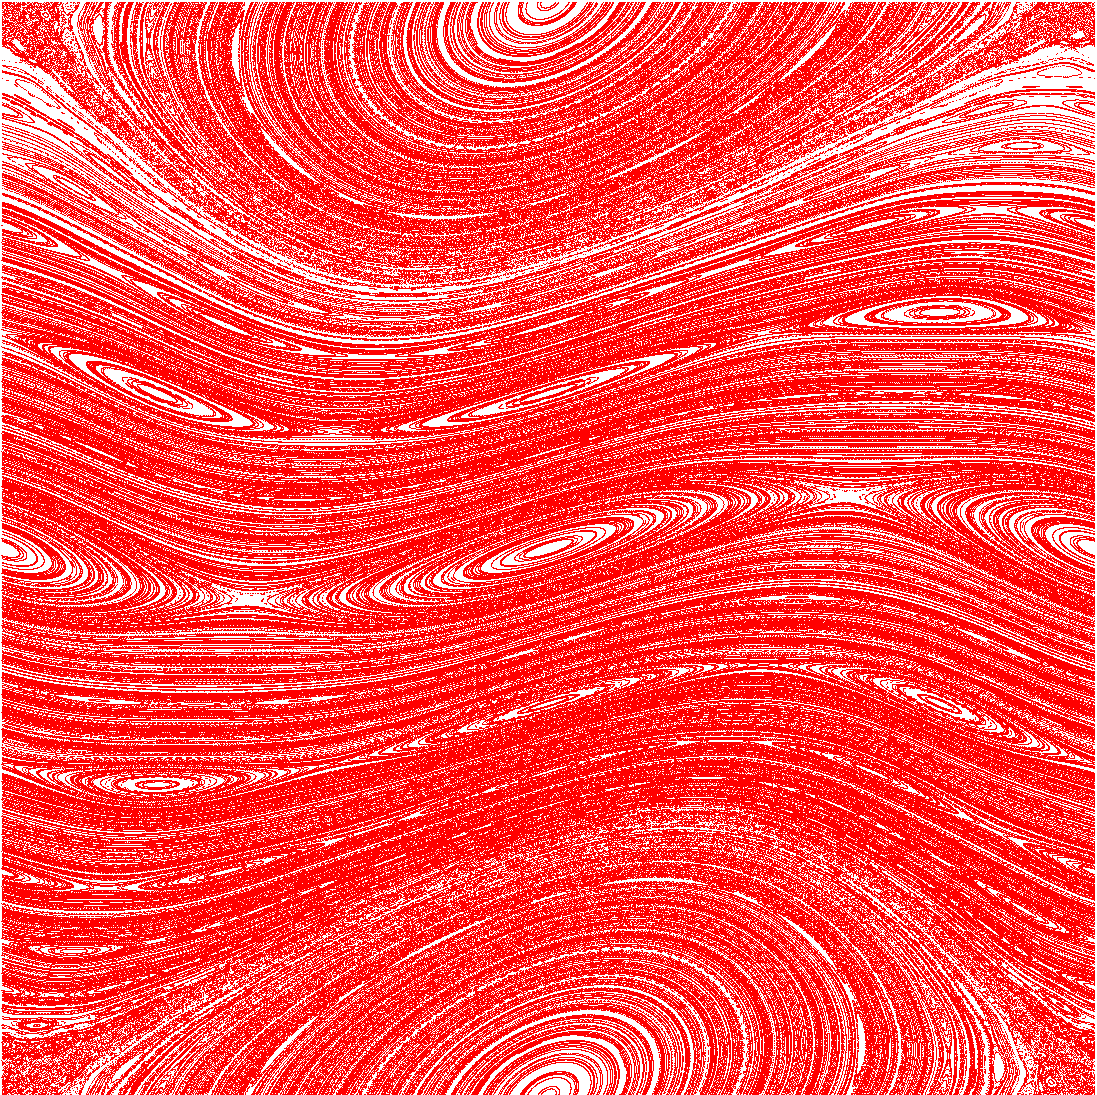
\includegraphics[scale=0.13,trim=0cm 0cm 0cm 0cm]{ch1_litrev/k_0_6.png}
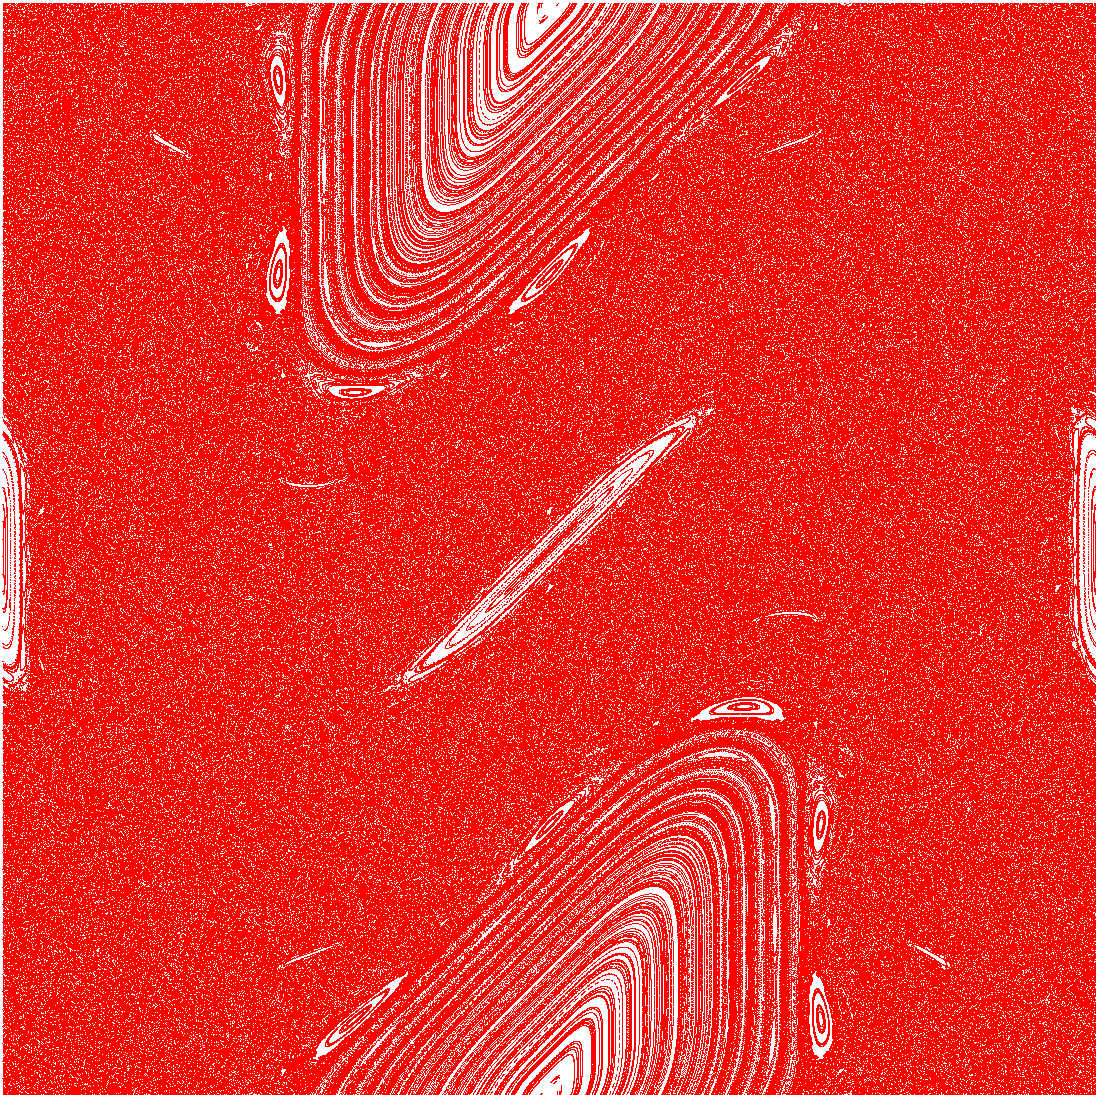
\includegraphics[scale=0.13,trim=0cm 0cm 0cm 0cm]{ch1_litrev/k_2_0.png}

\includegraphics[scale=0.13,trim=0cm 0cm 0cm 0cm]{ch1_litrev/k_12_0.png}
\caption{Images left to right represent phase space states of the classical kicked rotor using the standard map with increasing kicking strength, $K$. The left panel corresponds to $K=0.6$, still showing trajectories; the middle panel is for $K=2.0$, which shows chaos and 3 visible orbit regions; the right panel shows $K=12.0$ yielding a completely chaotic state.}
\label{fig:kickedrotor}
\end{figure}

One widely used model applied to understand such dynamics is that of the kicked rotor \cite{CT:Korsch_ajp_2008}. This model can be thought of as a particle rotating about a fixed point on a ring, receiving periodic kicks, the relative strength and sign of which depend upon the position on the ring. The variables in such a model are the momentum, $p$, which can take any value, and the angle, $\theta$, which is confined to values between 0 and 2$\pi$. The Hamiltonian describing such a system is given by
\begin{equation} \label{eqn:kickedrotor}
H = \frac{p^2}{2m} - K\cos(\theta)\displaystyle\sum_{n=-\infty}^{\infty}\delta(t-n\tau),
\end{equation}
where $K$ represents the kicking strength, and $\delta$ is the Dirac delta function, with $\tau$ being the kicking period. This type of system has been extensively used to understand both classical and quantum chaotic behaviour \cite{CT:Ulah_thesis_2012}. Examples for the trajectories for differing kicking strengths, $K$, are given in Fig. \ref{fig:kickedrotor}. It is easy to see that low kicking strengths give closed orbits, whilst an increase in kicking strength allows the system to enter a globally chaotic regime. The images in the chaotic regime demonstrate the area-filling property of the Poincar\'e section in phase--space.

A related system offering similar behaviour is the delta kicked harmonic oscillator, which modifies the Hamiltonian defined by Eq. \eqref{eqn:kickedrotor}, to include an additional harmonic potential. The resulting Hamiltonian is
\begin{equation}\label{eqn:deltaharmosc}
H = \frac{p^2}{2m} + \frac{m\omega^2 x^2}{2} - K\cos(kx)\displaystyle\sum_{n=-\infty}^{\infty}\delta(t-n\tau),
\end{equation}
where $\omega$ is the frequency of the harmonic potential, and $k=2\pi/\lambda$ is the wavenumber of the periodic potential.  This model can be thought of as a classical particle in a harmonic potential, oscillating and receiving periodic kicks with the strength and sign dependent upon the position within the potential. Gardiner \cite[chap. 4]{THS:Gardiner_2000} discusses this model, and the resulting chaotic behaviour for the classical case and for the quantum case. Variation of the kicking strength and period leads to a variety of interesting dynamics, and the onset of chaos can be observed as the kicking strength increases.

\subsection{Chaos in quantum systems}
The statements characterising chaos given in Section \ref{ss:chaotic} are applicable to classical systems only. One significant difference is that the sensitivity to initial conditions is no longer given due to the unitary nature of the quantum operators \cite{CT:Schack_pre_1996,CT:Gardiner_pra_2000}. The connection between classical chaotic behaviour and quantum mechanics, therefore, remains to be understood as the correspondence principle, given by Bohr, states that quantum dynamics has to reproduce classical dynamics in certain limits. However, classically chaotic systems do not show a quantum counterpart. The hypersensitivity to initial conditions does not appear in quantum systems, and quasiperiodic quantum systems can have a fully chaotic classical equivalent system \cite{CT:Jensen_nat_1992}. As such, the term ``quantum chaos'' has come to refer to
quantum systems which can be described by a Hamiltonian exhibiting chaos in a classical setting. The quantum delta kicked harmonic oscillator, previously described for classical systems, has been studied for its ability to generate chaotic dynamics in works given by Daly \cite{THS:Daly_1994}, Gardiner \cite{THS:Gardiner_2000}, and Kells \textit{et al}. \cite{CT:Kells_pre_2004}. Given the requirement of non-integrability to observe chaotic dynamics, it is worth noting that in the limit where the Schr\"{o}dinger equation is valid the system can be integrable due to its linear nature \cite{THS:Gardiner_2000}. The quantum delta-kicked harmonic oscillator dynamics can be examined by replacing the classical conjugate variables, $(x,p)$, of the Hamiltonian Eq. \eqref{eqn:deltaharmosc}, with their quantum operators, $(\hat{x},\hat{p})$, as
\begin{equation}\label{eqn:hamiltonian_qkick}
\hat{H} = \frac{\hat{p}^2}{2m} + \frac{m\omega^2 \hat{x}^2}{2} - K\cos(k\hat{x})\displaystyle\sum_{n=-\infty}^{\infty}\delta(t-n\tau).
\end{equation}
The dynamics in such a quantum system can be examined using similar tools as the ones presented for classical systems, such as phase-space visualisation. Obtaining a phase-space representation of the wavefunction is, however, not as straightforward as in the classical case. A common method for this involves calculating the Wigner quasiprobability function from the wavefunction.

Experimentally realisable systems that can exhibit such behaviour have recently become accessible, with the delta kicked rotor having been implemented in an optical and condensate system \cite{CT:Ullah_epjd_2012,CT:Lemos_natcomm_2012}. Such systems are, however, still rare. The extension of the above Hamiltonian to non-linear systems described by the Gross--Pitaevskii equation, rather than the linear Schr\"{o}dinger equation, opens up the possibility of observing interesting dynamics. Given that the area of quantum chaos is not as developed as that of classical chaos, the literature is not as well formulated, and tends to be more qualitative than quantitative, barring a few works. The use of Floquet theory is required to fully understand how to analyse periodic quantum chaotic systems, as it is a widely used method applied to describe the quantum behaviour \cite{CT:McCaw_thesis_2005}. Mapping a system onto the Hamiltonian as, for example, the one given by Eq. \eqref{eqn:hamiltonian_qkick}, would provide a way to realise a system that can yield observable chaotic behaviour. For this reason, the proposal given in Section \ref{sec:prelim} will discuss using this Hamiltonian as an integral part of my PhD thesis research.
 % Import your chapters here
        %\section{Thesis proposal}\label{sec:prelim}

\subsection{Project definition}
%I shall begin by restating many of the points covered throughout this literature review: The realisation of condensates was was first given in 1995, following prediction nearly 60 years previously. The behaviour of such systems saw much interest, with theoretical and experimental work seeing a significant rise since this date. One of the properties of condensates, the superfluid nature, received a large degree of attention, with many investigating the nature of quantised vorticity. Approaching the fast rotation limit allows these vortices to enter a crystalline lattice state, analogous to the Abrikosov lattice seen with type-II superconductors subjected to a static magnetic field. This mean-field quantum Hall regime remains predictable using the Gross--Pitaevskii equation, as it is still a weakly correlated state for a range of values beneath the fast-rotation limit. The use of optical lattices with condensates allows for the creation of strongly correlated states, giving a transition between Mott insulator and superfluid regimes by varying lattice intensity. Studies combining vortex lattices and optical lattices have shown transition from Abrikosov to pinned lattice state. Given the fluid superfluid nature of condensates it is possible to study chaos in the quantum regime. The kicked harmonic oscillator lends itself as an ideal model to attempt an understanding of chaos in quantum systems, and has been demonstrated as such.
As part of my PhD I intend to investigate the dynamical behaviour of Bose--Einstein condensates within the fast-rotation limit. With the rotation frequency approaching the trapping frequency of the condensate, the appearance of an Abrikosov (triangular) lattice of vortices in the condensate is expected. This is similar to the type of behaviour observed in type-II superconductors subjected to an applied magnetic field \cite{QM:Abrikosov_jpcs_1957}. With the condensate ground-state having an Abrikosov lattice of vortices, the goal will be to investigate quantum dynamical behaviour in this mean-field quantum Hall regime, with an investigation into chaotic dynamics. This will be carried out by treating the system as a delta-kicked quantum oscillator, where a periodically pulsed optical lattice, whose structure is matched to that of the vortex lattice, is doing the kicking. The plan is to treat the vortex as an effective particle through which the (potentially chaotic) dynamical behaviour may be observed. The Hamiltonian of this system can be mapped to that of the delta-kicked harmonic oscillator Hamiltonian, and will allow for a means to describe the resulting dynamics using an analytical  approach.
%The delta kicking shall be from an intense Gaussian laser field, applied to the vortex position at timescales shorter than the condensate dynamics. However, dealing with a single vortex and single narrow laser is possible, more experimentally realisable, and useful information may be obtained from the use of a large collection of vortices, such as the Abrikosov lattice. The subjecting laser field shall thus be given as that of an optical lattice, with structure matching that of the vortex lattice.

Due to the complex nature of this proposed system, a significant degree of computation will be required. Following on from the methods given in Section \ref{sec:numerics}, one way to perform the large computations required are through use of graphics processing units (GPU). I have previously worked on developing an application for the numerical solution of a fully three-dimensional Schr\"{o}dinger equation in waveguides using GPUs \cite{AO:Morgan_ORiordan_pra_2013}, and I have used this as the basis for the study proposed. I have further modified the developed code to deal with the non-linearity arising from the Gross--Pitaesvkii equation \eqref{eqn:gpe_rotation}, and to account for angular momentum. The resulting code was published under an open-source LGPLv2 license, and named ``GPUE'' \cite{NUM:gpue}. Generalisation of this code will allow more complex quantum systems to be examined, and so far has been shown to achieve results in substantially less time than competing implementations.

%For a thorough understanding of the numerically obtained results, more complex analytics will be considered and applied. For this the Wigner quasi-probability function will be calculated, to allow observation of the phase-space dynamics of the system. I will also apply Floquet theory to this periodic system, which will allow the derivation of analytical results in certain limits. 
%Once the code to determine the ground-state under large rotation is developed, the preparation of a vortex lattice with any specified number of vortices is expected to be numerically possible. Such a system may then be pulsed via briefly applied external potentials. Considering the use of a triangular optical lattice, wherein the lattice spacing is equivalent to the inter-vortex spacing of the condensate, a 1:1 mapping of the optical lattice to the vortex lattice can be achieved within a certain condensate radius. The goal of my project is to create a system in which behaviour akin to that of the delta-kicked quantum oscillator can be observed and to study the potentially chaotic dynamics. Treating the vortex as an effective particle, and the optical lattice potential as a delta perturbation in time, it may be possible to observe signatures of chaos for topological excitations. %Quantification of quantum chaos in experimentally realisable systems, such as superfluid Helium, is a challenging feat \cite{CT:Kobayashi_pra_2007}. The use of dilute condensates instead of superfluid Helium offers much greater ease in observing phase and density, and as such these systems may offer more insight into, and showcasing of the dynamics that can be expected to occur.

To effectively study this system, it will be necessary to obtain a thorough understanding of both classical and quantum chaos for 
Hamiltonian systems. Properties of the system will be analysed, with phase-space methods, such as calculating the Wigner function, which will provide information about the system dynamics \cite{CT:Gardiner_pra_2000}. It will be necessary to calculate the Wigner function for each variation of the condensate system parameters, and further indepth studies using Floquet analysis will be necessary for effective characterization of the observed behaviours \cite{CT:chu_physrep_2004,CT:McCaw_thesis_2005,CT:Gardiner_thesis_2000,CT:Kells_pre_2004}.

\subsection{Overall aims}
For successful completion of this project the following goals are outlined.
\begin{itemize}
	\item Generate a large, stable vortex lattice using a Bose--Einstein condensate within the MFQH regime.\vspace{-1em}
	\item Generate dynamical simulations of BECs using a periodically pulsed optical lattice matched to vortex lattice.\vspace{-1em}
	\item Track the motion of individual vortices in position space, and characterise dynamical behaviour observed.\vspace{-1em}
	\item Analyse the behaviour of the system in phase-space using the Wigner function of the resulting dynamics.\vspace{-1em}
	\item Apply Floquet theory to the system, and infer information about the observed behaviour from the results.
\end{itemize}
Experiments to observe chaotic behaviour in the quantum regime are rare, and the realisation of this type of system should allow for the first of its kind to observe chaos in a system of well-ordered topological excitations. Given recent experimental progress in the area of trapping, cooling, rotating and controlling Bose--Einstein condensates, the proposed system should be realisable with currently available experimental techniques.
The required techniques for theoretically performing this body of work will be described below.

\subsection{Methods and techniques}
\subsubsection{Creating a vortex with phase imprinting}
As a precursor to this proposal, I have performed preliminary work during my time in the Busch unit to investigate the behaviour of condensates with differing numbers of
vortices, and subjected to a short external pulse. Initially, the behaviour of a condensate with a low number of vortices (0,1,2) was examined. 
Numerical integration of the two dimensional Gross--Pitaevskii equation in imaginary time in the co-rotating frame allowed for the
determination of the ground-state in the absence of the perturbation. A predefined winding number, corresponding to the number of vortices required, was applied by multiplication of an appropriate phase with an initial Gaussian guess for the wavefunction guess, and evolved in imaginary time. After that, the resulting numerical ground-state solution was perturbed by kicking it with an additional Gaussian phase pattern, representing a laser pulse (kick), and he system was evolved in real time. A Gaussian phase is
known to give rise to breathing modes in the condensate \cite{BEC:Kimura_pra_2002}, as the velocity of the condensate atoms is given by the 
gradient of its phase. With a kick of large amplitude, the atoms with sufficiently steep phase gradient will move at a greater velocity than those at the
edges or the centre of the Gaussian pulse. As a result, the faster moving atoms will overtake those in the slower moving regions, and due to the
coherent nature of the condensate, matter-wave intereference fringes were observed. From this observation, it is clear that the condensate
under these conditions behaves as an interferometer. With the presence of more than a single Gaussian pulse more complex interference 
patterns can develop and any inhomogeneities in the trapping potential will give rise to a non-symmetric fringe pattern, which may in turn be used to determine the quality of the trap, or the topology of nearby structures. Example results are shown in Fig. \ref{FIG:bec_fringe}.
\begin{figure}[tb]
\begin{center}
	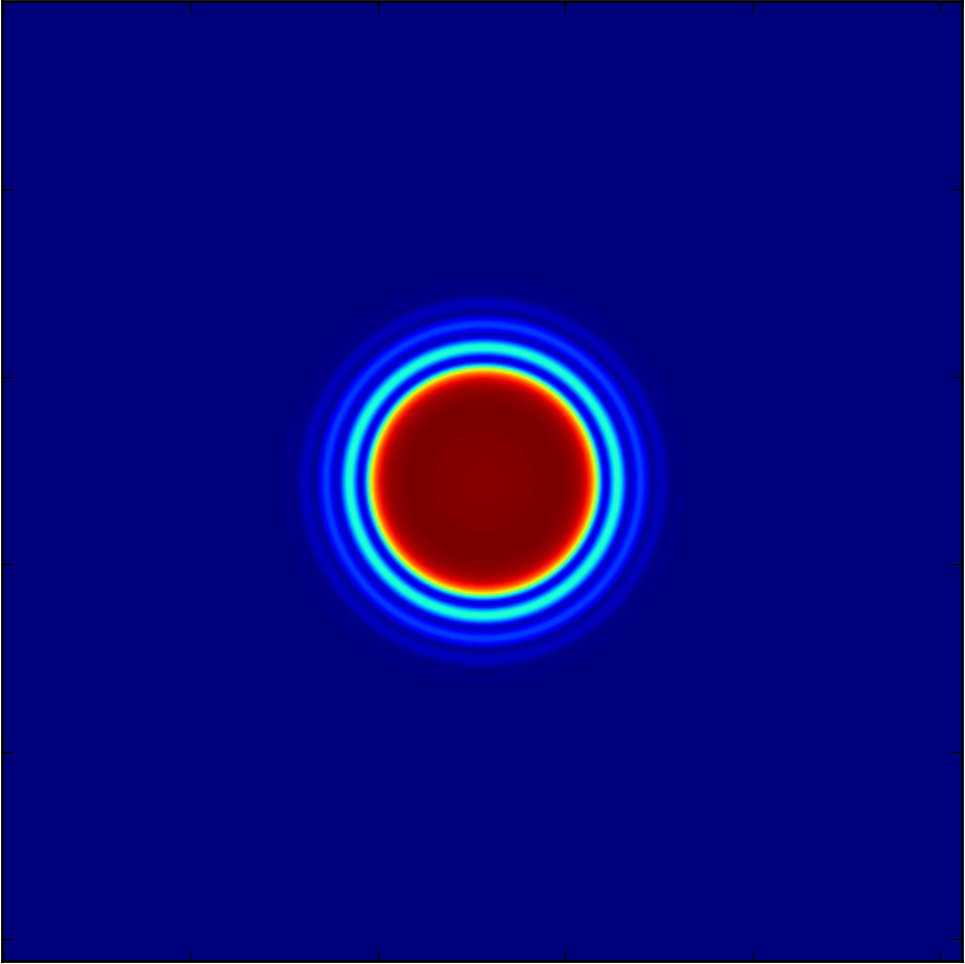
\includegraphics[trim=10cm 10cm 10cm 10cm, clip, scale=0.25,width=3cm]{ch1_litrev/symmetric_guassian_no_vortex_expansion.png}\vspace{0.1em}
	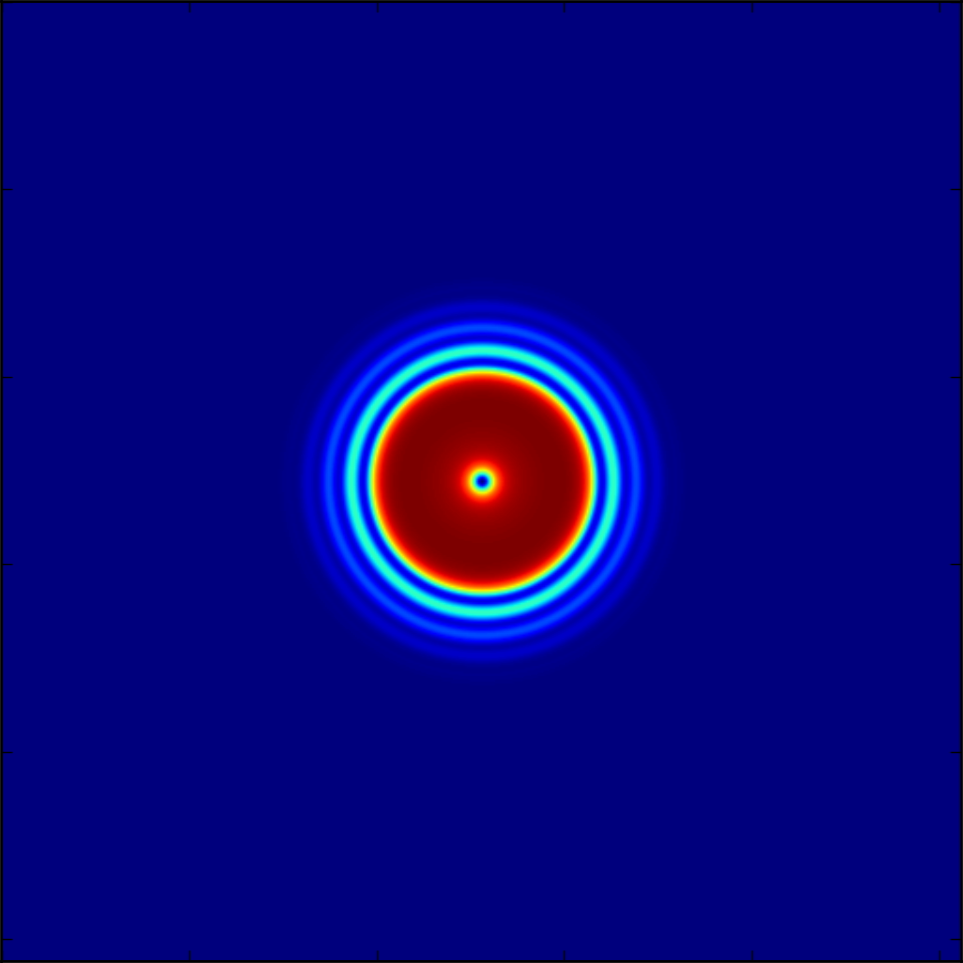
\includegraphics[trim=10cm 10cm 10cm 10cm, clip, scale=0.25,width=3cm]{ch1_litrev/symmetric_gaussian_centre_1vortex_fringe_1stexpansion.png}
	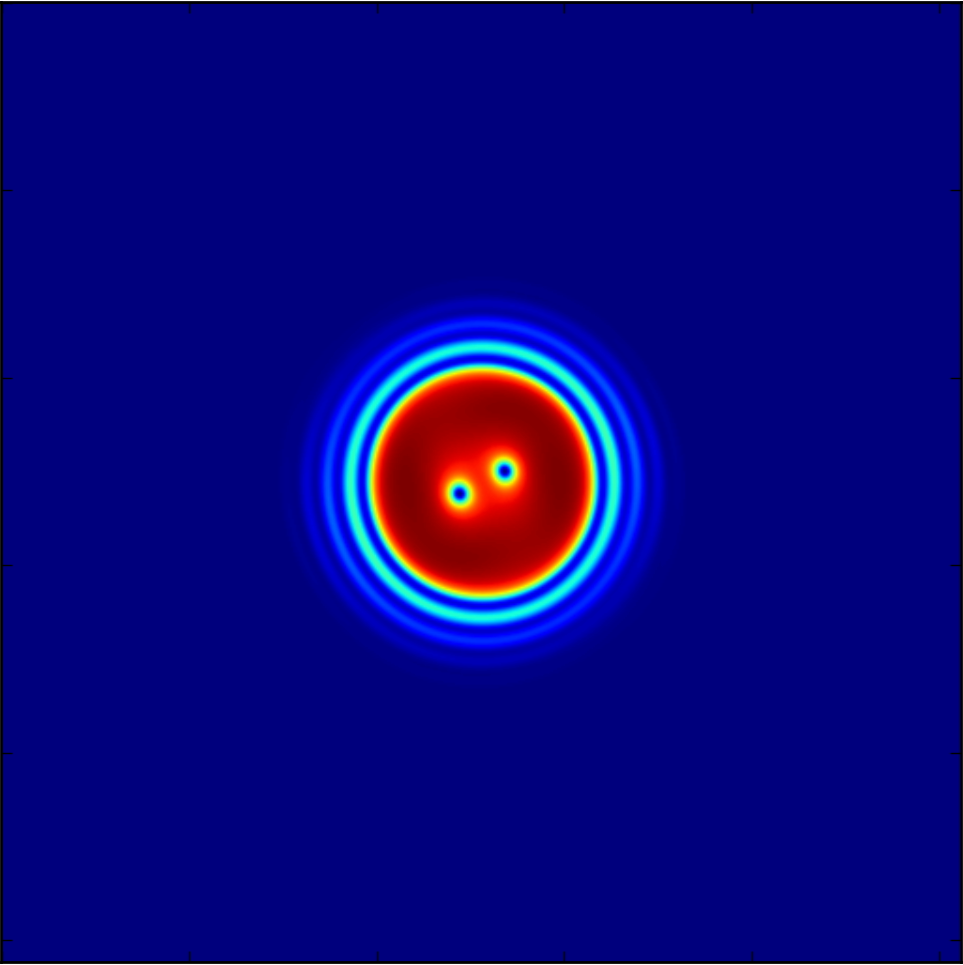
\includegraphics[trim=10cm 10cm 10cm 10cm, clip, scale=0.25,width=3cm]{ch1_litrev/rotating_2vortex_gaussian_centre_1stexpansion.png}
	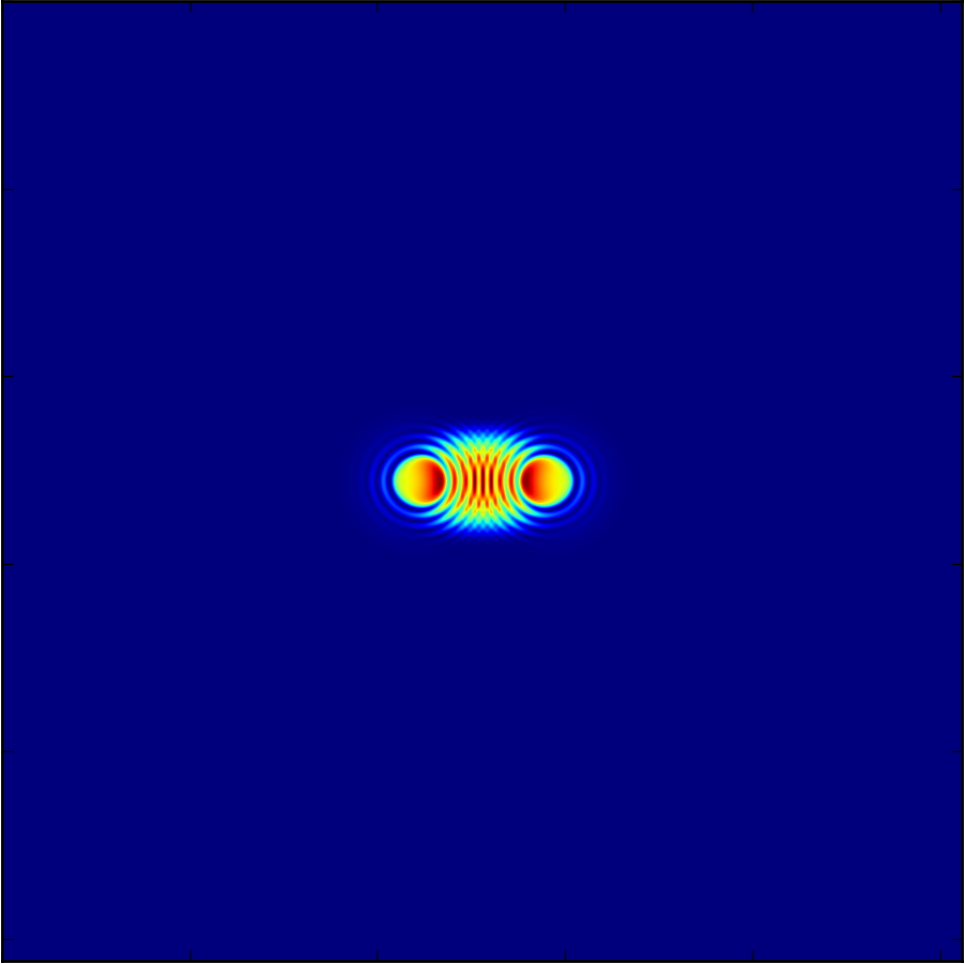
\includegraphics[trim=12cm 12cm 12cm 12cm, clip, scale=0.25,width=3cm,height=3cm]{ch1_litrev/assymetric_0vortex_gaussian_left_right_higher_power.png}
	
	
	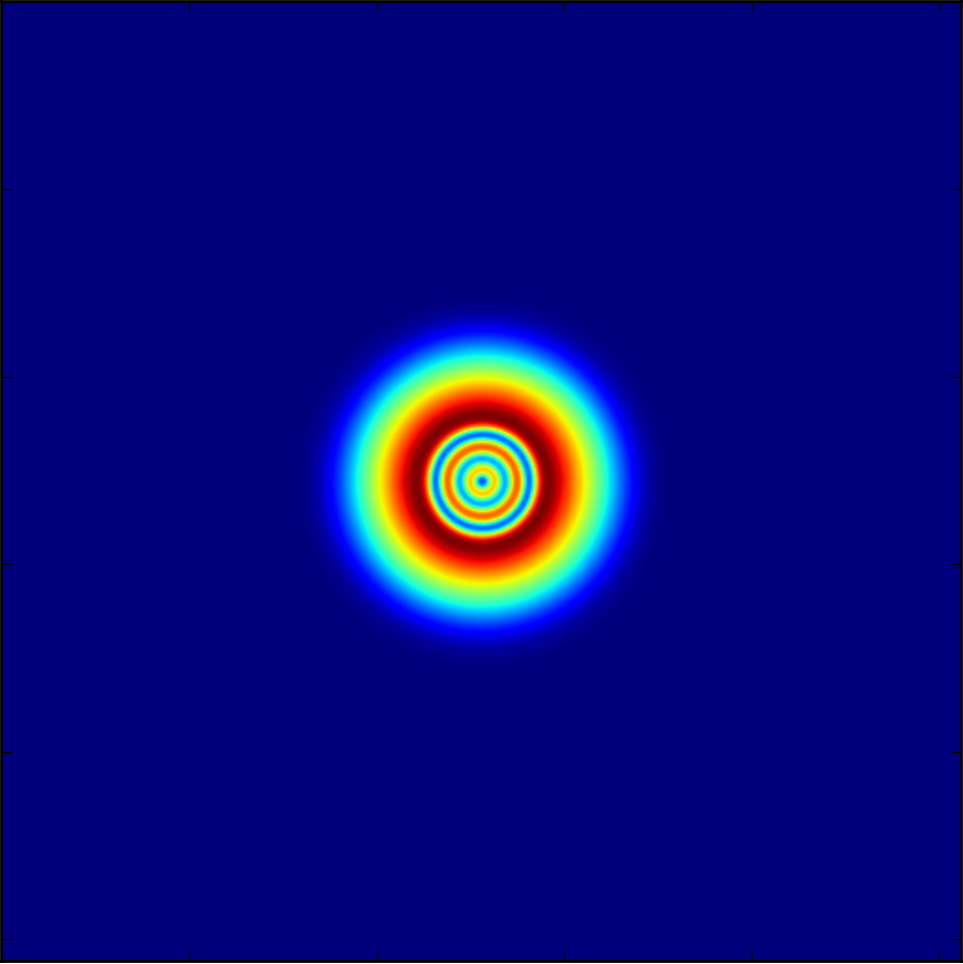
\includegraphics[trim=10.1cm 10cm 10.1cm 10cm, clip, scale=0.25,width=3cm]{ch1_litrev/symmetric_guassian_no_vortex_contraction.png}
	\includegraphics[trim=10.1cm 10cm 10.1cm 10cm, clip, scale=0.25,width=3cm]{ch1_litrev/symmetric_gaussian_centre_1vortex_fringe_1stcontraction.png}
	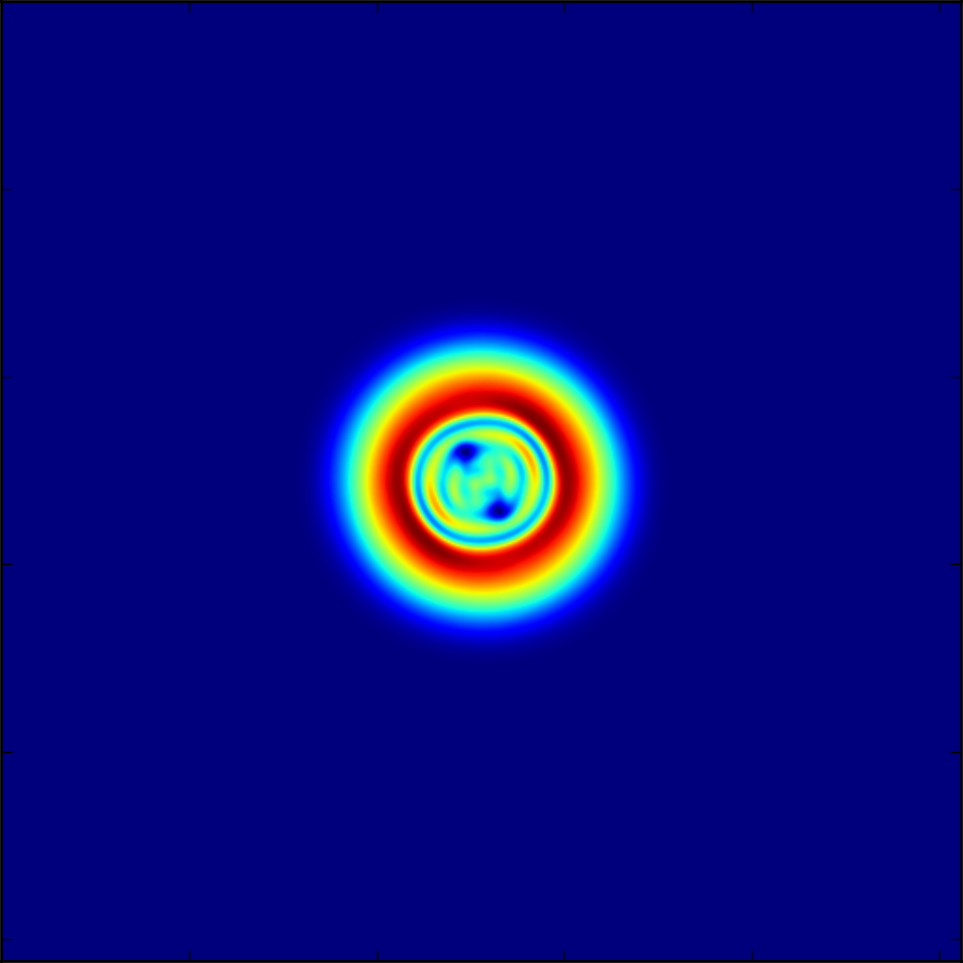
\includegraphics[trim=10.1cm 10cm 10.1cm 10cm, clip, scale=0.25,width=3cm]{ch1_litrev/rotating_2vortex_gaussian_centre_1stcontraction.png}
	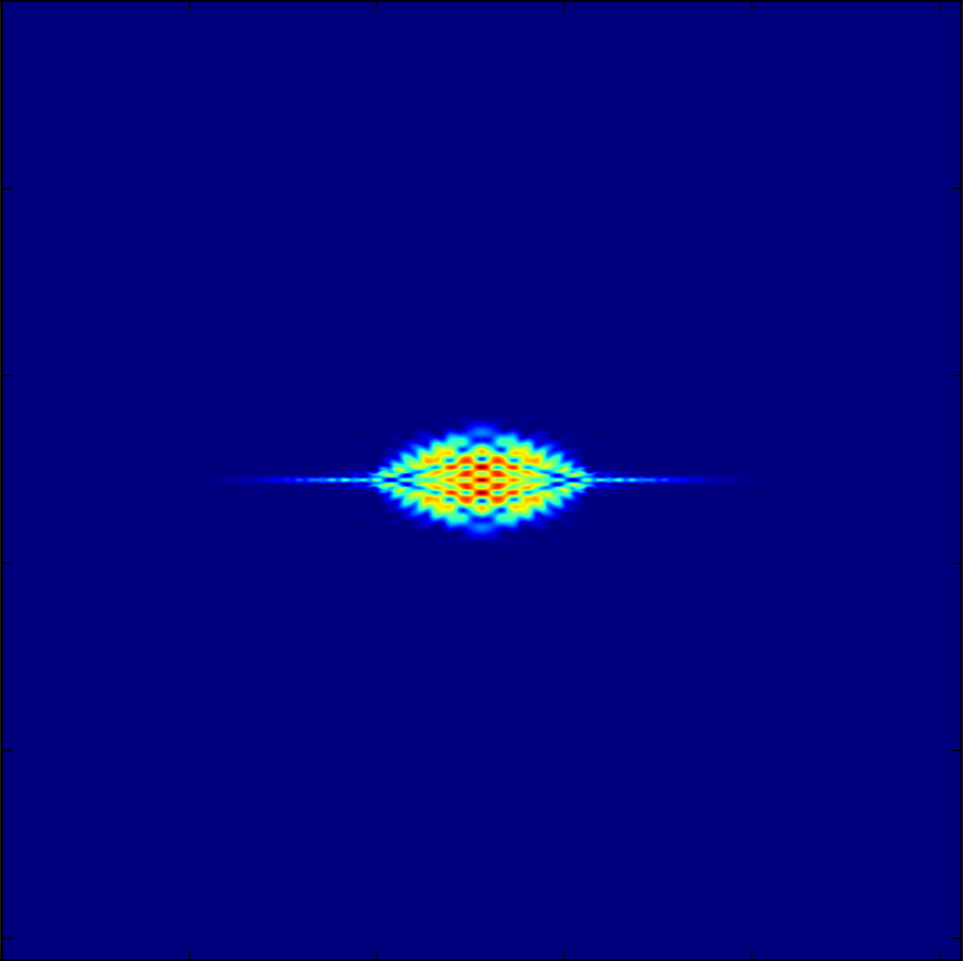
\includegraphics[trim=12cm 12cm 12cm 12cm, clip, scale=0.25,width=3cm,height=3cm]{ch1_litrev/asymetric_novortex_dual_gaussian.png}
	%\includegraphics[trim=10.1cm 10cm 10.1cm 10cm, clip, scale=0.25,width=3cm]{images/symmetric_gaussian_centre_1vortex_fringe_1stcontraction.png}
\end{center}\vspace*{0pt}\caption{Sample results of BECs with varying number of vortices subjected to different phase imprinted patterns. Images are paired top and bottom, at different stages of evolution. From left to right the examined systems are: (i) harmonically trapped condensate with no vortex plus a Gaussian phase in centre; (ii) harmonically trapped condensate with a single vortex plus a Gaussian phase in centre; (iii) harmonically trapped condensate with two vortices plus a Gaussian phase in centre; (iv) anharmonically trapped condensate with no vortex plus two Gaussian phase patterns on opposite sides of condensate\vspace*{-10pt}}\label{FIG:bec_fringe}
\end{figure}

\subsubsection{Creating a vortex lattice}
At low values of the rotation ($0 \leq \Omega \leq 0.49\omega_{\perp}$) the condensate can support a small number of vortices, which when evolved
in imaginary time will form a uniform structure. Increasing the rotation frequency further ($0.5\omega_{\perp} \leq \Omega \leq 0.89\omega_{\perp}$) allows the condensate to support a much larger number of vortices, which can arrange themselves into a lattice pattern. At values approaching the limiting frequency the vortices should order into a large Abrikosov lattice pattern, similar to what
is observed in type-II superconductors. Starting with a large winding number for the phase imprint pattern, the resulting initial guess is evolved in imaginary time, and values approaching the fast rotation limit were chosen. Figure \ref{fig:close_to_abrikosov} shows an example of the condensate under fast rotation, assuming an initial winding of the order 100.
 \begin{figure}[tb]
 \centering
 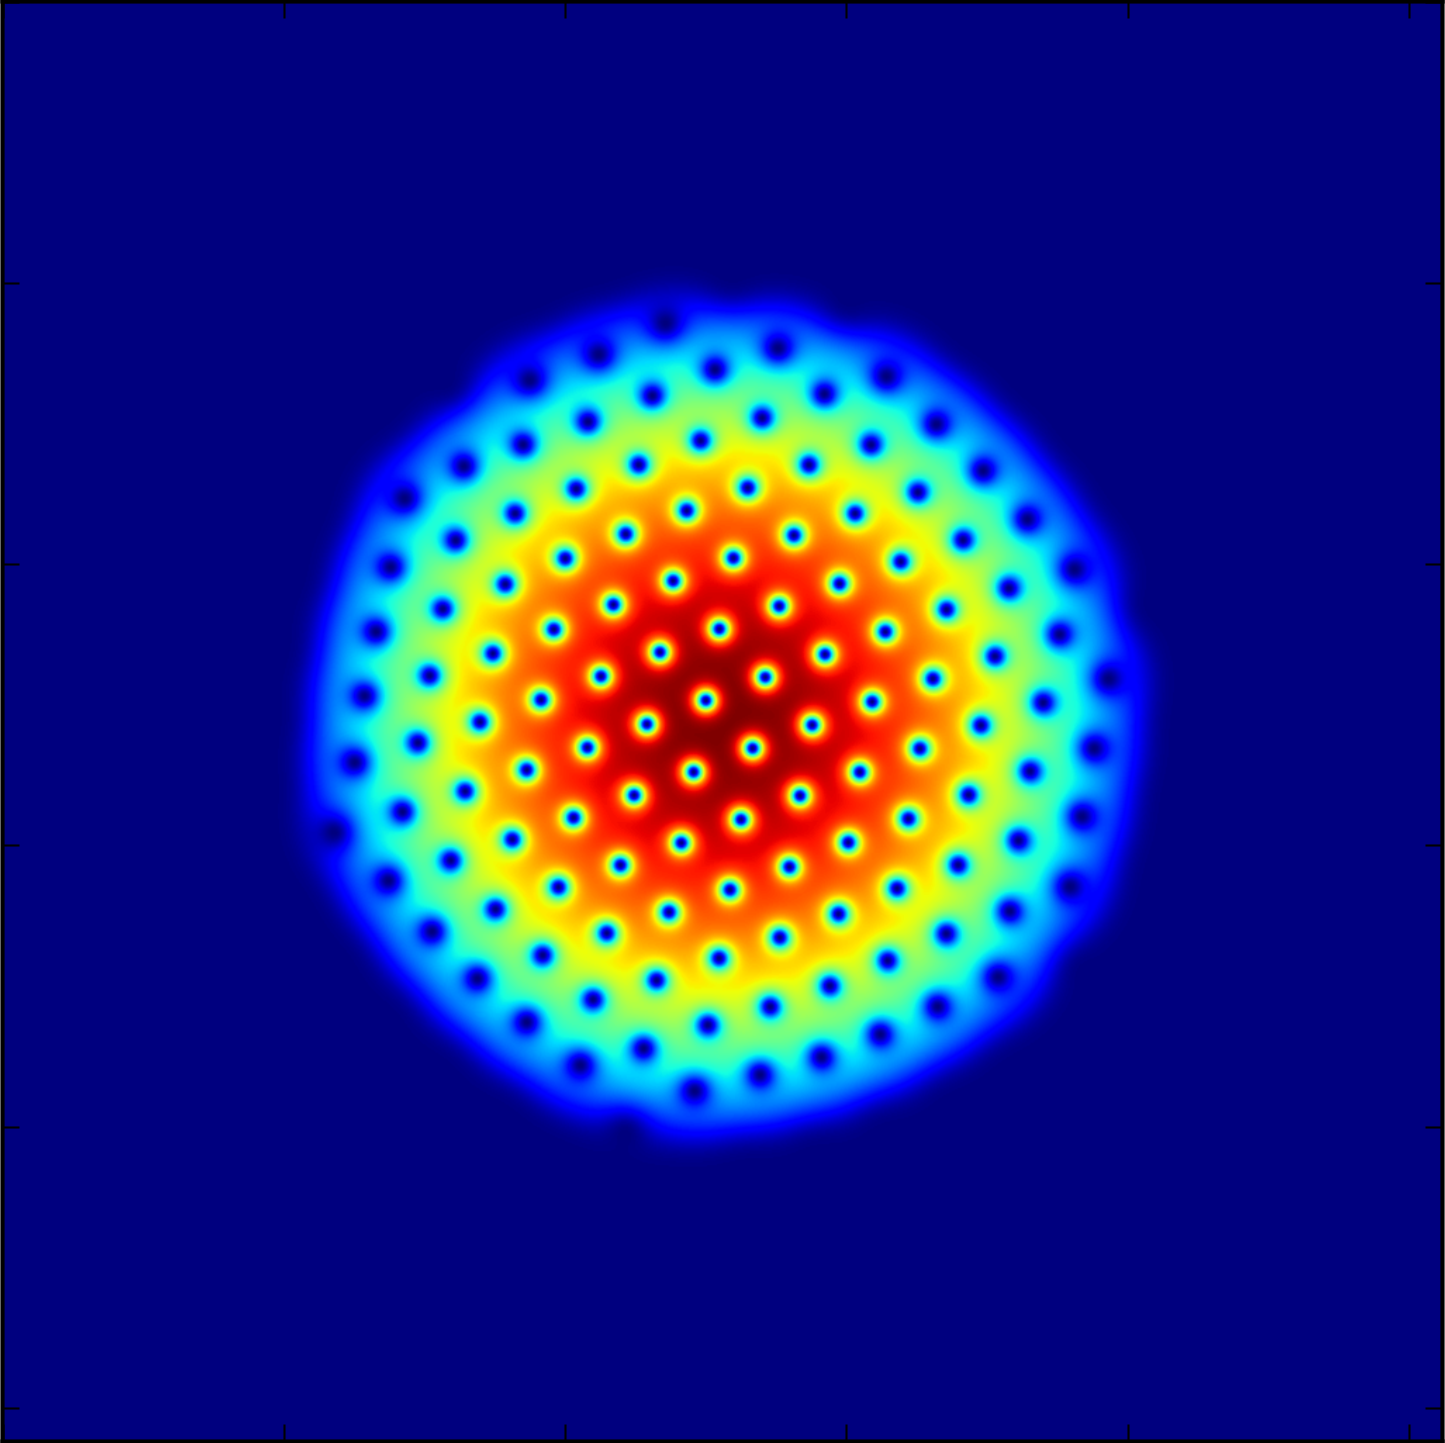
\includegraphics[scale=0.085]{ch1_litrev/wfc_19900000.png}
  \includegraphics[scale=0.085]{ch1_litrev/phi_19900000.png}
  \caption{Images show the ground-state of a condensate rotating at a frequency of $\Omega=0.9\omega_{\perp}$. Even though the Abrikosov lattice is clearly visible, a number of imperfections can be seen in the vortex alignment. Left image shows density, right image shows the phase.}
  %, evaluated at a timestep of $2\times 10^{-6}$ over a grid of $2^{10}\times 2^{10}$
  \label{fig:close_to_abrikosov}
 \end{figure}
To simulate this type of system careful consideration of the angular momentum term in the Hamiltonian must be taken. Initial results have been obtained through use of the GPUE codes that I have developed. However,  the implemented algorithm fails to botain a stable vortex lattice at large rotational frequencies, and so will require an alternative treatment of the system to generate the required state.

\subsubsection{Triangular optical lattice pattern}
For the optical lattice potential, three retroreflected laser fields are considered, giving rise to plane-waves oriented at 0, $\pi/3$ and $2\pi/3$. The resulting fields are defined as 
\begin{equation}\label{eqn:lattice_potential_tri}
V_{opt} = V_0\left[\cos^2\left(k\frac{x-\sqrt{3}y}{2} \right) + \cos^2\left(k\frac{x+\sqrt{3}y}{2} \right) +\cos^2\left(ky\right)\right],
\end{equation}
where $V_0$ is the amplitude of the optical lattice, and $k$ is the wavevector, given by $k=2\pi/\lambda$. A sample resulting optical lattice potential is shown in Fig. \ref{fig:optical_lattice}. The optical wavelength and position can be precisely controlled, even though it is an experimentally challenging task. Given the fine control over condensate parameters, matching the optical lattice to the vortex lattice structure is expected to be experimentally realisable, albeit with cutting edge techniques \cite{Vtx:Tung_prl_2006}.
\begin{figure}
\centering
	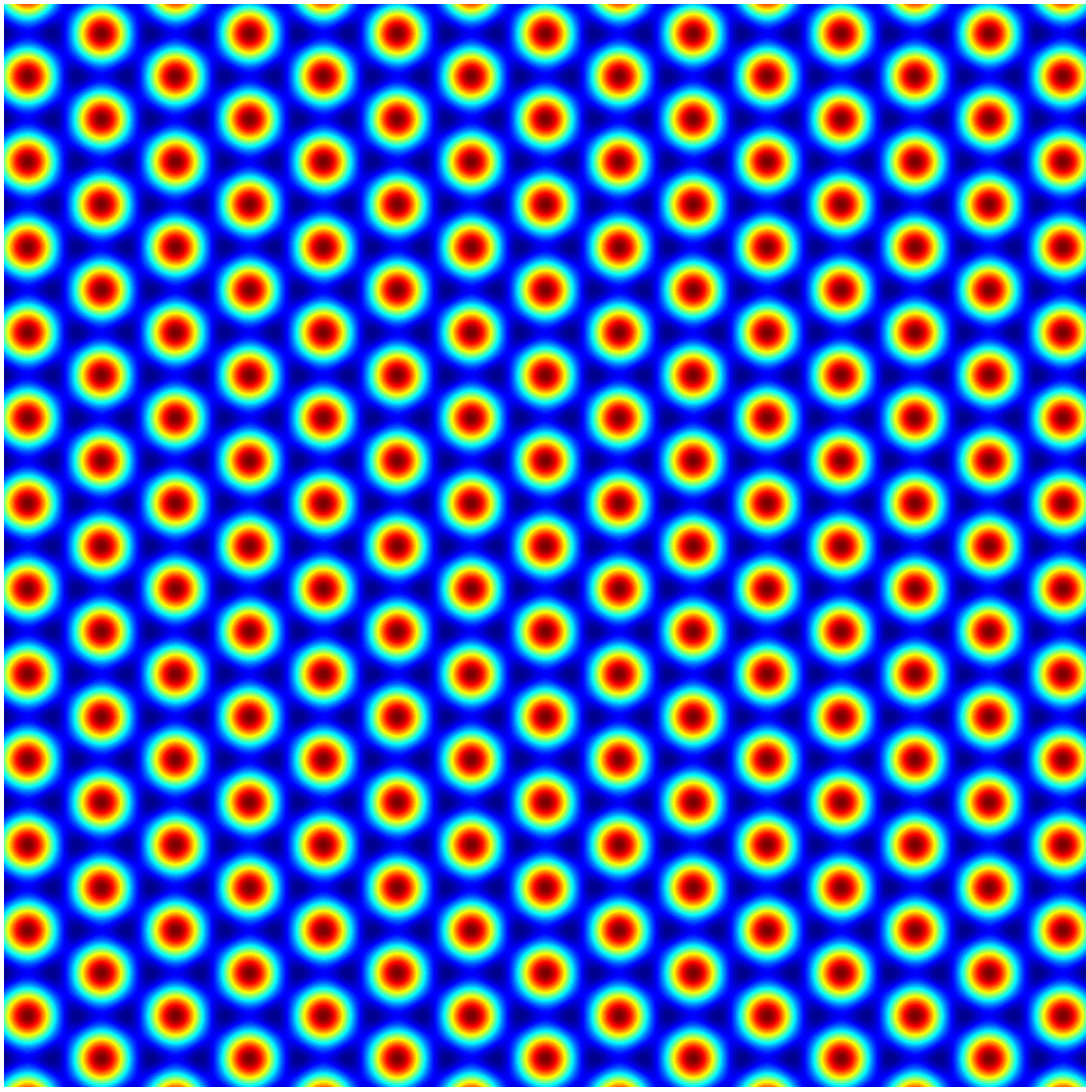
\includegraphics[scale=0.2]{ch1_litrev/opt_latt_g.png}
	\caption{The above image shows a triangular optical lattice potential pattern. This pattern will be adjusted to match the Abrikosov lattice pattern of the condensate in the fast-rotation limit.}\label{fig:optical_lattice}
\end{figure}
To use this optical lattice to generate the expected dynamics in the simulation it will be applied during the real-time evolution. This can be allowed by summing with the trapping potential for an instantaneous pulse of timescale equal to the time-step, or can be applied directly to the condensate phase.

\subsubsection{Delta kicked harmonic oscillator}
Using the Abrikosov lattice pattern with the triangular optical lattice potential we can map this system to the delta-kicked harmonic oscillator, presented in Section \ref{sec:chaos}. In the fast rotation limit, with an Abrikosov lattice pattern of vortices, the lattice undergoes a solid-body rotation. Given that the Abrikosov lattice is a triangular lattice pattern, the system has six-fold rotational symmetry, corresponding with a rotation of $\pi/3$ radians. Thus, a kick applied after a rotation through multiples of this angle will provide a periodic pulsing. The time to rotate through this angle will give the required period, $\tau$, of the system. The amplitude of the optical lattice pattern
will yield the kicking strength, $K$. It is expected that after a yet undetermined number of initial kicks the vortices will start interacting and move from an Abrikosov geometry. After this, all vortices will feel subsequent kicks with a strength dependent upon distance from the maxima and minima of the optical lattice, and should yield some chaotic dynamics. The chaotic dynamics of the system will be investigated by observing the motion of the vortices after a variable total number of kicks, choice of kicking period, lattice size, kicking strength, and a range of interaction strengths for the condensate. Further dynamical behaviour may be determined by calculating the Wigner distribution of the resulting wave-function, and also by analytical analysis using a Floquet theory approach.

\subsection{Significance of proposed work}
The extension between classical and quantum systems remains to be understood. At the classical--quantum limit, the observation of chaos offers a way to gain some insight into processes that may occur. Currently there have been no studies of quantum chaos in systems of topological excitations. Undertaken this project would be the first into investigating such behaviour, and as a result many interesting new physics may be observed. Characterisation of the chaotic behaviour observed in this type of system also will allow for comparative works between the classical and quantum cases. This is a newly developing area of investigation, and the use of condensate use investigating chaotic behaviour has seen few experimental realisations to date. The outlined set-up would allow for a highly controllable system to be subjected to a periodic perturbation relatively easily, mapping it well to the kicked harmonic oscillator. The resulting numerical routines developed should allow for a variety of physical phenomena to be investigated in much shorter timescales compared to currently available methods.

An extension of the work proposed in the project can go in many related directions. One possibility would be to study the transition from the mean-field regime to the strongly correlated (e.g. Mott insulator) regime. The Gross--Pitaevskii theory will no
longer be applicable in this regime, requiring a strict quantum mechanical treatment of bosons. However, it may be possible to formulate some
results for low atom numbers and low vortex numbers in reasonable timescales, again employing GPU computing.  Other possible areas of interest could be the behaviour of such condensates in an open setting, the study of finite temperature effects, differences arising from the dimensionality of the system, the effect of dipolar interactions in the condensate in the fast rotation limit with and without an applied optical potential, multicomponent condensates, and even coherent transport of the condensate in the fast rotation limit.
Another approach to the system discussed above is that of considering interacting charged particles. This can be done by considering each vortex in the lattice as a particle with unit charge, and the application of the delta kicking should lead to the same chaotic behaviour.

\subsection{Caveats}
As mentioned previously, all attempts to generate Abrikosov lattice states have been met with some difficulty. The previously
 used Fourier split-operator method \cite{Num:Bauke_cpc_2011} with Strang-splitting for improved numerical precision \cite{Num:Sanchez_parcomp_2008}, utilised in all previous work appears ill-suited for this system. What has been observed is the inability to effectively find a groundstate of the system
 under fast rotation, approaching the trapping-frequency limit. Some success has been achieved by running a long (several days) simulation (see Fig. \ref{fig:close_to_abrikosov}). However, such long simulation limit the progress which may be achieved. Given the numerical precision required to effectively resolve energies in these systems, new numerical methods must be investigated. One potential way to achieve simulations of condensates in the MFQH regime numerically is through use of the newly defined methods, such as those given by Bao \textit{et al}. and Ming \textit{et al} \cite{Num:Bao_siam_2013,Num:Ming_jcp_2014}. They have reported successful demonstration of numerical codes to investigate rotating condensate behaviour, without the associated difficulties in dealing with the angular momentum operator. It is not yet clear as to whether such methods are applicable to the MFQH regime, as the authors have not demonstrated more than tens of vortices.
 % Import your chapters here
\fi

%%%%%%%%%%%%%%%%%%%%%%%%%%%%%%%%%%%%%%
\newif\ifnumerics
\numericstrue
\ifnumerics
    \chapter{Numerics}
        \section{Numerics}\label{sec:numerics}
For many of the works described previously, it is necessary to apply numerical techniques to obtain results. As the Gross--Pitaevskii
equation, given in Eq. \eqref{eqn:gpe}, is used in the majority of the literature cited, we will consider it as the basis for the following discussion. Given the Gross--Pitaevskii equation, as defined by Eqn. \ref{eqn:gpe}, we can see that it is a second order non-linear partial differential equation. Very few exact solutions exist, and the problem must often be tackled by a numerical approach. Though there are many ways to solve such a system numerically, (such as Crank-Nicholson, Trotter-Suzuki), the method I have chosen is the pseudospectral Fourier split-operator \cite{Num:Bauke_cpc_2011}.

If we consider a unitary evolution operator of the form
\begin{equation}\label{eqn:1}
\Psi(\bar{x},t+\tau) = \exp\left[ -\frac{iH\tau}{\hbar}\right]\Psi(\bar{x},t),
\end{equation}
where $H$ is the Hamiltonian, composed of momentum, potential, non-linear, and rotation terms defined in Eq. \eqref{eqn:gpe}, we can solve for the wavefunction over a specified timescale. However, due to error propagation resulting from numerical integration techniques, it is necessary to employ methods that allow for the highest precision while providing results in useful timescales. To allow for this, careful choice of the numerical integration methods must be taken.  If we take the Hamiltonian, $H$, in terms of its components as a combination of position and momentum space functions we obtain
\begin{equation}\label{eqn:2}
\hat{H} = \hat{H}_{\textbf{r}} + \hat{H}_{\textbf{p}} + \hat{H}_{\textbf{L}},
\end{equation}
where we first neglect the angular momentum operator, $\hat{H}_{\textbf{L}}$, and consider only the two other non-commuting parts $\hat{H}_{\textbf{r}}$, containing the position operator, and $\hat{H}_{\textbf{p}}$, containing the momentum operator. This way we can reduce the error in the numerical integration scheme by using 2nd order Strang-splitting as
\begin{equation}\label{eqn:3}
\exp\left[ -\frac{ i\left(\hat{H}_{\textbf{r}} + \hat{H}_{\textbf{p}}\right)\tau}{\hbar} \right] \approx \exp\left[- \frac{i\hat{H}_{\textbf{r}}\tau}{2\hbar} \right]\exp\left[-\frac{i\hat{H}_{\textbf{p}}\tau}{\hbar}\right]\exp\left[ -\frac{i\hat{H}_{\textbf{r}}\tau}{2\hbar}\right].
\end{equation}
The respective functions can be mapped to the Gross--Pitaevskii equation's position, and momentum terms as
\begin{equation}
\hat{H}_{\textbf{r}} = V(\bar{x}) + g\vert\Psi(\bar{x},t)\vert^2\; \hspace{5em} \hat{H}_{\textbf{p}} = \frac{-\hbar^2}{2m}\nabla^2.
\end{equation}
%\hat{H}_{\textbf{L}} = \Omega L,
Following Bauke \textit{et al}. \cite{Num:Bauke_cpc_2011}, we can numerically solve this differential equation as
\begin{equation}
\Psi\left(\textbf{r},t+\tau\right) = \left[\hat{U}_{\mathbf{r}}\left(t+\frac{\tau}{2}\right) \mathscr{F}^{-1} \left[ \hat{U}_{\mathbf{k}}(t+\tau) \mathscr{F} \left[ \hat{U}_{\mathbf{r}}\left(t+\frac{\tau}{2}\right) \Psi\left(\mathbf{r},t\right) \right] \right] \right]  \\ + O\left(\tau^3\right),
\end{equation}
where $\hat{U}_{r}=e^{-i\hat{H}_{r}(t)\tau/\hbar}$ is the time evolution operator in real space, $\hat{U}_{p}=e^{-i\hat{H}_{p}(t)\tau/\hbar}$ in momentum space,  $\mathscr{F}$ and $\mathscr{F}^{-1}$ are the forward and backwards Fourier transform respectively. Following \cite{BK:Pitaevskii_Stringari_2003} and taking the Madelung transform of the wavefunction given by Eq. \eqref{eqn:madelung}, the phase of the condensate may be given by
\begin{equation}
\theta = \theta_c + \theta_i,
\end{equation}
where $\theta_c$ is the unperturbed condensate phase, and $\theta_i$ is the phase pattern to be imprinted. Thus, upon solving for the initial condensate phase, an additional phase pattern can be imprinted at any time by multiplying the wavefunction by the intended phase pattern. This is in line with the phase imprinting method, as previously introduced by Dobrek \textit{et al}. \cite{Vtx:Dobrek_pra_1999}. The underlying theory of the Fourier split-operator method for the Gross--Pitaevskii equation is given by Javanainen \textit{et al}. \cite{BEC:Javanainen_jphysa_2006}, showing how the choice of non-linearity and operator splitting affects the outcome of the method. The authors arrive at the conclusion that treating the non-linearity and potential terms together with the most current wavefunction definition yields results with an error magnitude that matches those obtained in the Schr\"{o}dinger Fourier split-operator case, indicating its applicability to this type of problem.

\begin{figure}
    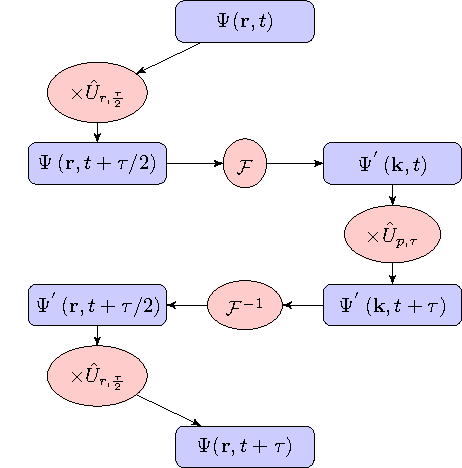
\includegraphics[]{./ch2_numerics/splitop}
    \caption{A single pass through the Fourier split-operator method.}
    \label{fig:num_splitop}
\end{figure}

\section{Angular momentum operators using FSO method}
The Fourier split-operator method described earlier works well in handing cases where the operators live in position or momentum space respectively. However, the angular momentum operators are essentially a combination of both spaces as we deal with each basis respectively. Take, for example, the angular momentum operator along the $z$-axis, given by $L_z = xp_y - yp_x$. To apply $L_z$ we must take not that the $x$ and $y$ components of the wavefunction must be in alternating bases for the evolution. Thus, to apply this operator we must Fourier transform along a single dimension, multiply by the respective operator, take the inverse, and perform this operation along the other dimension.

 This, however, accrues an error not encountered using non-pseudospectral methods. The error can be determined by checking the commutativity of the respective components of the angular momentum operator as
 \begin{align}
 	L_1 = [x p_y,-y p_x] &= [x p_y,-y] p_x  -  y[x p_y,p_x], \\
 				   &= -[-y,x p_y] p_x + y [p_x, x p_y], \\
 				   &= -\left( {\cancelto{0}{[-y,x]}} p_y + x [-y,p_y] \right) p_x + y \left( [p_x,x] p_y + x {\cancelto{0}{[p_x,p_y]}} \right), \\
 				   &= -x {\cancelto{i\hbar}{[-y, p_y]}} p_x + y {\cancelto{-i\hbar}{[p_x,x]}} p_y, \\
 				   &= -i\hbar \left(x p_x + y p_y \right).
 \end{align}

 The complex error term can be seen as, in the case of the implemented evolution, allowing the angular momentum opeartor to change from imaginary time to real-time, and vice-versa in each respective case. To overcome this, we simply swap the application order of the operator components, between even and odd steps during the evolution. Starting with the alternate order we obtain a value of $L_2 = [-y p_x, x p_y] = i\hbar \left(x p_x + y p_y \right)$. Since we are applying this phase to the condensate we can overcome the error of one term by the application of the other, as
 \begin{equation}
 \exp{i L_1}\exp{i L_2} = 1.
 \end{equation}

 Although alternating will provide a cancellation of this error, it can be assumed that for large timesteps the error will have a non-insignificant contribution to the overall dynamics. Thus, for this method to remain accurate we can perform the previous decomposition for a third-order accurate scheme, or use as is for a second-order accurate scheme.

 \subsection{Time evolution}
 To create the initial state for the desired evolution the ground-state of the Hamiltonian needs to be determined as a first step. This can be achieved by evolving the system in imaginary time, where $t\rightarrow it$. This causes all higher energy terms in an initial guess for the condensate wavefunction to decay to zero, leaving the lowest energy state, which corresponds to the ground-state. As effective as this approach may be, the convergence to the lowest lying energy state becomes less effective as the computation approaches the expected value \cite{Vtx:Danaila_pra_2005}. Although many such methods exist, the one that is best suited for this task is that of a Fourier split-operator method. Due to the way the algorithm operates, it is essential to have a large and finely sampled grid in order to resolve both position and momentum of the wavefunction. A minimum grid-size on the order of $2^8$ in 2D for both $X$ and $Y$ dimensions is required. An implementation of such a method at the defined resolution is a straight-forward process using MATLAB, and has been performed for the purpose of this study. However, due to the large computational overhead required to deal with such a calculation, the procedure takes a long time to evolve the system to the necessary degree of accuracy. Therefore, it is necessary to further develop the methods used, and to improve the implementation of this algorithm to leverage the recent advances in computational acceleration.








We can write the wavefunction of a quantum system as a linear superposition of states as
\begin{equation}
     |\Psi \rangle = \displaystyle\sum\limits_{n} C_n |\Psi_n \rangle,
\end{equation}
where $| \Psi_n \rangle$ are a set of basis states for the system, with complex coefficients $C_n$. We next assume a unitary evolution operator of the form
\begin{equation}
    \mathscr{U}(t,t_0) = \exp\left(\frac{-i\mathcal{H}(t-t_0)}{\hbar}\right),
\end{equation}
where $\mathcal{H}$ is the Hamiltonian of the system. To time evolve our system from some time $t_0$ to a final time $t$ we apply the evolution operator to the wavefunction, giving
\begin{equation}
    \mathscr{U}(t,t_0)|\Psi \rangle = \displaystyle\sum\limits_{n} C_n \exp\left(\frac{-i{E_n}(t-t_0)}{\hbar}\right)|\Psi_n \rangle,
\end{equation}
where I have replaced the Hamiltonian operator with the energy eigenvalue of the $n$-th state. It follows from here that each state evolves at a different rate, proportional to its given eigenenergy. Higher energy states will oscillate faster than those of lower energy states. However, to make accurate predictions it is often necessary to deal with a single quantum state, such as the lowest lying state. We can learn much from a quantum system's lowest energy state, and so to evaluate this would be very useful. Taking the evolution operator, we apply a Wick rotation, rotating the time component through $\pi/2$ into the imaginary plane, as $t \rightarrow -it$. Applying this new evolution operator to the wavefunction gives
\begin{equation}
        \mathscr{U^{'}}(t,t_0)|\Psi \rangle = \displaystyle\sum\limits_{n} C_n \exp\left(\frac{-{E_n}(t-t_0)}{\hbar}\right)|\Psi_n \rangle.
\end{equation}
The we have removed the complex term in the operator, which now takes the form of an exponentially decaying operator. When applied to the wavefunction all higher energy terms will decay at a rate faster than lower energy components. This process also causes a loss of probability density, and so the wavefunction must be renormalised after application. Through repeated application of this operator, and a renormalisation afterwards, the quantum system can converge to the groundstate. To begin, however, we must assume an intial guess for the wavefunction, which has some finite overlap with the lowest lying state.











 \section{Vortex tracking}
 To efficiently follow the vortex dynamics, some robust algorithm is needed to track their positions. We could track regions where the density drops to zero. However, this gives very little information on the topological excitation, and may mistake density dips for the presence of such excitations. Thus, one of the most effective ways is to locate the $\pm 2\pi$ charge in the wavefunction phase, which is a signature of quantum vortices. For this, we can assume that around a $2\times 2$ subgrid, the phase rotates from $-\pi$ to $+\pi$ in the presence of a vortex located on the subgrid. After an initial pass to determine the vortex locations closest the nearest grid element, a least-squares fit is performed to more accurately determine the vortex core position. With this, we can accurately the determine the motion of the vortices with high precision.

 To track the vortices during the evolution, the creation of an initial list of vortices is performed, with each given a unique identifier. Assuming the vortex cores can travel a limited distance (some multiple of the grid resolution) between time steps, we can say at subsequent times which vortex has moved to the newly found positions. This is performed through use of a linked list of vortices, each with an assigned unique identifier, associated location, phase winding and on/off flag. A finite boundary is chosen to examine only vortices at the center, which can cause vortices to appear and disappear on the boundary. Thus, any vortex which appears without association to an initial vortex, or any vortex that leaves the boundary, is switched off and remains so for all analysis.

        \section{General purpose GPU computing}

As mentioned earlier, with the increase in dimensionality of a problem, so often too does the time required for performing simulations. It can become necessary to find ways of optimising the use of computational resources to reach a result in a much shorter amount of time. One such method for accelerating numerical solutions involves the use of multiple compute cores on a central processing unit (CPU) operating independently on different data elements in unison. This form of parallel computation can be achieved through the use of the OpenMP (Open Multi-Processing) application programming interface (API), which defines how a program may parallelise certain elements of code. It allows the developer to fully utilise the power of a multicore processor. However, the limit on how much performance can be gained by this method is set by the number of compute cores available to the system, as well as the limited support offered by compilers. It should also be noted that MATLAB has inherent support for such programming paradigms, and fully abstracts the implementation from the developer. Therefore, in this instance writing a program from scratch in C/C++/Python/etc. for such a means of parallelisation would not be very beneficial due to the cost of diminsishing returns. Results would likely be obtained much faster from simply using an already multicore supported package, provided one includes the time to write, as well as simulate. However, this is not always the case, given the size of problems can often require more than the cores available on a single machine.

Another widely used programming paradigm that gets around this is that of MPI (message passing interface). Where OpenMP allows a user to utilise all available processors on a single system, MPI allows the use of an (almost) unlimited number of computer systems operating in parallel together, each known as a node. This is the method generally preferred in programs written for compute clusters, where a large number of nodes are available to use. It is the preferable choice for distributed computing applications, with the best performance gains given if there is minimal dependence between data. A bottleneck may occur if data spread over multiple nodes is required for an operation, requiring continual transmission of data between individual nodes. At current data rates this would be limited to bus speeds of (assuming an Infiniband optical connections) on the order of ten gigabytes per second. Compared to a local calculation requiring little to no transfers, the memory bandwidth (time between the CPU and local memory) can be as high as 60 gigabytes per second \cite{DAT:Intel_xeon}, or greater. Therefore, it is important to note that transfers should be minimised to avoid bottlenecks, but transfers are often necessary to make use of the large number of processing cores. Therefore, to give a significant performance benefit, a large number of cores, a high memory bandwidth, a high-speed interconnect between cores (nodes), as well as sufficient space to store the problem in memory are required. This is a tall order.

One possible means of achieving this high performance is through the use of graphics processing units (GPUs). GPUs are signal processing devices, and have been highly developed over the past 20 years to offload much of the computation required to display images from the central processing unit (CPU). As a result, GPUs have been given the task of performing operations necessary to update a large number of pixels in a short amount of time, as well complex 3D math for image rendering. This has been achieved through giving the GPUs a large number of specialised compute cores for floating-point arithmetic, effectively operating in parallel. With the advent of general purpose GPU (GPGPU) computing, the ability to exploit these cores for the purpose of numerical computing has become possible. A problem can be mapped to the hardware of a GPU, and all parallelisable operations can be accelerated, reducing the overall compute overhead required for evaluating results. For the latest generation of industry standard GPUs used in computational acceleration the memory bandwidth for the device global memory (equivalent of RAM) is given as 288 gigabytes per second, with almost 3000 cores on demand, yielding a theoretical total of $1.41\times10^{12}$, floating-point operations per second (FLOPS), following the formula
\begin{equation}
    \text{FLOPS} = \text{cores}\times\text{clock freq.}\times\text{ops. per clock cycle}.
\end{equation}

In comparison to this are Intel Xeon CPU throughput values, which yield approximately $1\times10^{11}$ FLOPS. As can be seen, performance of an order of magnitude can be gained by using a GPU for calculations, over high-performance (Xeon) CPUs. This has been shown to allow for effective implementation of the previously mentioned Fourier split-operator method \cite{Num:Bauke_cpc_2011}. We have also shown that it yields performance exceeding that of CPU's for a modest choice of GPU \cite{AO:Morgan_ORiordan_pra_2013}, of which I will discuss in detail in a later section.

\subsection{Parallel operations}
\label{sub:Parallel operations}
For a calculation to fully utilise all available throughput of a parallel-capable
compute device, it is essential to break down the problem into easily parallelised (emabarrassingly parallel) sub-problems. Considering summation as an example, imagine we have a large vector of floating point values that are to be summed together. The traditional way to solve this would be to iteratively add values to an accumulator, and return the final value at the end as the sum. This simple algorithm is $\mathcal{O}(n)$ complexity, as we iterate through each element at a time. Given that summation is associative, we easily parallelise this operation. By dividing our vector amongst a number of available processing cores recursively, we can reduce the computation to $\mathcal{O}(\log{} n)$. This algorithm can give a significant benefit when a large number of summations are performed.

\begin{figure}
    \centering
    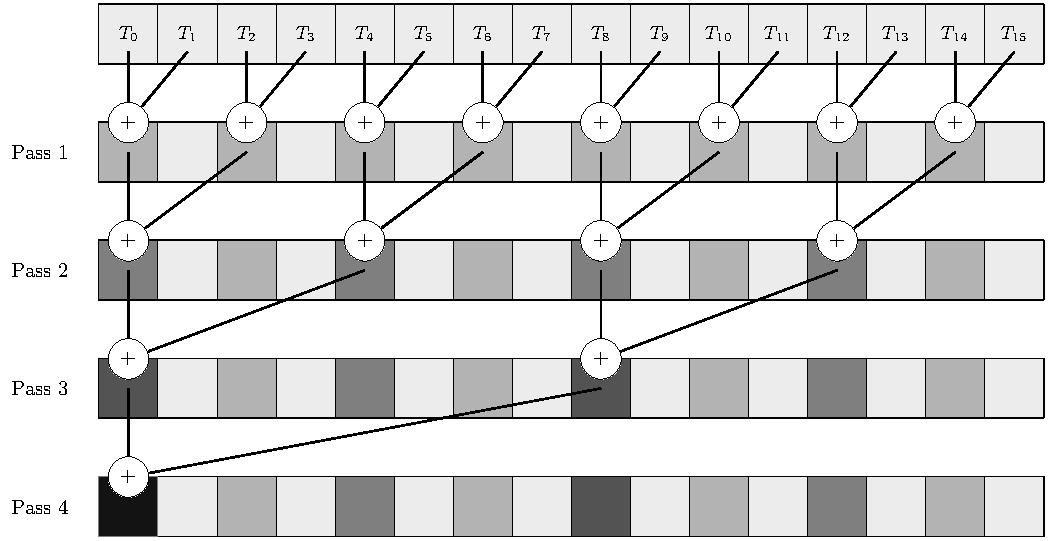
\includegraphics[width=0.75\textwidth]{./ch2_numerics/CUDA/prefixsum.pdf}
    \caption{Parallel summation algorithm. After each pass the number of elements to sum is halved, leading to a $\mathcal{O}(\log{} n)$ complexity in time. Since we require only the total sum, this algorithm choses to read the value at $T_0$ at the end of the run.}
    \label{fig:prefixsum}
\end{figure}

Another typical algorithm following this logic is the Hadamard product (element-wise multiplication) of two vectors, or matices. Although in parallel the number of operations and complexity remains the same, the advantage comes from the lack of interdependence between elements. The multiplications can be carried out asynchronously, allowing all freely available cores to work continuously until every element pair is multiplied.

\begin{figure}
    \centering
    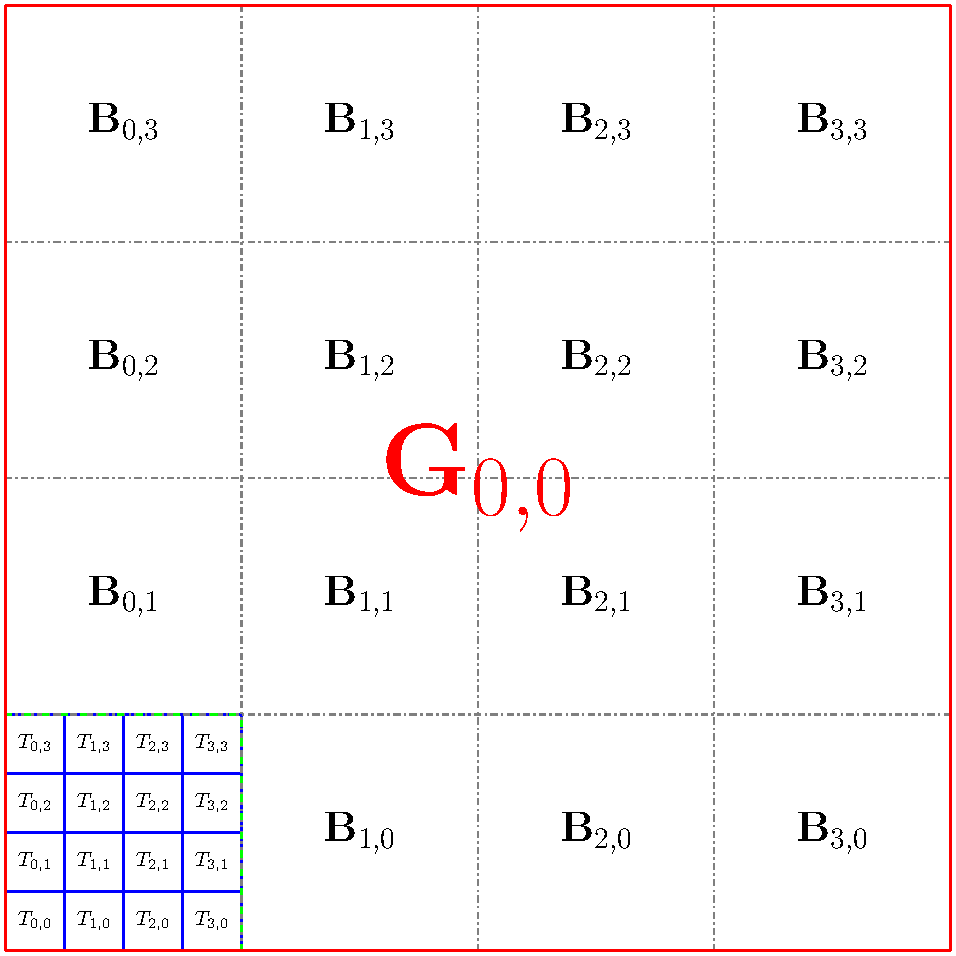
\includegraphics[width=0.75\textwidth]{./ch2_numerics/CUDA/gputhreads.pdf}
    \caption{GPU threads, blocks, grid breakdown.}
    \label{fig:gpu_threads}
\end{figure}

Given that GPUs are first and foremost image processing devices, their ability to perform Fourier transforms rapidly should be a well developed strength. It is. Given the large number of available cores, FFTs can be significantly faster on a GPU than performing the same operation on many CPUs \cite{AO:Morgan_ORiordan_pra_2013}. The CUFFT (Cuda FFT) library allows for a seamless way to take advantage of this performance increase using GPUs, with performance gains discussed in the following section.

\section{3D STIRAP using GPU}
For performance metrics, I will discuss the use of a GPU-enabled Schrodinger equation integrator developed by myself, comparing the results to a multi-core MPI enabled version by T. Morgan and N. Crowley. We solved the Schrodinger equation for a fully three-dimensional potential, demonstrating its accuracy and improved performance compared to standard HPC methods.

        \section{GPUE: GPU Gross--Pitaevskii equation solver}

As mentioned previously, the split operator method makes use of Fourier transforms as a way to change between position space and momentum space. To speed this up, the GPU accelerated CUFFT library is used, allowing for a much faster FFT than can be performed on a single (or across multiple) traditional CPU nodes. However, to take advantage of the GPUs performance, it is essential to minimise the data transfer between host machine (CPU) and device (GPU). Therefore, the remaining operations for the evolution must also be carried out on the GPU. This also requires that the workload is evenly distributed across the cores on the GPU so that we minimise the number of threads that are not performing computations.

Given that the problem of simulating the GPE in a rapidly rotating regime can be modeled as two-dimensional, we can put a limit on the


\begin{figure}
    \centering
    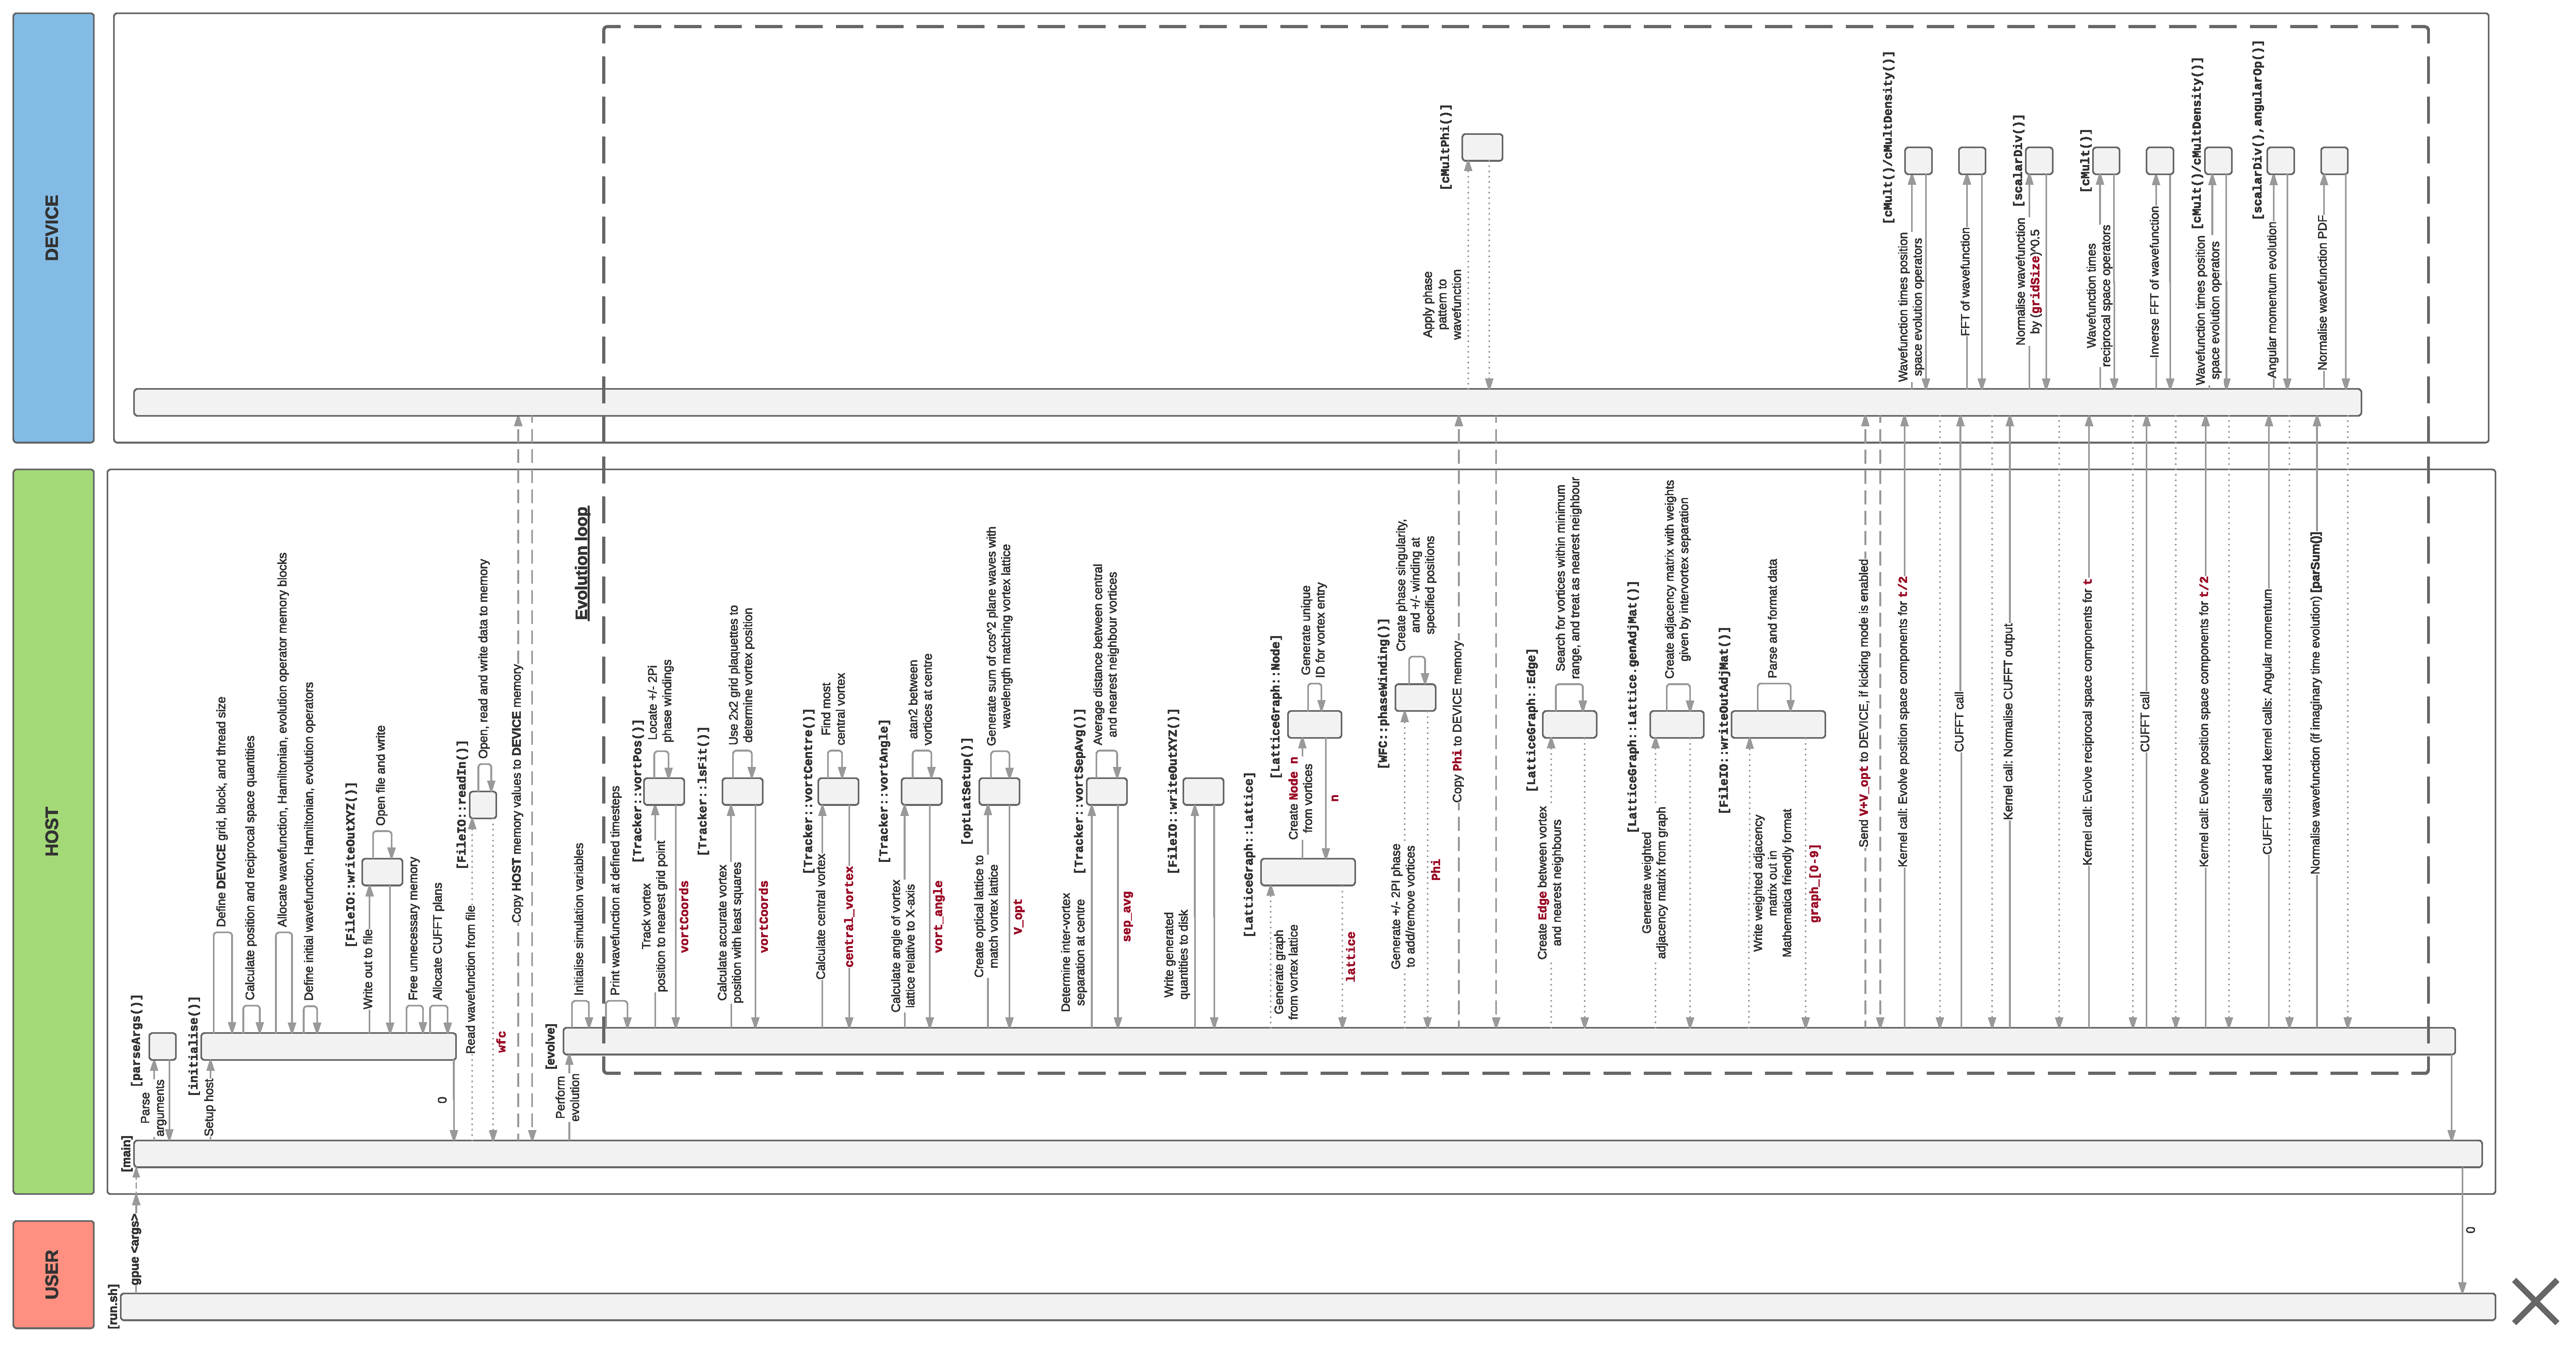
\includegraphics[width=1.5\textwidth,angle=270]{ch2_numerics/GPUE_Seq}
    \caption{Simplified combined sequence and state diagram for GPUE operation.}
    \label{fig:gpue_seq}
\end{figure}

        \section{Bogoliubov equations}
\label{sec:bogo}


Bogo tbc
\begin{equation}\label{eqn:bogo_psi}
\Psi_0(\mathbf{r},t) = \exp\left(-i\frac{\mu t}{\hbar}\right)[\phi_0(\mathbf{r}) + u(\mathbf{r})\exp\left(-i\omega t\right) + v^{*}(\mathbf{r})\exp\left(i\omega t\right) ]
\end{equation}



\begin{equation}\label{eqn:bogo_h0}
H_0 = -\frac{\hbar^2}{2m}\nabla^2 + V(\mathbf{r}) + 2g\vert \phi_0 \vert^2
\end{equation}

\begin{equation}\label{eqn:bogo_lhs}
    \partial_t \Psi(\mathbf{r},t) = \exp\left(\frac{-i\mu t}{\hbar}\right)\left[\mu\phi_0 + (\mu+\hbar\omega)u\exp\left(-it\omega\right) + (\mu+\hbar\omega)v^{*}\exp\left(it\omega\right) \right]
\end{equation}

\begin{align}\label{eqn:bogo_nonlin}
    g|\Psi|^2\Psi &= g \phi_0^{*}\phi_0\phi_0 \\
                &= g\exp\left(\frac{-i\mu t}{\hbar}\right)\left(\phi_0^{*} + u^{*}\exp(i\omega t) + v\exp(-i\omega t)\right)\left(\phi_0 + u\exp(-i\omega t) + v^{*}\exp(i\omega t)\right)^2 \\
                & \approx g\exp\left(\frac{-i\mu t}{\hbar}\right)\left[
                |\phi_0|^2\left(
                 \phi_0 + 2(u\exp\left(-i\omega t\right) + v^{*}\exp\left(i\omega t\right) )\right) + \phi_0^2\left( u^{*}\exp\left(i\omega t\right) + v\exp\left(-i\omega t\right)
                \right)
                \right]
\end{align}
Equating terms gives
\begin{subequations}\label{eqn:bogo_lhsrhs}
Bogoliubov-de Gennes equations:
\begin{align}
    \mu \phi_0 &= (H_0 - \Omega L + g |\phi_0|^2)\phi_0,\\
    (\mu +\hbar\omega)u &= (H_0 - \Omega L + 2g|\phi_0|^2)u + g\phi_0^2 v,\\
    (\mu +\hbar\omega)v^{*} &= (H_0 - \Omega L + 2g|\phi_0|^2)v^{*} + g\phi_0^2 u^{*}
\end{align}
\end{subequations}

Concentrating on the excitations, we can form a matrix as
\begin{equation}
    \begin{pmatrix}
        H_0 - \mu -\Omega L_z & g\phi_0^2 \\
        -g\phi_0^{*2} & -H_0 + \mu +\Omega L_z
    \end{pmatrix}
    \begin{pmatrix}
        u \\
        v
    \end{pmatrix}
    = \hbar\omega
    \begin{pmatrix}
        u \\
        v
    \end{pmatrix}
\end{equation}
where the eigenvalues of which can be used to determine the stability of the system. For energy eigenvalues with imaginary components, the system will be dynamically unstable.

\begin{equation}


\end{equation}

    %%\section{Error analysis}
%ignore?

    %\subsection{Introduction}
\label{sec:Introduction}
Recent experimental progress in trapping and controlling all degrees of freedom of single atoms and ions has allowed us to test and
explore the fundamentals of quantum mechanics at a completely new level \cite{Chen:11,Bergmann:98}. In fact, progress has been so dramatic that application of the laws of single and few particle quantum mechanics to areas such as quantum information and quantum metrology has come into experimental reach \cite{Nielsen:00,Riedel:10}.

While control over the internal degrees of freedom of atoms is a highly advanced field, significant progress in developing techniques to coherently control the external degrees of freedom to the same level has only recently been achieved. One class of techniques that can offer high fidelities are adiabatic processes and recently a technique called Coherent Tunnelling by Adiabatic Passage (CTAP) was shown to be a very promising tool for controlling the quantised centre-of-mass state of a single particle trapped in a microtrap \cite{Eckert:04}. CTAP is designed to transfer populations between microtraps at high fidelities while being robust to variations in the system parameters. Although the physics of CTAP is well understood, the process has yet to be observed experimentally and several realistic systems have recently been proposed \cite{Eckert:06,Morgan:11,Kohler:13}.

Coherent transport between microtraps can be facilitated via tunnelling and the tunnelling rates  can be controlled by moving the centres of the individual traps relative to each other. While this requires dynamical potentials, a similar system with static potentials can be constructed by considering three parallel running waveguides with spatially varying coupling strength between them  and an atom which travels along these guides \cite{Eckert:06}. Recently, in our previous work, a realistic atom chip system of this kind was considered \cite{OSullivan:10}, however the simulations were limited to two dimensions.

While the transversal dynamics in a system of waveguides can be well described in a two-dimensional model, effects stemming from bending, longitudinal dispersion and the lack of stationary states in the z-direction cannot be accounted for. To overcome these limitations and understand the total dynamics of a waveguide system, it is necessary to carry out a fully three dimensional simulations.
  
We therefore present here, an analysis of a system composed of three waveguides by taking the full dynamics in all three spatial directions into account and using realistic experimental parameters. The latter is important as most treatments of the problem in recent years have assumed idealized trapping potentials that guarantee resonance between the individual traps at any moment in time. By carrying out three dimensional simulations which account for all possible dynamics, we show that CTAP is indeed a suitable technique for use in waveguides on atom chips.
 
By today, fully three dimensional simulations of the Schr\"odinger equation in the context of atomic transport are still rare \cite{Rab:08}. The computational resources needed are very large and have traditionally required the power of  large supercomputers. Recently it was shown that the emerging technique of GPU (graphics processing unit) computing allows tremendous speedup of many numerical techniques including the fast Fourier transform (FFT) \cite{Bauke:11}, which is the main numerical tool that we require. By making use of this, we have been able to perform the simulations of this extensive atomic system with one consumer desktop PC using the CUDA programming model and numerical libraries, on very reasonable timescales.

The structure of this paper is as follow. In Sec.~\ref{sec:CTAP} we will briefly review the CTAP process in waveguide systems and in Sec.~\ref{sec:Atom Chips} we describe the atom chip potentials we are simulating. In Sec.~\ref{sec:MPICUDA} we will discuss our
implementation of CUDA and MPI (Message Passing Interface) codes and examine the performance benefits in each case.  Our results of the three dimensional simulations and the evidence that CTAP can be observed will be presented and discussed in Sec.~\ref{sec:Results}. Finally we conclude in Sec.~\ref{sec:Conclusions}.

\subsection{Coherent Tunnelling by Adiabatic Passage}
\label{sec:CTAP}

\begin{figure}[tb]
  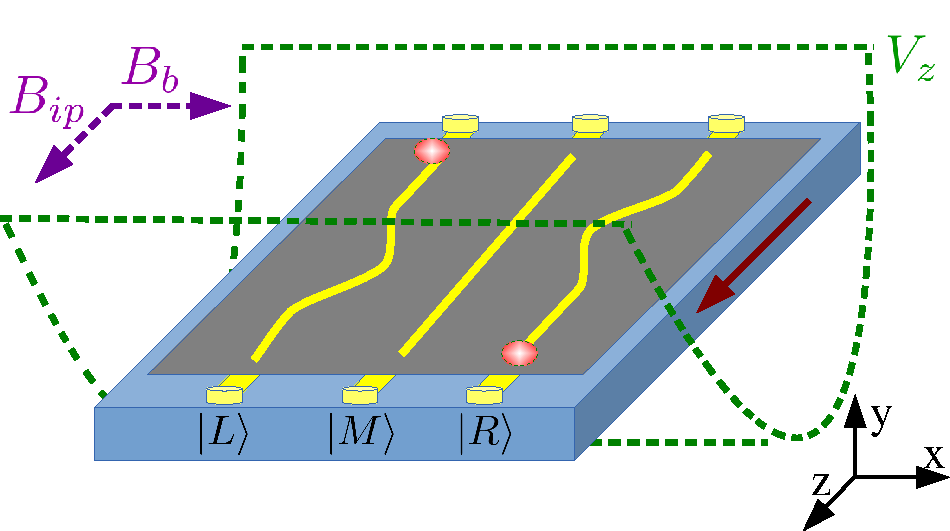
\includegraphics[width=\linewidth]{ch2_numerics/Schematic3.pdf}
  \caption{(Color online) Schematic of the suggested setup for observing the CTAP process in a system of waveguides. Note that the asymmetric approach of the outer wires to the middle wire is exaggerated, so that the counter-intuitive arrangement is visible. The atom is initially located in the left guide and, due to the presence of a harmonic oscillator potential $V_{z}$ in the $z$-direction, travels along the direction indicated by the red solid arrow. We also show the expected position of the atom at $t=\pi/{\omega_z}$ in the right hand side guide and indicate the orientation of the bias field, $B_b$, and the applied field, $B_{ip}$ (purple dashed arrows).}
  \label{fig:Schematic}
\end{figure}

Let us first briefly review the CTAP process by considering an atom trapped in a linear system of three
identical, one-dimensional microtraps \cite{Eckert:04}.  Assuming that the atom is in its centre-of-mass ground state in the trap on the left hand side,
$|L\rangle$, it can reach the ground states of the other two traps, $|M\rangle$ and $|R\rangle$, through coherent tunnelling described by the strength $J_{LM}$ for the transition $\vert L \rangle\to\vert M \rangle$ and $J_{MR}$ for $\vert M \rangle\to\vert R
\rangle$. In this basis the Hamiltonian is given by
\begin{equation}
  \label{eq:wgHamiltonian}
  H(t)=\hbar\begin{pmatrix}
                    0             & -J_{LM}(t) & 0  \\
                   -J_{LM}(t)  & 0            & -J_{MR}(t) \\
                    0             & -J_{MR}(t) & 0  
  \end{pmatrix} ,
\end{equation}
where the energy of the trap ground states was re-normalized to zero. The tunnelling strengths are assumed to be time-dependent, which can be achieved by increasing or decreasing the distances between neighbouring traps, $d_{LM}(t)$ and $d_{MR}(t)$. The eigenstates of the Hamiltonian \eqref{eq:wgHamiltonian} are well known \cite{Bergmann:98} and of particular interest for adiabatic transport is the so-called dark state
\begin{equation}
  |d\rangle=\cos\theta|L\rangle-\sin\theta|R\rangle,
\end{equation}
in which the  mixing angle $\theta$ is given as a function of the tunnelling strengths as
\begin{equation}
  \tan\theta=J_{LM}/J_{MR}.
\end{equation}
This state has a non-degenerate zero eigenvalue and an adiabatic evolution will therefore guarantee that the system, once prepared in
$|d\rangle$, will always stay in it. Note that the only contribution of $|M\rangle$ to $|d\rangle$ is through the mixing angle and that the system has zero probability to be found in $|M\rangle$ at any time.

The CTAP process can now be understood by considering an atom initially in the state $|L\rangle$. Increasing and decreasing $J_{MR}$
before $J_{LM}$, which is counter-intuitive to traditional tunnelling schemes, continuously decreases the population in state $|L\rangle$
and increases the population in state $|R\rangle$, leading to a 100\% transfer at the end of the process.

Adapting this process to a system of waveguides is now straightforward. The temporal dependence of the tunnelling strength in eq.~\eqref{eq:wgHamiltonian} can be replaced by a spatial one through suitable adjustment of the distance between neighbouring waveguides as a function of the direction the particle travels in (see Fig.~\ref{fig:Schematic} for a schematic view) \cite{Eckert:06}.

There are, however, several conditions that both, the microtrap and the waveguide system, must fulfil for the CTAP dynamics to occur. Firstly, the process must be adiabatic with respect to the other relevant energy scales in the system. For the waveguide system this means the whole process has to be slower than the inverse of the approximate transverse trapping frequencies of the guides. As typical numbers for such guides are in the kHz regime, this means that the time allowed for the atom to travel along the chip  can be much shorter than a typical system's lifetime. The second condition which has to be fulfilled, as previously mentioned, is that all trapping states are in resonance at any point in time, which is difficult to achieve once the potentials of the individual guides start to overlap. However, we will demonstrate in the next section how a waveguide setup on an atom chip is a realistic experimental system in which this resonance condition can be fulfilled to a good approximation.

\subsection{Atom Chips}
\label{sec:Atom Chips}

Atom chips are versatile experimental tools that are by today used extensively in experiments with ultra-cold atoms \cite{Folman:00,Fortagh:07}. A small current flowing through nano-fabricated wires on the substrate produces a magnetic field gradient in such a way, that cold atoms can be trapped very close to the surface. Because the layout of the nanowires can be chosen during the chip's production process, atom chips have been used in many cold atom experiments to produce microtraps, interferometers and waveguides \cite{Fortagh:07,Schwindt:05,Schumm:05,Petrovic:11}. Here we will take advantage of this versatility to consider waveguides in the geometry indicated in Fig.~\ref{fig:Schematic} and develop a procedure which will allow to observe high fidelity transport based on CTAP.

Let us briefly review the basic description and properties of atom chip trapping. The magnetic potential $\bf B$ at position $\bf r$ generated by a typical nanowire on an atom chip can be described by the Biot-Savart law
\begin{equation}
   {\bf B}= \frac{\mu_0 I}{4\pi} \oint \! \frac{d{\bf l}  \times {\bf{\hat r}}}{{r^2 }},
\end{equation}
where $I$ is the current in the wire, $\mu_0$ the vacuum permeability, $\bf{\hat r}$ the unit vector in the direction of $\bf r$ and $d{\bf l}$ is the differential length of the wire carrying current $I$. For this expression to be valid, however, we have to assume that the thickness of the wires is negligible, which is a good approximation as long as we are using the properties of the field at a sufficient distance above the chip's surface. To achieve this and to lift the field minima above the nanowires for the desired waveguide structure, a homogeneous magnetic bias field, $B_b$, can be applied orthogonal to the current flow. This raises the potential minimum to a height above the wire given by
\begin{equation}
  r_0=   \frac{\mu_0}{2 \pi} \frac{I}{B_b}.
\end{equation}
Finally, to lift the degeneracy of the spin states of the atoms and avoid losses due to spin flips at the centre of the waveguide a further magnetic field, $B_{ip}$, parallel to the direction of the wires is usually applied.

\begin{figure}
  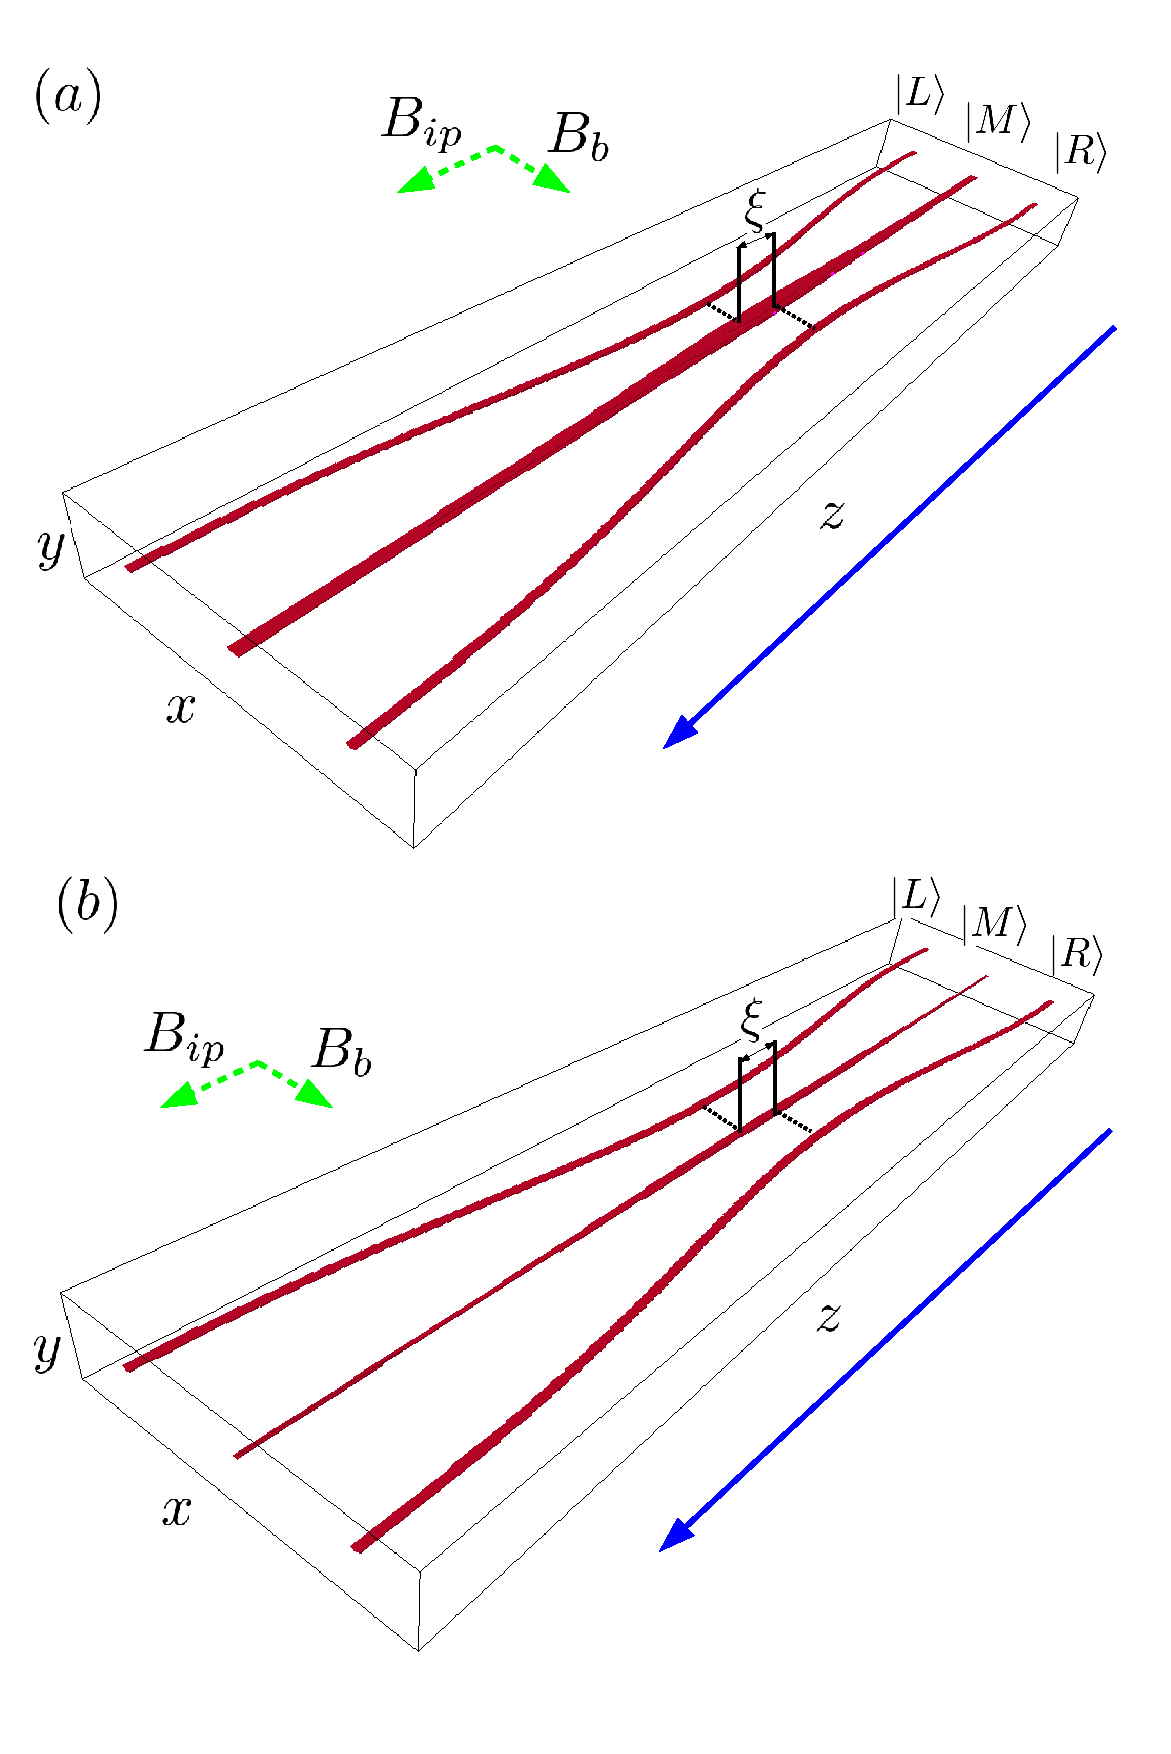
\includegraphics[width=\linewidth]{ch2_numerics/3D2.pdf}
  \caption{(Color online) Isosurfaces of the waveguides created on an atom chip with the direction of propagation indicated by the blue solid arrow (for clarity $V_z=0$ in this plot). The dimensions of the interesting area on the chip we simulate are $20\mu$m $\times 1000\mu$m ($x \times z$) and we take a height ($y$ direction) above the chip of $4\mu$m into account. The three wires are initially equally separated by $7\mu$m and their distance at the position of closest approach is $4.3\mu$m. The left wire remains straight initially for a distance of $50\mu$m, which produces an asymmetry in the point of closest approach of the left and right wires to the middle wire as indicated by $\xi$. The bias and applied fields (indicated by the green dashed arrows) are $B_b=140 \times 10^{-4}$T and $B_{ip}=300 \times 10^{-4} $T. In (a) the currents of the left, middle and right wires are $I_L=I_M=I_R=0.1$A respectively and in (b) the currents of the left and right wires are $I_L=I_R=0.1$A and the middle wire current is reduced to $I_M=0.07$A.}
      \label{fig:Potentials}
\end{figure}

\begin{figure}
  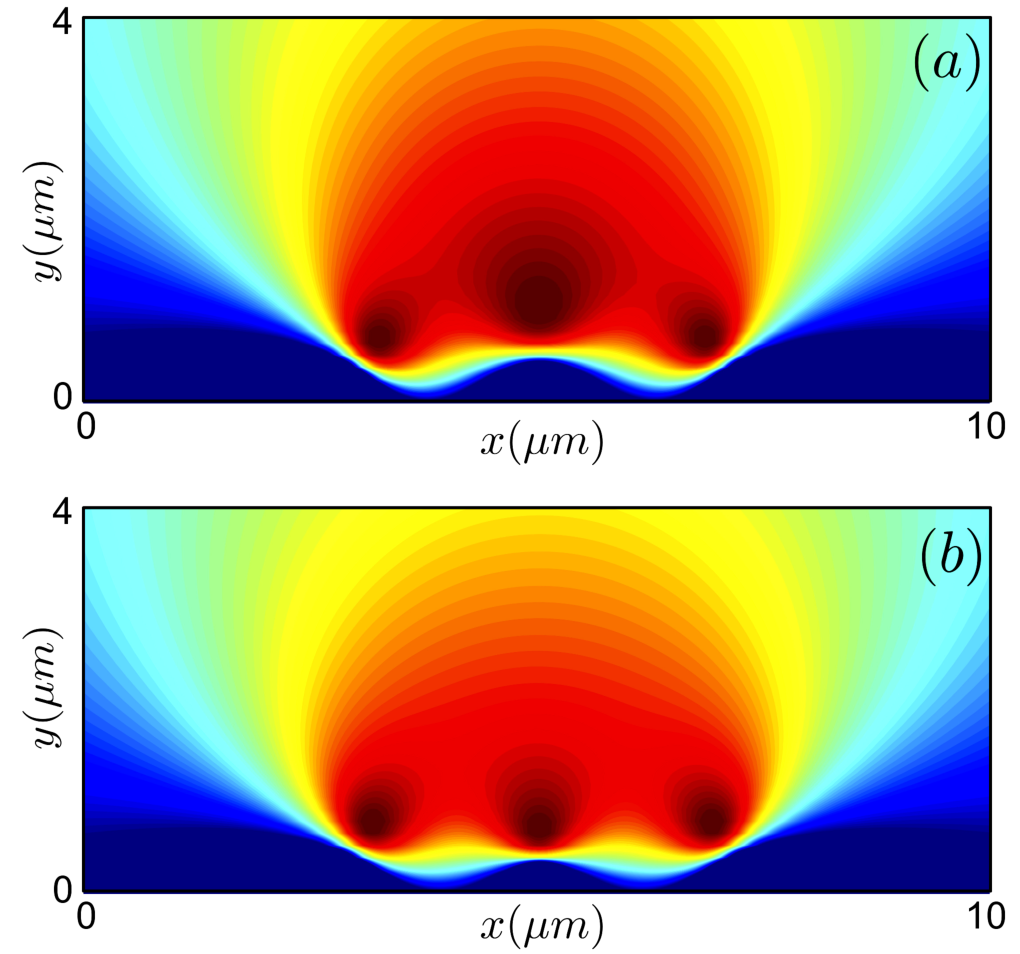
\includegraphics[width=\linewidth]{ch2_numerics/Central_slice_contrast.pdf}
  \caption{(Color online) Contour plot of the waveguides at 500$\mu m$ along the z-axis. Panel (a) shows the deformation of the waveguides when all currents are equal, $I_L=I_M=I_R=0.1$A and panel (b) shows how this effect can be mitigated by using a reduced middle wire current of $I_M=0.07$A, while the current in the outer wires remain at $I_L=I_R=0.1$A.}
  \label{fig:slice}
\end{figure}

An example of the waveguide potentials resulting from this model for $^6$Li  atoms and for experimentally realistic parameters is shown in Fig.~\ref{fig:Potentials}. If an atom is initially located in the left waveguide and travels in the positive $z$-direction, these waveguides provide the desired counter-intuitive tunnel coupling needed for CTAP. To give the atom momentum to travel along the wires we add an additional harmonic oscillator potential, $V_z$, of frequency $\omega_z$ along the $z$-direction, which is centred at the middle of the chip (see Fig.~\ref{fig:Schematic}). This will also lead to a re-focusing of the travelling wavepacket at the classical turning point on the other side of the chip and help to clearly determine the position of the atom.

To ensure that the process is adiabatic and the atom remains in the dark state of the system at all times, the total time for the process has to be much larger than the inverse of the transverse trapping frequencies of the individual waveguides. By approximating the potentials to have a harmonic oscillator shape in the transverse direction, we find the inverse of the relevant frequency to be of the order of $f_{HO} ^{-1}\approx 0.2$ ms and by choosing the trapping frequency of the harmonic oscillator in the z-direction to be $\omega_z=2 \pi \times 5$ Hz, the total time taken for the process (half an oscillation) is $0.1$ s. This allows to clearly fulfill the adiabaticity condition at any point during the evolution. 

Finally, the bend in the wires will lead to a potential from the currents in the $z$-direction, which requires the atom to have enough kinetic energy to overcome it and therefore sets an upper bound to the adiabaticity that can be reached. However, this effect can be reduced by increasing the length of the atom chip ($z$-direction) and therefore reducing the curvature of the wires. From our simulations, we find that the kinetic energy resulting from locating an atom initially at the edge of a chip that is $z_{max}=1000 \mu$m long allows us to successfully propagate the atom though the waveguides using the harmonic trap described above.

\subsection{MPI and CUDA}
\label{sec:MPICUDA}

To simulate the propagation of the atom along the waveguide we solve the three-dimensional time-dependent Schr\"odinger equation using the well known Fourier Split Operator method \cite{Fleck:splitop}. A typical numerical implementation of this method requires the use of 4 Fourier transforms followed by 3 complex multiplications for each time step. The numerical library we make use of to perform the Fourier transforms is the well known FFTW library, and its GPU implementation CUFFT \cite{Nvidia:cufft_4_1}.

Performing three dimensional Fourier transforms is the most intensive part of our code with the length of time required to perform one iteration of the split operator method depending heavily upon the size of the numerical grid. As discussed in the previous section, the atom chip has a relatively large extension in the $z$-direction  ($z_{max}=1000 \mu$m) compared to the other dimensions. Since the maximum value of the momentum grid is defined as $p_{max} = \frac{\pi N_z}{z_{max}}$ we require a large number of points, $N_z$, for our grid to be large enough to resolve the longitudinal momentum stemming from the external harmonic oscillator potential. This is the main reason that the computational resources required to simulate the system are quite substantial.

\subsubsection{GPU Computing}

To overcome the numerical barrier presented by this system we turn to the relatively new computing paradigm of GPU (graphics processing unit) computing. Whereas traditional computers perform computations using the central processing unit (CPU), GPU computing allows some of the work to be offloaded to the graphics processor. GPUs are inherently SIMD (single instruction, multiple data) devices, designed for operating upon a large data set at a given time with a single task, such as a 2D grid of pixels. Due to their parallel nature, GPUs can perform better than CPUs for certain types of calculations. One example where they offer large performance gains are fast Fourier transformations (FFTs) and it was recently shown that the Fourier split operator method can be accelerated using GPU computation \cite{Bauke:11}. This performance increase offers the numerical power needed to simulate the above system and we have implemented the algorithms for split-operator evolution of the Schr\"odinger equation with C, CUDA and Nvidia's CUFFT libraries for the Fourier transforms. 

\subsubsection{Performance}
To demonstrate the performance offered by GPU computing we compare it to using FFTW with MPI, a more traditional CPU-based method. The message passing interface (MPI) implementation allows the code to be run across multiple machines, benefiting from the parallelism which may be offered by a supercomputing cluster. Although MPI-enabled FFTW is fast and supports extremely large grid sizes, it requires computer-cluster access of a significant size to be a viable option. 

To effectively simulate the CTAP process and accurately resolve the momentum, our code requires a grid size of $256\times 64\times1024$ ($x\times y\times z$). For accurate time evolution a timestep of $\Delta t = 1\times 10^{-6}$ s was found to be adequate. For the GPU simulations, the test system was an Intel Core i7 2600K CPU at stock frequency, 8GB DDR3 memory operating at 1600 MHz, 7200 RPM HDD, Nvidia GeForce GTX 580 with 3GB of onboard memory running at 783 MHz GPU core frequency, 1566 MHz shader processor frequency, and 2010 MHz memory frequency. For all simulations the desktop was running Ubuntu 11.10 64-bit operating system and all calculations were performed in double precision (64-bit floating point) where applicable. For the CPU simulations we utilized the supercomputers at ICHEC (Irish Centre of High-End Computing).

Table \ref{tbl:timing} shows the approximate timings for the completion of runs on GPU and CPU. As one can see, not only does GPU computing offer a 6-fold improvement over a single CPU, it also allows us to achieve a performance level which is comparable to a 64 core CPU. Such performance has previously been restricted to high powered supercomputers. Having such computational power available to a single user on a Desktop computer allows us to obtain a large volume of simulated data on a much shorter timescale rather than through the use of a shared resource CPU-based computer cluster. Additionally, a second GPU card added to the system allowed concurrent runs of the code, which effectively halved the overall time required for a large number of simulations. It is also worth mentioning that moving computations over to the GPU of the system frees up the CPU and a large part of the system memory to be used for other task that would have previously been inhibited by CPU bound computations.

\begin{table}[tb]
  \begin{center}
    \begin{tabular}{|c||c|c|c|}
      \hline
      Device & Num. Devices & Timing  & Rel. Improvement \\ \hline
      CPU (MPI) & 8 & $\sim$6 Hr & 1.0$\times$ \\ 
      & 16 & $\sim$4 Hr & 1.5$\times$ \\
      & 32 & $\sim$1.5 Hr & 4.0$\times$ \\ 
      & 64 & $\sim$1 Hr & 6.0$\times$ \\ \hline
      GPU & 1 & $\sim$1 Hr & 6.0$\times$ \\ \hline
    \end{tabular}
  \end{center}
   \caption{The approximate times taken to simulate the propagation of an atom through our atom chip system on both GPU and CPU.}
   \label{tbl:timing}
\end{table}
     

\subsection{3D Simulations}
\label{sec:Results}
In the following section we will present a set of typical results from the GPU accelerated 3D simulations we have carried out over a large range of experimentally controllable parameters and show that the atom chip allows for the CTAP process to take place. All parameters for our atom chip are the same as in Fig.~\ref{fig:Potentials} unless otherwise stated.

Our simulations start out with a single $^{6}$Li atom which is initially located in the left waveguide. Its transversal wavefunction corresponds to the ground state of the potential in the transversal direction (determined numerically) and longitudinally we assume a Gaussian profile of similar width. We then evolve this initial state in time and due to the longitudinal harmonic oscillator potential centred at the middle of the atom chip ($z=500 \mu$m), the atom starts to propagate along the waveguide. 

Initially the wires are far enough away from each other for each waveguide to be approximately given by the current of the wire closest to it and if all currents are identical, the waveguides are in resonance. However, once the wires start approaching each other, the respective magnetic fields add and create waveguide potentials of unequal size (see Figs.~\ref{fig:Potentials} (a) and \ref{fig:slice} (a)). This drives the transversal ground states of the guides out of resonance and the conditions for observing the CTAP process are no longer given.
 
However, atom chips offer an intriguingly straightforward way to adjust for this, as the current in each wire can be individually (and even time-dependently) controlled. This can be used to compensate for effects stemming from the potentials overlapping and ensure resonance between the waveguides \cite{OSullivan:10}. While one can imagine a numerically optimised algorithm that adjusts the currents in a time-dependent manner based on the position of the centre-of-mass of the atom, here we will show that a much simpler approach, which maintains the simplicity of all currents being constant in time, is already sufficient. We suggest to reduce the current in the middle wire so that in the crucial coupling region, where the magnetic fields from neighbouring waveguides have the strongest influence on each other, the waveguides are approximately resonant. 

To demonstrate the effect of this adjustment we show in Fig.~\ref{fig:slice} a transversal cut through the system at the middle of the chip ($z=500 \mu$m) for the case where (a) all three currents are identical ($I=0.1$A) and (b) where the current in the middle wire is reduced ($I_M=0.07$A). One can clearly see that the transversal shape of the waveguides is very similar for the case of the reduced centre current, which indicates that this approach can lead to enhanced resonance between the guides.

In the areas where the guides are further away from each other, however, the reduced current in the middle wire will have the opposite effect and reduce the quality of the resonance. This can clearly be seen from the iso-potential surface plot in Fig.~\ref{fig:Potentials} (b). Yet, since the tunnelling in these areas is small, it has only a negligible influence on the CTAP process and we will in the following demonstrate that the near resonant setup of Fig.~\ref{fig:slice} (b) allows to observe the CTAP process. 

In Fig.~\ref{fig:Populations} we show the population in each waveguide as a function of time for an atom chip with reduced current in the central wire. The results in Fig.~\ref{fig:Populations} (a) are obtained for the situations where the wires are arranged such that the counterintuitive tunnelling sequence takes place and full transfer from the initial guide into the final guide is clearly visible. Only a small population in the central guide appears halfway through the process, and while the ideal CTAP process does not allow for population in the central trap at any time, the limited adiabaticity and resonance of the simulated setup leads to this temporary deviation. However, it has no effect on the final state.

In contrast to this, and confirming that the large fidelity of the transport process above is due to CTAP, we show in Fig.~\ref{fig:Populations} (b) the results for an intuitive arrangement of the waveguides on the atom chip. As is clearly visible, this does not produce high fidelity population transfer to the guide on the right hand side, but rather leads to a split of the probability between the middle and the right hand side wire. 

\begin{figure}[tb]
  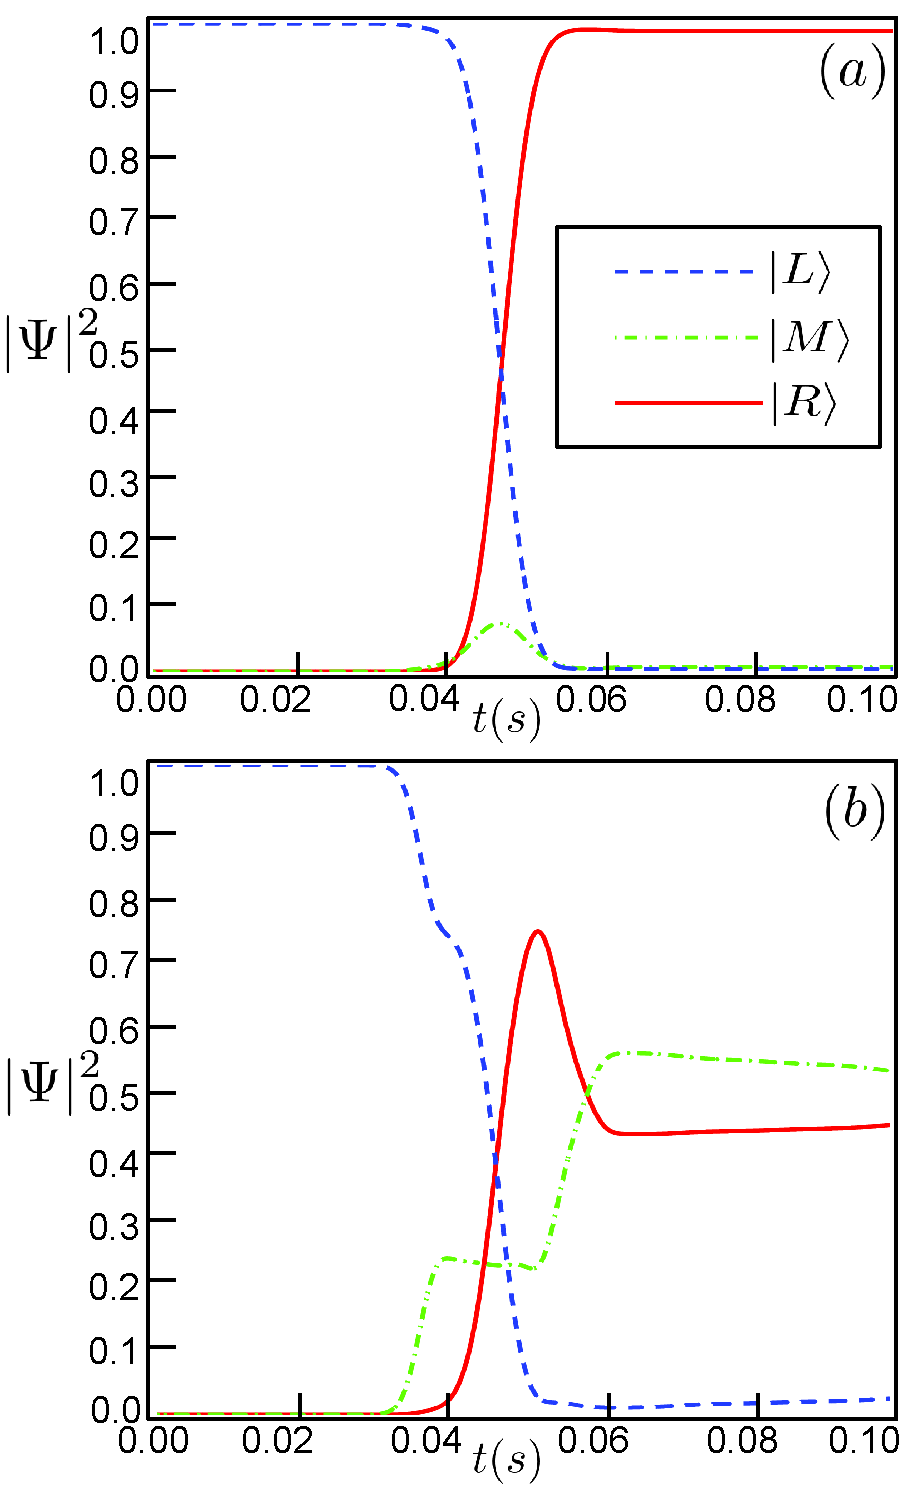
\includegraphics[width=\linewidth]{ch2_numerics/Populations.pdf}
  \caption{(Color online) The population in the left (blue dashed line), middle (green dot-dash line) and right (red solid line) waveguides as a function of time for (a) the counter-intuitive waveguide arrangement and (b) for intuitive, direct tunnelling one. The current in the middle wire is reduced to $I_M=0.07 A$.}
  \label{fig:Populations}
\end{figure}

While Fig.~\ref{fig:Populations} only gives an indication of the ongoing process as a function of time, the presence of the CTAP process for the counter-intuitively arranged wires can also be inferred from looking at the atomic probability distribution in real space. For this we show in Fig.~\ref{fig:Pcolor}  the density of the atomic state in the $x$ and $z$ plane at $t=0.048$ s integrated over the $y$-direction. At this time the atomic wavepacket is in the region where the tunnelling interaction between all three waveguides is large and clear differences between the two situations are visible. Fig.~\ref{fig:Pcolor} (a) shows the counter-intuitive situation where the wavepacket can be seen to follows the dark state with only a negligible population component in the middle waveguide. In contrast, Fig.~\ref{fig:Pcolor} (b) shows the intuitive setup, in which the population is distributed between all three waveguides and clear signatures of Rabi oscillations due to the direct tunnelling are clearly visible.

\begin{figure}[tb]
  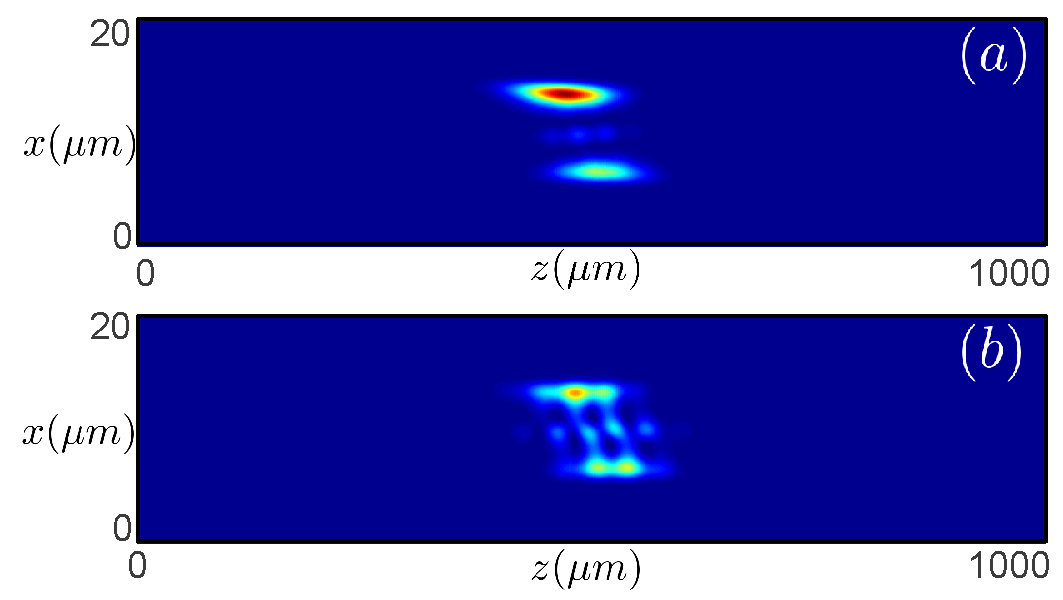
\includegraphics[width=\linewidth]{ch2_numerics/Pcolor.pdf}
  \caption{(Color online) The density of the atomic state at $t=0.048$ for (a) the counter-intuitive setup and (b) the intuitive one. The current in the middle wire is $I_M=0.07$ A in both cases.}
  \label{fig:Pcolor}
\end{figure}

It is exactly these Rabi oscillations in the intuitive process that lead to the time-dependence of the final population in each waveguide and therefore a strong dependence of the outcome on small changes in the system parameters. This can be seen when examining Fig.~\ref{fig:Current}, where we show the final population in the right hand side waveguide as a function of the current in the middle wire $I_M$. For the intuitive process (blue line), the final population varies significantly with changing $I_M$, whereas the counter-intuitive setup (red line) is very robust to these changes, with the fidelity of population transfer never dropping below $0.98$. This is another indication that the transfer is due to CTAP. 

\begin{figure}[tbh]
  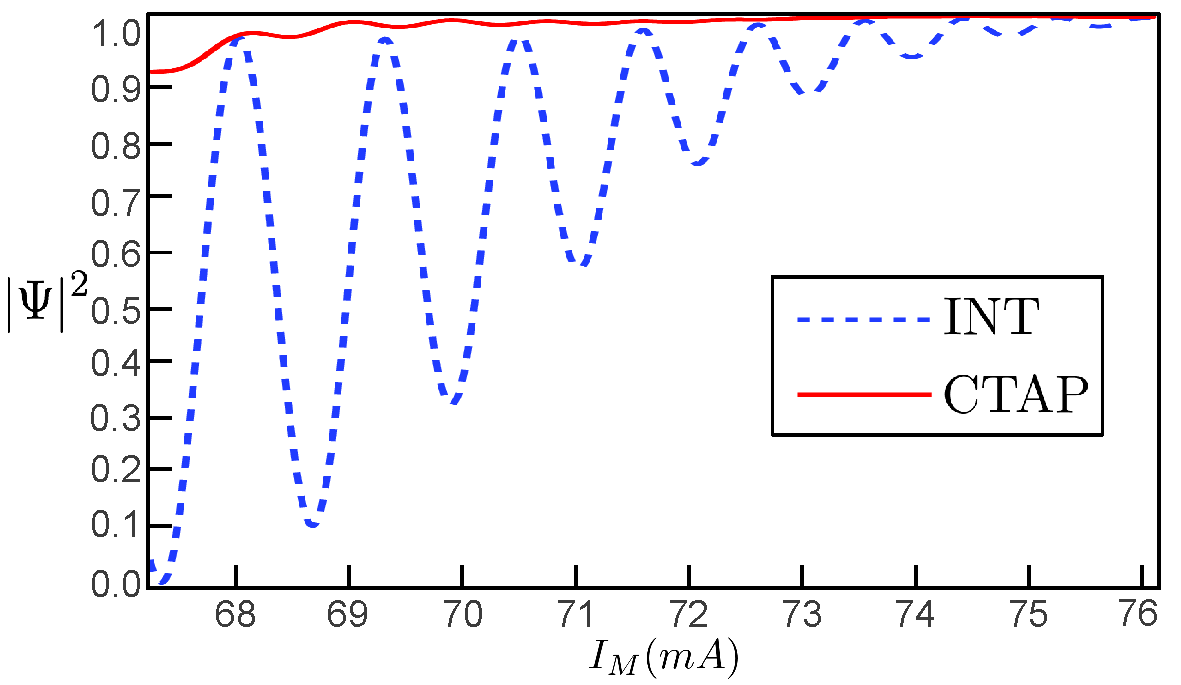
\includegraphics[width=\linewidth]{ch2_numerics/Current_3.pdf}
  \caption{(Color online) The final population in the  target waveguide for both the CTAP (red solid line) and intuitive (blue dashed line) processes, for values of $I_M=0.0672$A to $I_M=0.0761$ A in steps of $0.001$ A.}
  \label{fig:Current}
\end{figure}

From Fig.~\ref{fig:Current} it is also clear that, while there are large oscillations in the fidelity of the intuitive process, there is an upward trend in the fidelity of the process towards unity as the current in the middle wire increases. However, at these higher values of the middle wire current, the waveguides are no longer resonant at all times and one would expect that neither the CTAP nor the intuitive processes would lead to high fidelity transfer. Nevertheless, the simulations show that this is not the case.

We conjecture that in the regime of larger currents in the middle wire the population transfer is due to  Stark-shift-chirped rapid-adiabatic-passage (SCRAP) \cite{Bergmann:05}. In this process a time-depend shift of the energy of the intermediate state in the traditional three-level arrangement allows for high-fidelity population transfer  between two states, independent of being in the intuitive or counter-intuitive situation. A translation of this to the spatial realm is straightforward: the approach and retreat of the outer wires from the middle one shift the energy of the central waveguide in a spatially dependent manner. This effect is the topic of a future investigation. 
\subsection{Conclusions}
\label{sec:Conclusions}

We have performed fully three dimensional simulations of an experimentally realistic waveguide system on an atom chip, where the arrangements of the wires produce spatial dependent tunnel-couplings between the waveguides. These simulations were done by implementing the CUFFT library provided by Nvidia, which made this problem numerically tractable on a desktop computer. 

Using a simple method for controlling the resonance as the waveguides are brought close together, we have demonstrated that  a counter-intuitive approach of the outer wires to the middle allows to observe high fidelity and robust transfer between the wires due to CTAP. In contrast, for intuitively coupled waveguides, where direct tunnelling between them is allowed to occur, significant Rabi oscillations between all guides exist. This makes the transfer process highly sensitive to the system parameters. While a large number of theoretical works on CTAP exist, the analysis presented offers a direct way for experimental observation and confirmation of the effect.

Finally, we have also seen a first indication that waveguide systems might be natural systems to observe the  SCRAP protocol and a detailed investigation will be the topic of a future work. While we have used the numerical methods described here to perform three dimensional simulations, they can actually be used in any number of dimensions, where they still offer large performance gains over standard CPU approaches. 

\subsection{Acknowledgements} 
The authors would like to thank Peter Kr\"uger and Thomas Fernholz for valuable discussions and ICHEC for use of their computing resources for the MPI-enabled code. This work was supported by Science Foundation Ireland under project number 10/IN.1/I2979.


\fi
%%%%%%%%%%%%%%%%%%%%%%%%%%%%%%%%%%%%%%
\newif\ifvtxdyn
\ifvtxdyn
    \chapter{Vortex dynamics}
        \section{Vortex lattice}

    \fi
%%%%%%%%%%%%%%%%%%%%%%%%%%%%%%%%%%%%%%
\newif\ifmoire
\moiretrue
\ifmoire
    \chapter{Moir\'e superlattice structures}
        \section{Delta-kick dynamics}
The use of delta-kicked Hamiltonians are widespread in the study of chaotic systems [citation]. The delta-kicked rotor is a prime example of such a system that exhibits chaotic motion following a series of successive kicks.

Another such model, building upon the kicked rotor, is the kicked harmonic oscillator, wherein the Hamiltonian acquires an additional quadratic potential. The behaviour of such systems have been studied [], and are interesting to understand the onset of chaos in both classical and quantum mechanical systems. By converting the conjugate variables to quantum operators, the quantum mechanical analogues can be examined. Granted, chaos in the quantum mechanical world differs from that of the classical world (e.g. the existence of quantum unitary evolution), insights may be gained from the study of systems on the boundary between the quantum and classical world.

Here I propose such a system, given a rapidly Bose-Einstein condensate featuring a well ordered vortex lattice. The goal is to generate chaotic motion of the vortices in the condensate through kicking with an optical lattice that with a period given by the rotation and translational symmetry of the vortex lattice. Since we know the vortex lattice is an Abrikosov lattice with 6-fold symmetry, we can say that given a rotation frequency of $\Omega$, the lattice will return to the same orientation after a rotation of $\Omega/6$. Thus, we can kick the system at this interval with a stationary optical lattice potential, without the need to rotate with the system, making this more experimentally realistic.


For the purpose of this work the standard single component Bose--Einstein condensate in a radially symmetric trap of frequency $\omega_\perp$ was assumed. By tightly confining the condensate along the $z$-dimension, with trapping frequency $\omega_z$, such that $\omega_z >> \omega_\perp$, the condensate attains a pancake-shaped geometry. Since the energy required to excite any higher modes along $z$ is $\hbar\omega_z$, we can assume all excitations are planar along the radial coordinate $x-y$ axes. Modelling of this system is performed in the  mean-field limit, given by the Gross--Pitaevskii equation, with Hamiltonian

\begin{equation}\label{eqn:gpe_h0}
	H_{\mathrm{GP}} = -\frac{\hbar^2}{2m}\nabla^2 + \frac{1}{2}m\omega\perp^2\mathbf{r}^2 + g\vert\Psi(\mathbf{r},t)\vert^2.
\end{equation}

Here $g$ describes the interaction between atoms in the condensate, and is given by \begin{equation}
g = \frac{4\pi\hbar^2a_s}{m}
\end{equation},
where $a_s$ is the s-wave scattering length of the atomic species. Restricting the system to a two-dimensional geometry also requires the move to an effective interaction which encompasses the net effect of the integrated $z$-dimension. This is enabled by scaling the interaction by the length of the harmonic oscillator along the $z$-dimension, and becomes
\begin{equation}
g_{2D} = g\sqrt{\frac{m\omega_\perp}{2\pi\hbar}}.
\end{equation}

To generate vortices in the condensate angular momentum must be added to the system. Experiemetnally, this can be achieved by stirring the condensate with a blue-detuned beam [], by carefully inverting the trapping potential [], or through use of artificial gauge fields [], to name a few. Numerically, this is achieved by assuming that we are in the co-rotating frame with the condensate, and accounted for by addition of an angular momentum operator along $z$ scaled by rotation frequency, $\Omega L_z$ to the Hamiltonian. The time dependent nature of the system can be analysed using the form

\begin{equation}\label{eqn:gpe}
	i\hbar\frac{\partial}{\partial t}\Psi(\mathbf{r},t) = \left[ H_{\text{GP}}  -  \Omega_z L_z \right] \Psi(\mathbf{r},t),
\end{equation}
where $\Omega_z$ is the angular frequency about the $z$-axis and $L_z = xp_y - yp_x$ is the angular momentum operator. If the angular rotation frequency approaches the condensate trapping frequency, $\Omega \approx \omega_\perp$ the condensate gains a large triangular lattice of vortices. Assuming an upper limit frequency of $\Omega = 0.995\omega_\perp$ allows the system to have a very large vortex lattice, and still be described capably by mean-field theory. Further increases in the rotation frequency would allow the condensate to enter into a strongly correlated regime, and no longer be described using Gross--Pitaveskii theory.

As we are interested in lattice ordering effects, the assumption that the trapping frequency along the $z$-axis, $\omega_z$, is be much larger than the one along the transverse axis, $\omega_\perp$,  allowing the condensate to enter a pancake-shaped geometry is valid~\cite{BEC:Fetter_revmodphys_2009}. Neglecting the $z$ dimension ($\textbf{r}\equiv [x,y]$) simplifies the analysis of the system and resulting dynamics. For this work eq.~\eqref{eqn:gpe} will be numerically solved, using the pseudospectral Fourier split operator method making use of GPU computing\cite{NUMERICS}. For realistic experimental parameters I assumed  $N=4.9\times 10^5$ atoms of $^{87}$Rb, with an s-wave scattering length of $a_s=4.76\times10^{-9}$ m~\cite{BEC:Roberts_prl_1998}.

The numerically evaluated ground-state for the given set of parameters is shown in Fig.~\ref{fig:vlatt_gnd}, and it can be characterised by the filling factor (or filling fraction) $\nu=N/N_v$, i.e.~the ratio of atoms to vortices~\cite{BEC:Fetter_revmodphys_2009}. Values of $10 \leq \nu \leq 1000$ enter the so-called ``mean-field quantum Hall'' regime, with Gross-Pitaevskii theory working well. For values $\nu \leq 10$ the system is said to be strongly correlated. For the chosen parameters, the number of vortices within the visible density region is approximately 600, giving a filling factor of $\nu \approx 800 $. This places the system within the mean-field quantum Hall regime, and therefore a description using Gross--Pitaevskii theory is adequate~\cite{Vtx:Schweikhard_prl_2004}

\begin{figure}[tb]
    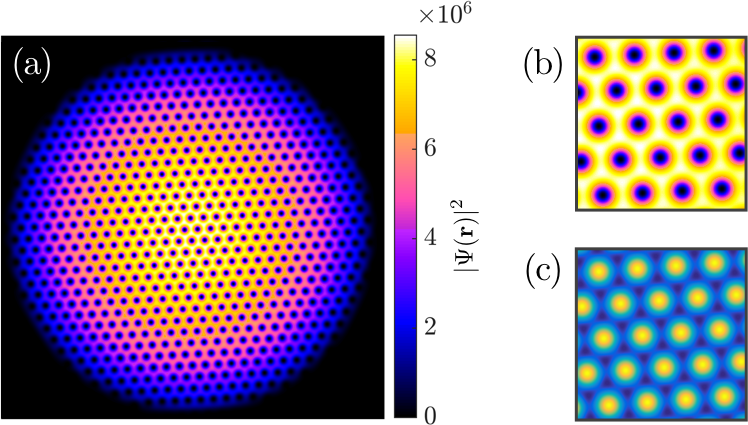
\includegraphics[width=0.5\textwidth, angle=0, trim=0 0 0 0]{ch4_kickit/fig1}
    \caption{(a) Vortex lattice ground-state in a harmonic trap with $\omega_\perp=2\pi$ s$^{-1}$ and rotating at $\Omega=0.995\omega_\perp$. This plot shows a condensate with a diameter of approximately $580~\mu\textrm{m}$; (b) Zoom in of vortex lattice at central density; (c) Optical lattice potential with a periodicity matching that of the vortex lattice.}
    \label{fig:vlatt_gnd}
\end{figure}

Given the large number of vortices in the condesate density, as well as the lowered density resulting from large centrifugal forces, the vortex cores become large and form a highly periodic triangular lattice. The non-orthogonal lattice vectors are given in $\mathbf{r}$-space by $\mathbf{a}_1 = a_v\{1,0\}$ and $\mathbf{a}_2 = a_v\{-1/2, \sqrt{3}/2\}$, where $a_v$ is the distance between vortex cores. The lattice constant is truly only constant in areas of near uniform density. Thus, due to the inhomogeneous wavefunction density, the vortices near the edges are separated by a much greater distance than those at the centre. For my analysis I have chosen to ignore all vortices near the condensate edge. The momentum space ($\mathbf{k}$-space) lattice vectors reciprocal to the given $\mathbf{r}$-space vectors are $\mathbf{b}_1 = 4\pi/(\sqrt{3}a_v)\{\sqrt{3}/2,1/2\}$ and $\mathbf{b}_2 = (4\pi/(\sqrt{3}a_v))\{0,1\}$.

Using an optical potential we can create a perturbation in the condensate density by switching it on for a brief period of time. Such a {\it kick} must occur only for a time much shorter than the rotation period of the vortex lattice, $\Omega = 0.995\omega_\perp$. For the work carried out herein, the time of the kick was given by $\tau_{\text{kick}}=10^{-5}$~s. This ensured that the vortex lattice was essentially stationary relative during the kick. To examine the effect that periodicity plays on the system, the optical potential was chosen to match the structure of the Abrikosov vortex lattice, with the angle of relative rotation $\theta_\Delta$ given as a free parameter. The optical potential was modeled as the sum of counter-propagating laser beams, as
\begin{equation}
    V_{\text{opt}} = V_0\displaystyle\sum_{j}\cos^2 \left[ \textbf{k}_{j}\cdot\textbf{r} \right],
\end{equation}
where $V_0$ is the optical lattice potential amplitude, and $j=\lbrace 0,1,2,\ldots \rbrace$ is the index of each respective laser with a differing $\mathbf{k}$-space wave-vector. By careful choice of the wave-vectors $\textbf{k}_{j}$ we match the density modulation given by the vortices to the optical potential. This is achieved using the reciprocal lattice vectors defined by the vortex lattice, $\mathbf{b}_{1,2}$, and an additional third wave-vector, $\mathbf{k}_3 = 4\pi/(\sqrt{3}a_o)\{\sqrt{3}/2,-1/2\}$. The lattice constant of the resulting potential is based on the optical intensity to match that of the vortex lattice.


Given that the vortex lattice constant in a rapidly rotating atomic BEC is large, optical lattices with wavelengths on the order of tens of microns are necessary \cite{BEC:Fallani_optexp_2005,BEC:Williams_optexp_2008}. By ensuring a short kick with an amplitude on the order of $10^{-2} \mu $, with $\mu$ as the BEC chemical potential, the result of the kick is an imprinted phase on the wavefunction (see Fig. \cite[find from images]) \cite{Vtx:Dobrek_pra_1999}. This leads to the development of a flow from the origin of each optical lattice potential maxima positions. As I will describe next, this in turn creates well-defined interference patterns resulting from phonons created by the kick. In the presence of a vortex lattice with a periodic core arrangement, this creates moir\'e superlattice structures \cite{mor:murata_acsn_2010} in the density of the condensate. Although this type of pattern has been observed in many solid-state systems, such as graphene on hexagonal boron nitride~\cite{nphys2272}, they appear to be static in such cases. In this system, the structures are dynamical, and revive at well defined intervals.

To study these resulting structures, I performed a spectral decomposition of the kinetic energy of the condesate~\cite{CT:Nore_prl_1997,CT:Nore_pof_1997,CT:Bradley_prx_2012}. To perform this, the wavefunction is first written in amplitude (density) $\rho(\mathbf{r},t)$ and phase $S(\mathbf{r},t)$ form via a Madelung transform, as
$
		\Psi(\mathbf{r},t) = \sqrt{\rho(\mathbf{r},t)}\exp{\left[\mathrm{i}S(\mathbf{r},t)\right]}.
$
Making use of the Gross-Pitaevskii energy functional \ref{eqn:gpe_functional}, and substituting in the above form gives
\begin{equation}
    E_{\text{kqp}} = \int d\mathbf{r} \left( \frac{\hbar^2}{2m}| \nabla\sqrt{\rho(\mathbf{r},t)} |^2  + \frac{m}{2}|\sqrt{\rho(\mathbf{r},t)}\mathbf{v}(\mathbf{r},t) |^2\right).
\end{equation}
One can decompose this into the quantum pressure (first) and kinetic energy (second) terms. The kinetic energy term can seen as a density-weighted velocity field via $\mathbf{u}(\mathbf{r},t) = \sqrt{\rho(\mathbf{r},t)}\mathbf{v}(\mathbf{r},t)$. This can be further decomposed into the sum of compressible and incompressible terms,
\begin{equation}
    \mathbf{u(r},t) = \mathbf{u}^c(\mathbf{r},t) + \mathbf{u}^i(\mathbf{r},t),
\end{equation}
where $u^c, u^i$ are the compressible and incompressible terms respectively. These can be solved by assuming  $\nabla \times \mathbf{u}^c(\mathbf{r},t) = 0$, and $\nabla \cdot \mathbf{u}^i(\mathbf{r},t) = 0$. This decomposition separates the energy contribution from phonons and vortex cores, representing compressible and incompressible terms respectively~\cite{CT:Horng_pra_2009}. By averaging over binned shells in $\mathbf{k}$-space, the kinetic energy spectra, $E^{c,i}(k)$, are calculated as~\cite{CT:Bradley_prx_2012}
\begin{equation}
	E^{c,i}(k) = \frac{mk}{2}\sum\limits_{j\in\mathbf{r}} \int\limits_{0}^{2\pi}d\phi_k \frac{ |\mathcal{U}_j^{c,i}(\mathbf{k},t) |^2}{s_k},
\end{equation}
where
\begin{equation}
	\mathcal{U}_j^{c,i}(\mathbf{k},t) = \int d^2 \mathbf{r} e^{-i(\mathbf{k}\cdot\mathbf{r})} u_j^{c,i}(\mathbf{r},t).
\end{equation}
The terms $u_j^{c,i}(\mathbf{r},t)$ represent the position-space kinetic energy components in the specified shell, where $\phi_k$ is the polar angle, and $s_k$ is the number of values in the chosen shell.

For a rapidly rotating vortex lattice carrying condensate, calculating the spectra via the above method returns quantities which closely resemble those used in classical fluids, investigating the onset of turbulence[citation]. Such figures can be seen in Fig [give a figure]. However, [Bradley et al??] have discussed how this method does not truly represent the kinetic energy of the system, due to [something with the kinetic spectrum I dont recall]. They propose a quantum version of the above description, which involves including the condensate phase, alongside the density weighted velocity field, as $\mathbf{u}(\mathbf{r},t) = \sqrt{\rho(\mathbf{r},t)}\mathbf{v}(\mathbf{r},t)\exp\left(iS(\mathbf{r},t)\right)$. The resulting kinetic spectra may accurately resemble the spectrum of the condensate in experimental work, however, the structure observed in the classical case is lost (see fig[include figure]). The effect kicking has can be observed in the compressible spectrum in both cases, but the periodicity is lost in the averaging. Thus, the work described will use the ``classical'' method herein.

\section{Dynamics following a kick}\label{sec:kickvl}
\subsection{Non-rotating condensate}
To fully characterise the effect kicking has on a rapidly rotating BEC carrying a vortex lattice it is instructive to understand the dynamics following a kick in the absence of a vortex lattice. For an accurate comparison, the trapping frequency of the non-rotating condensate is adjusted such that the background densities match that of the rotating condensate. This is achieved by assuming the centrifugal term competing against the harmonic oscillator frequency as $V_{\text{opt}} = 1/2m(\omega^2_\perp - \Omega^2)\mathbf
{r}$, where $Omega=0.995\omega_\perp$ is the value chosen for the rapidly rotating case.

###

For a stationary (non-kicked) condensate the kinetic energy spectrum will remain constant during time-evolution, with a kick leading to the appearance of new, time varying components. To observe this I numerically evolve the system by setting $V(\mathbf{r},t) = V_{\text{ext}}(\mathbf{r}) + V_{\text{opt}}(\mathbf{r},t)$, where the time dependent optical potential is only active for $\tau=10^{-5}$~s of the simulation time. As discussed earlier, this short kicking duration is sufficient to allow a phase imprint onto the condensate wavefunction, without any change in the density on the timescales of the kick itself. Next, I examine the compressible kinetic energy spectrum following the kick (see Fig.~\ref{fig:ekc_eki_novtx}). Unsurprisingly, the spectrum is dominated by a peak corresponding to the wave-vector associated with the optical potential at $k=4\pi/(\sqrt{3}a_o)$, and several smaller ones corresponding to its higher harmonics and higher harmonics of next nearest neighbour components of the lattice. This makes sense as nearest neighbour lattice spacings should be the dominant structure with higher order spacings dropping in intensity due to the limited system size. As no rotation is added by the imparted phonon modes, the incompressible energy is negligible compared to the scale of the compressible energy (see Figure~\ref{show incomp vs comp}), and thus I will restrict the analysis to the compressible part of the spectrum.

\begin{figure}[tb]
    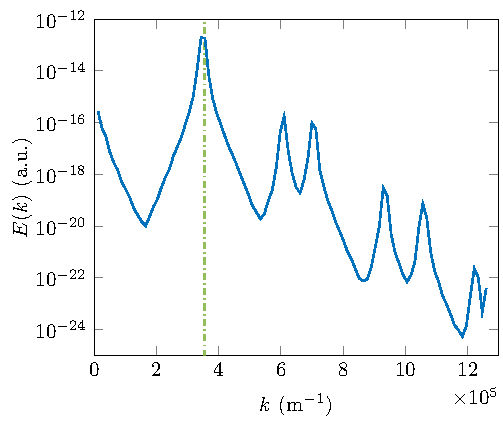
\includegraphics[width=0.48\textwidth]{ch4_kickit/fig2}
    \caption{Compressible energy spectrum of a non-rotating condensate directly following a kick. A peak at $k=4\pi/(\sqrt{3}a_o)$ can be seen, which corresponds to the lattice spacing, $a_o$ (indicated by the dashed line), and the smaller, higher energy peaks can be attributed to higher harmonics between nearest and next-nearest neighbours.}
    \label{fig:ekc_eki_novtx}
\end{figure}


%######################################################%#################################################################################%############################################################################################################
%               PAPER to be modified
%######################################################%#################################################################################%############################################################################################################

The evolution of the nearest neighbour peak in the compressible kinetic energy spectrum during the first 250 ms after the kick is shown in Fig.~\ref{fig:novtx_p5k}(a). It initially oscillates in and out of existence and eventually disperses over a wide range of wave-numbers. Snapshots of the density evolution are shown in Fig.~\ref{fig:novtx_p5k}(b), which clearly show that the oscillations correspond to the existence of a transient lattice pattern with several revivals, which have the same underlying structure as the optical potential. In fact, the lattice pattern is best formed whenever the main peak in the kinetic energy spectrum goes to zero, i.e.~when the imprinted kinetic energy has been converted into density modulations. The period of the oscillations can be related to the speed of sound divided by the lattice constant and therefore the appearance of the lattice can be attributed to phonon interferences.


\begin{figure}[tb]
	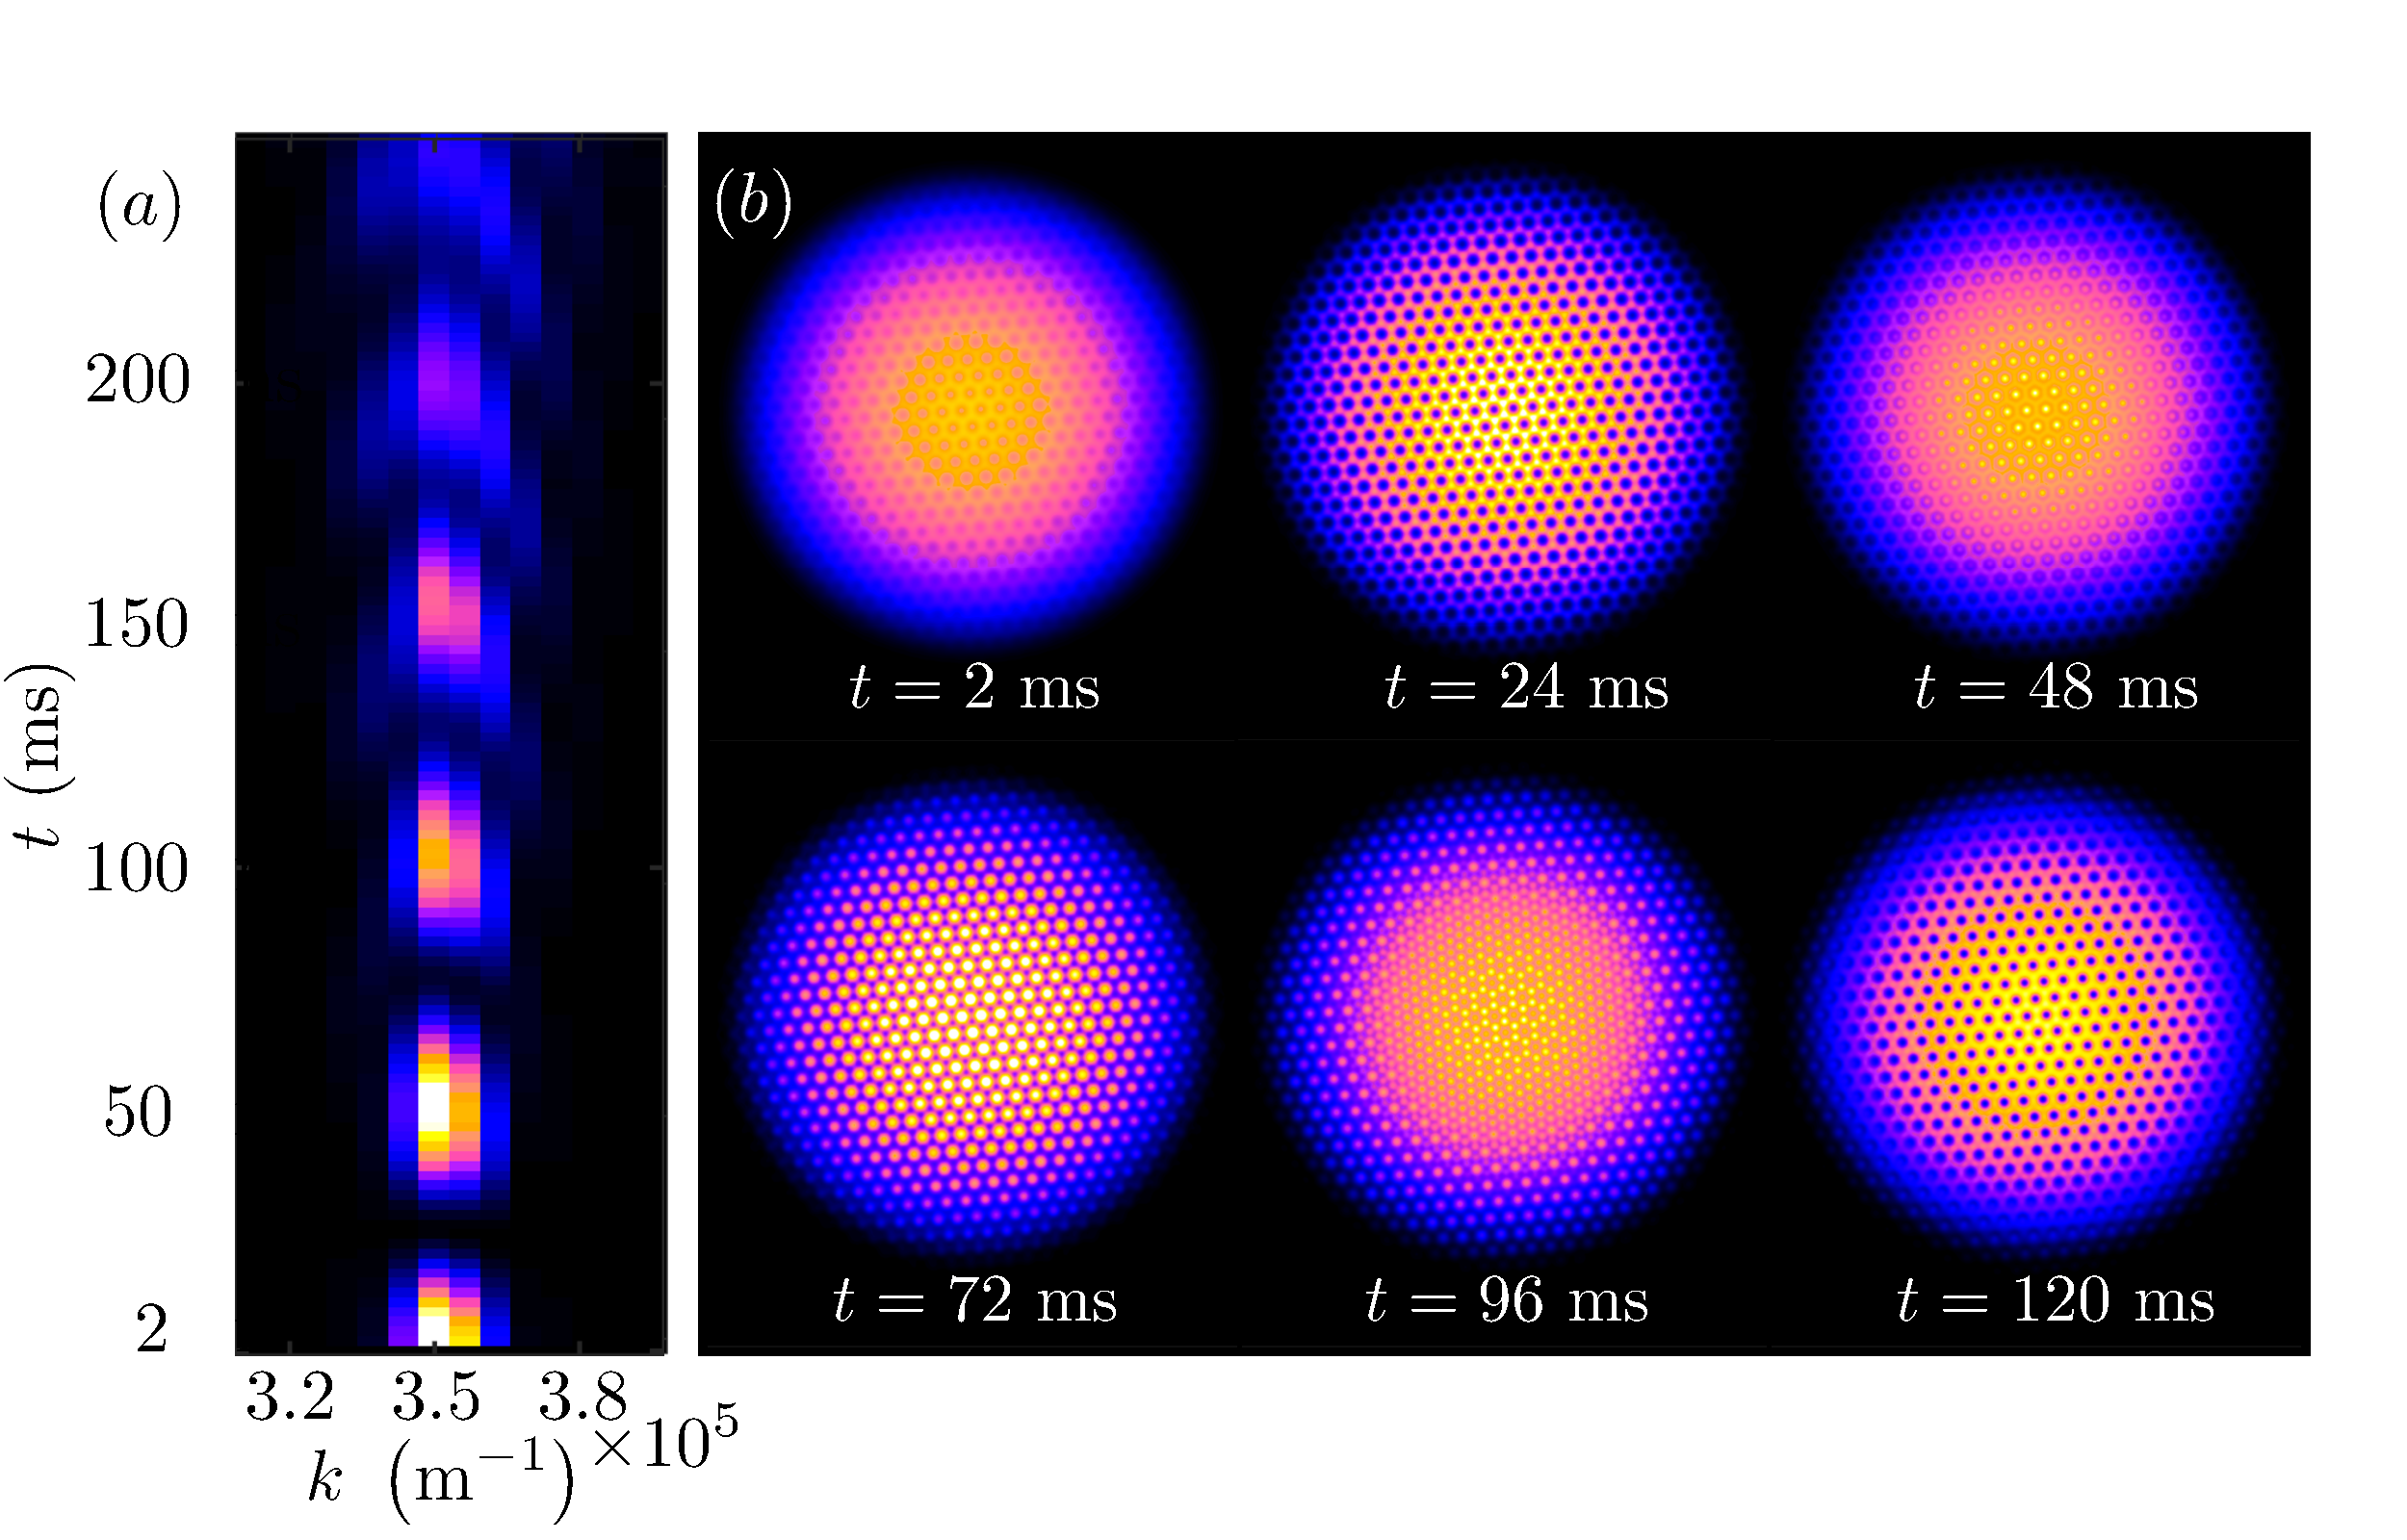
\includegraphics[width=0.48\textwidth]{ch4_kickit/fig3}
	\caption{(a) Main peak of the compressible kinetic energy spectrum for a kicking strength of $V_0 \approx 1.35\times10^{-2}\mu$. It can be seen to revive, and eventually disperse over a wide range of wave-numbers.  (b) Condensate densities at several times during the evolution. A pattern matching the optical potential can be observed to appear and disappear several times over the course of the evolution.}
	\label{fig:novtx_p5k}
\end{figure}


%######################################################%#################################################################################%############################################################################################################
\subsection{Rapidly rotating condensate}

    Kicking a condensate carrying an Abrikosov vortex lattice with the above optical lattice gives an additional parameter, $\theta_\Delta$, which describes the orientation of the imprinted phonon lattice angle relative to the vortex lattice. For simplicity, it is assumed that the vortex and optical potential lattices have the same lattice constant, $a_v=a_o=a$ (see below for a discussion of the incommensurate case), which means that symmetry allows us to restrict the angle to $\theta_\Delta\in[0,\pi/3]$. In the following it can be seen that adjusting $\theta_\Delta$ leads to the appearance of different, transient super-structures in the condensate density.

    If $\theta_\Delta=0$ (see Fig.~\ref{fig:moire_density}(a)) the kicking imparts kinetic energy at wave-numbers that are already well defined in the lattice. Provided that the optical lattice makes contact with some non-zero density region on in the cores, this leads their expansion and contraction in density. No significant change to the compressible kinetic energy spectrum is observed in this case, apart from small amplitude modulations on the well defined peaks.

	\begin{figure}[tb]
			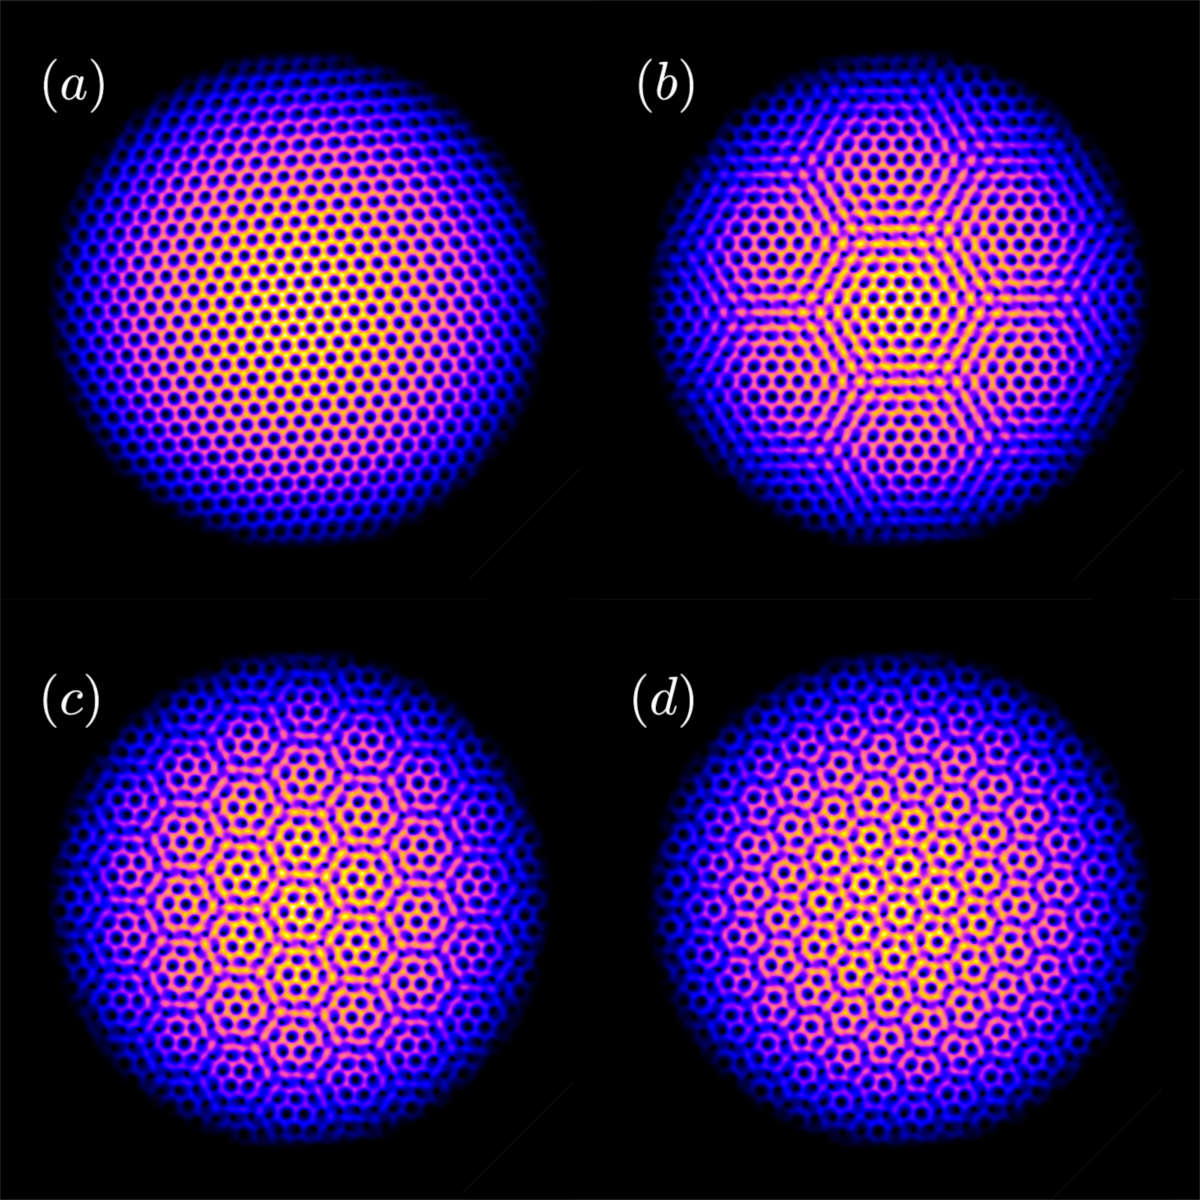
\includegraphics[width=0.48\textwidth]{ch4_kickit/fig4}
			\caption{Condensate density at $t=1.4\times10^{-2}$ s for several optical lattice rotation angles. The cell size of the super-lattice structures can be seen to shrink as the angle is increased. The angles for the examples shown are $(a)~\theta_\Delta=0$, $(b)~\theta_\Delta=2\pi/45$, $(c)~\theta_\Delta=4\pi/45$, $(d)~\theta_\Delta=2\pi/15$. }
			\label{fig:moire_density}
		\end{figure}

    However, if the angle between both lattices is finite, and not an integer multiple of $\pi/3$, superlattice structures appear after a short time (see Fig.~\ref{fig:moire_density}(b)-(d)), which have a structure cell size that decreases for increasing values of $\theta_\Delta\in[0,\pi/6]$ and beyond which increases for larger values until the misalignment angle reaches the lattice symmetry point again at $\theta_\Delta=\pi/3$. These structures are transient and several revivals can be observed before the condensate settles back into the vortex lattice structure with an increase in the background wave-number spread, as expected based on kicking the non-rotating condensate. An example of this for a fixed angle is shown in Fig.~\ref{fig:dtheta20_ev}.

	\begin{figure}[bt]
		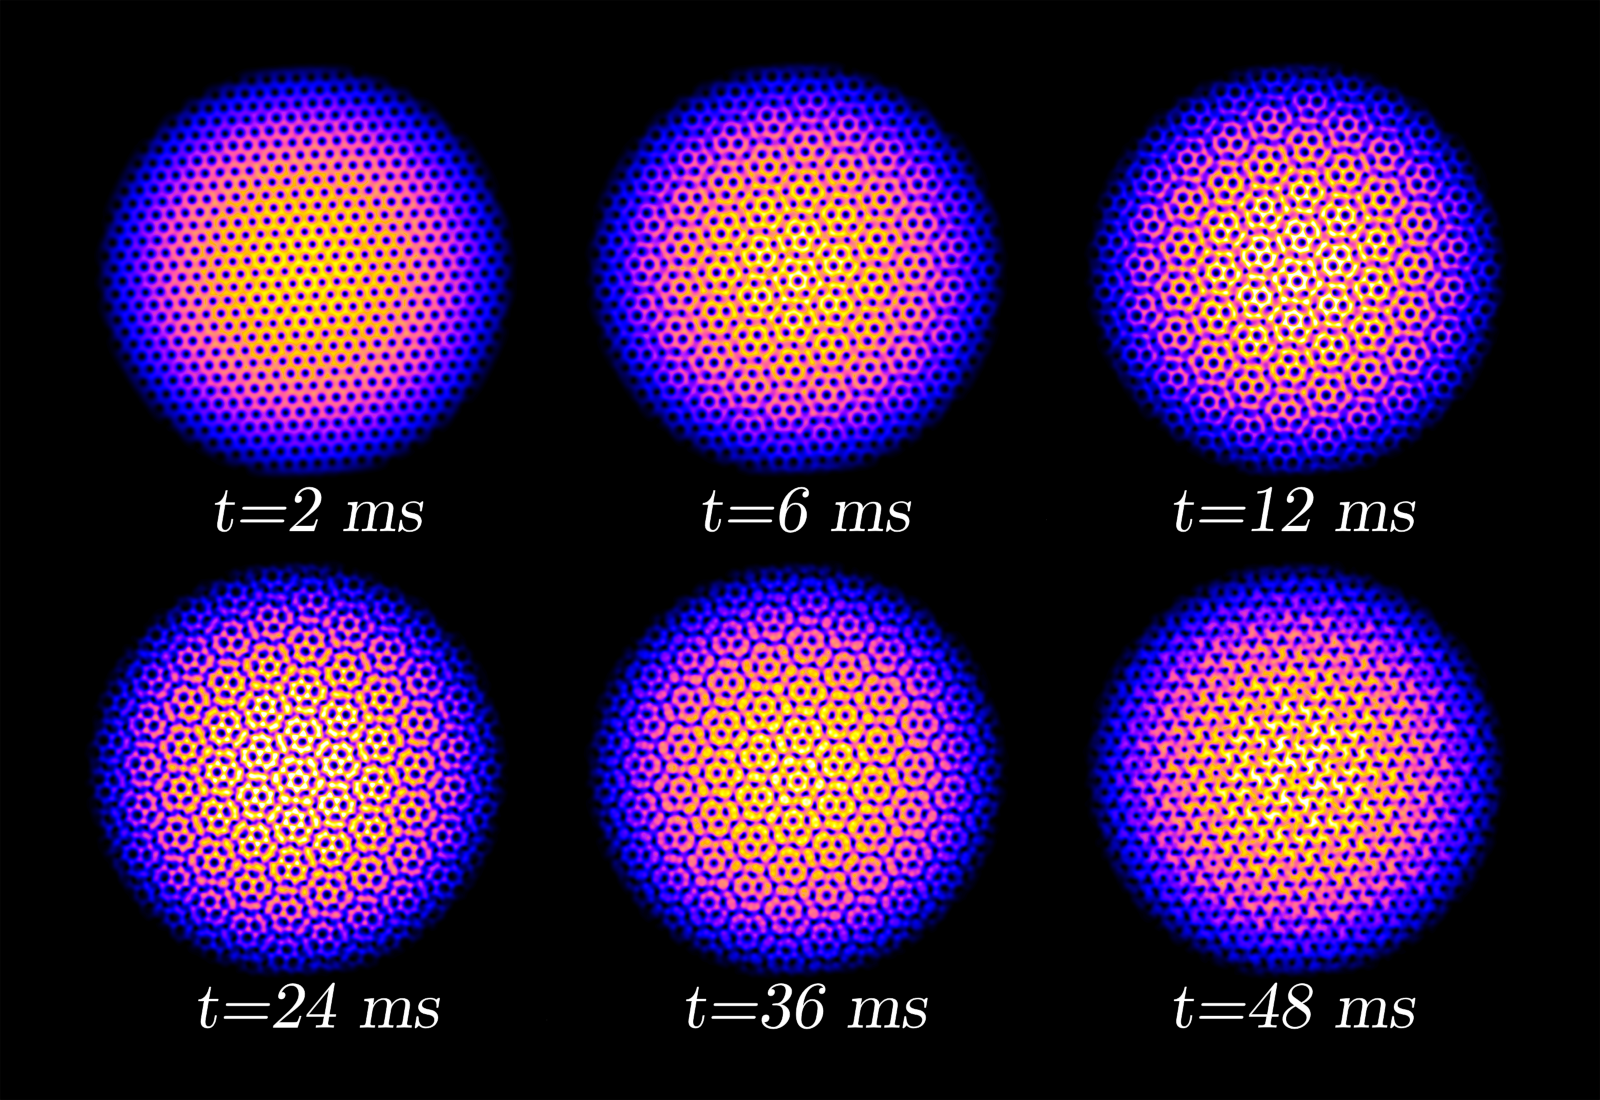
\includegraphics[width=0.48\textwidth]{ch4_kickit/fig5}
		\caption{Condensate density after receiving a kick with $\theta_\Delta=\pi/9$. The appearance and disappearance of a moir\'e structure with wavelength $\lambda_M \approx 2.9 a$ over a timescale of about $50$ ms can be seen.}
		\label{fig:dtheta20_ev}
	\end{figure}

    To explain the interference patterns observed for misaligning the optical and the vortex lattice, we employ moir\'e interference theory \cite{SS:Kerman_jphyscon_2012}. Moir\'e patterns are known to appear when two periodic structures are overlaid while slightly misaligned to each other and can be calculated from the reciprocal lattice vectors. In all generality, any choice of equidistantly separated reciprocal lattice vectors be parameterised as
    	\begin{equation}
    		\mathbf{g}_{l} = g_0 \left[ \sin\left( \frac{2\pi l}{\alpha}+\theta \right),\, \cos\left( \frac{2\pi l}{\alpha} +\theta\right) \right],
    	\end{equation}
    where $\alpha$ describes the rotational symmetry of the lattice, $l$ labels the vector direction on the unit circle, $\theta$ is the angle with respect to a chosen coordinate system and $g_0$ is the reciprocal lattice constant. For our commensurate and triangular lattices we have $g_0=4\pi/(\sqrt{3}a)$, $\alpha=6$ and the vector directions are $l=\left[0\dots\alpha-1\right]$. As only the relative mis-alignement between the vortex and the phonon lattice matters, we choose $\theta=0$ for the vortex lattice and $\theta=\theta_\Delta$ for the optical potential alignment.
    All possible wavelengths that can appear in an interference pattern between two such lattices in real space are then given by
    	\begin{equation}
    		\lambda_{ll'} = \frac{\lambda_0}{|\mathbf{\mathbf{g}_{ll'}|}},
    		\label{eq:InterferenceVectors}
    	\end{equation}
    where
    $\mathbf{g}_{ll'}=\mathbf{g}_{l}^{\text{V}}-\mathbf{g}_{l'}^{\text{P}}$, and
    $\lambda_0 = 4\pi/\sqrt{3}$ for the commensurate triangular lattices.
    One can see from Fig.~\ref{fig:dtheta20_ev} that a pattern matching the longest wavelength, $\lambda_M= \max[\lambda_{ll'}] \approx 2.9 a$, appears around $t=24$~ms and is clearly the most visible one. While patterns with shorter wavelength exist, they are harder to discern in our system and we therefore concentrate on the lowest wave-number in the following. It should be noted that given sufficient time the higher order wave-numbers do influence the dynamics, but the system remains dominated by the lowest wave-number. Due to coupling between adjacent modes in the system, all interference patterns tend to become hard to discern after some time. It is expected (but not investigated) that due to the Talbot effect (reference) in the long time limit the interference patterns will eventually reappear.

    In $\mathbf{k}$-space the shortest $|\mathbf{g}_{ll^\prime}|$ corresponds to adjacent wave-vectors with the smallest $\theta_\Delta$ between them (see inset in Fig.~\ref{fig:moire_lambda_1}). Due to the symmetry of the lattices the most visible structures are therefore given by $\lambda_M=\lambda_{00}$ for $\theta_\Delta\in[0,\pi/6]$ and $\lambda_M=\lambda_{01}$ for $\theta_\Delta\in[\pi/6,\pi/3]$ (see inset of Fig.~\ref{fig:moire_lambda_1}).
    While this symmetry assumption no longer holds strictly true after the system has been kicked, it is still fulfilled to a very good approximation during the initial dynamics. One can then obtain the wavelength of the dominating moir\'e structure as~\cite{jns-moire,nphys2272}
    		\begin{equation}
    		\lambda_M = \frac{a}{2\sin(\eta/2)},
    		\label{eqn:moire_size}
    	\end{equation}
    where $\eta=\min\{\theta_\Delta,\frac{\pi}{3} - \theta_\Delta \} $  (see Fig.~\ref{fig:moire_lambda_1}).
These super-structures become observable when the wavelength becomes smaller than the radius of the condensate, which for the chosen parameters is $\lambda_M \approx 11a$ and which corresponds to an angle $\theta_\Delta \approx \pi/36$.
One can see from Fig.~\ref{fig:moire_lambda_1} that once the relative angle is increased beyond this value
the structure sizes shrink to a minimum value at the point of complete misalignment, $\theta_\Delta=\pi/6$, giving $\lambda_M\approx 1.93\,a$, and increase again up to the point of symmetry. Beyond this point the whole behaviour starts over, due to the symmetry of the lattice. Note that in principle the above procedure can be carried out for square or other optical lattice geometries.

\begin{figure}[tb]
	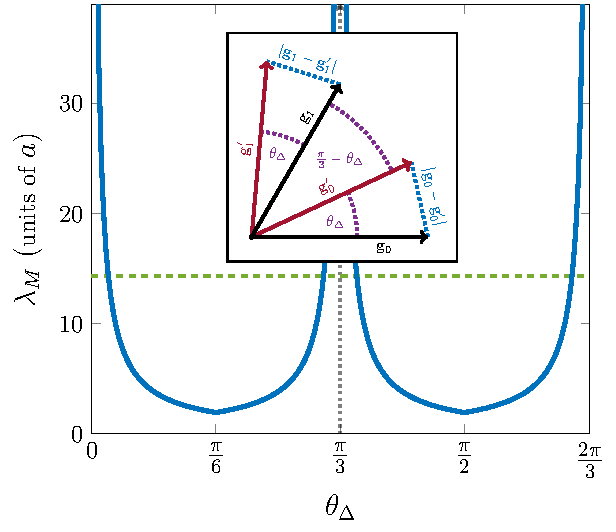
\includegraphics[width=0.48\textwidth]{ch4_kickit/fig6}
	\caption{Size of the resulting moir\'e super-structures as a function of the relative angle between the vortex and optical lattice. The dashed green line indicates the condensate radius. Inset: The different vectors in $\mathbf{k}$-space of the two lattices, with the optical lattice rotated by an angle $\theta_\Delta$. The $\mathbf{g}_{ll'} = |\mathbf{g}_l - \mathbf{g}_l'|$ vectors defining the dominant moir\'e wavelength are those for which the enclosed angle is smallest. }
	\label{fig:moire_lambda_1}
\end{figure}

    The appearance of the moir\'e vector in $k$-space can be confirmed from the numerical simulations by looking at the compressible kinetic energy spectra which we display in Fig.~\ref{fig:dtheta_kspec}. Apart from the dominant peaks corresponding to the underlying triangular geometry of the Abrikosov lattice, which are independent of $\theta_\Delta$ (straight lines in Fig.~\ref{fig:dtheta_kspec}), a number of additional peaks appear. Their position is a function of the misalignment angle and the lowest wave-number that appears increases its value with increasing $\Delta_\theta$. This is consistent with the moir\'e model and the appearance of density structures of differing size.

    Furthermore, a symmetric repeat of this structure about the $\theta_\Delta=\pi/6$ point is also visible, which corresponds to the $\pi/3 - \theta_\Delta$ lattice vector component. The minimum wavelength observed agrees with the theoretically determined minimum value of $\lambda_M\approx 1.93\,a$ and all other values over the range of observed angles. Note that for the higher harmonics at larger wave-numbers similar behaviour exists and is also covered by the moir\'e model.
	\begin{figure}[tb]
		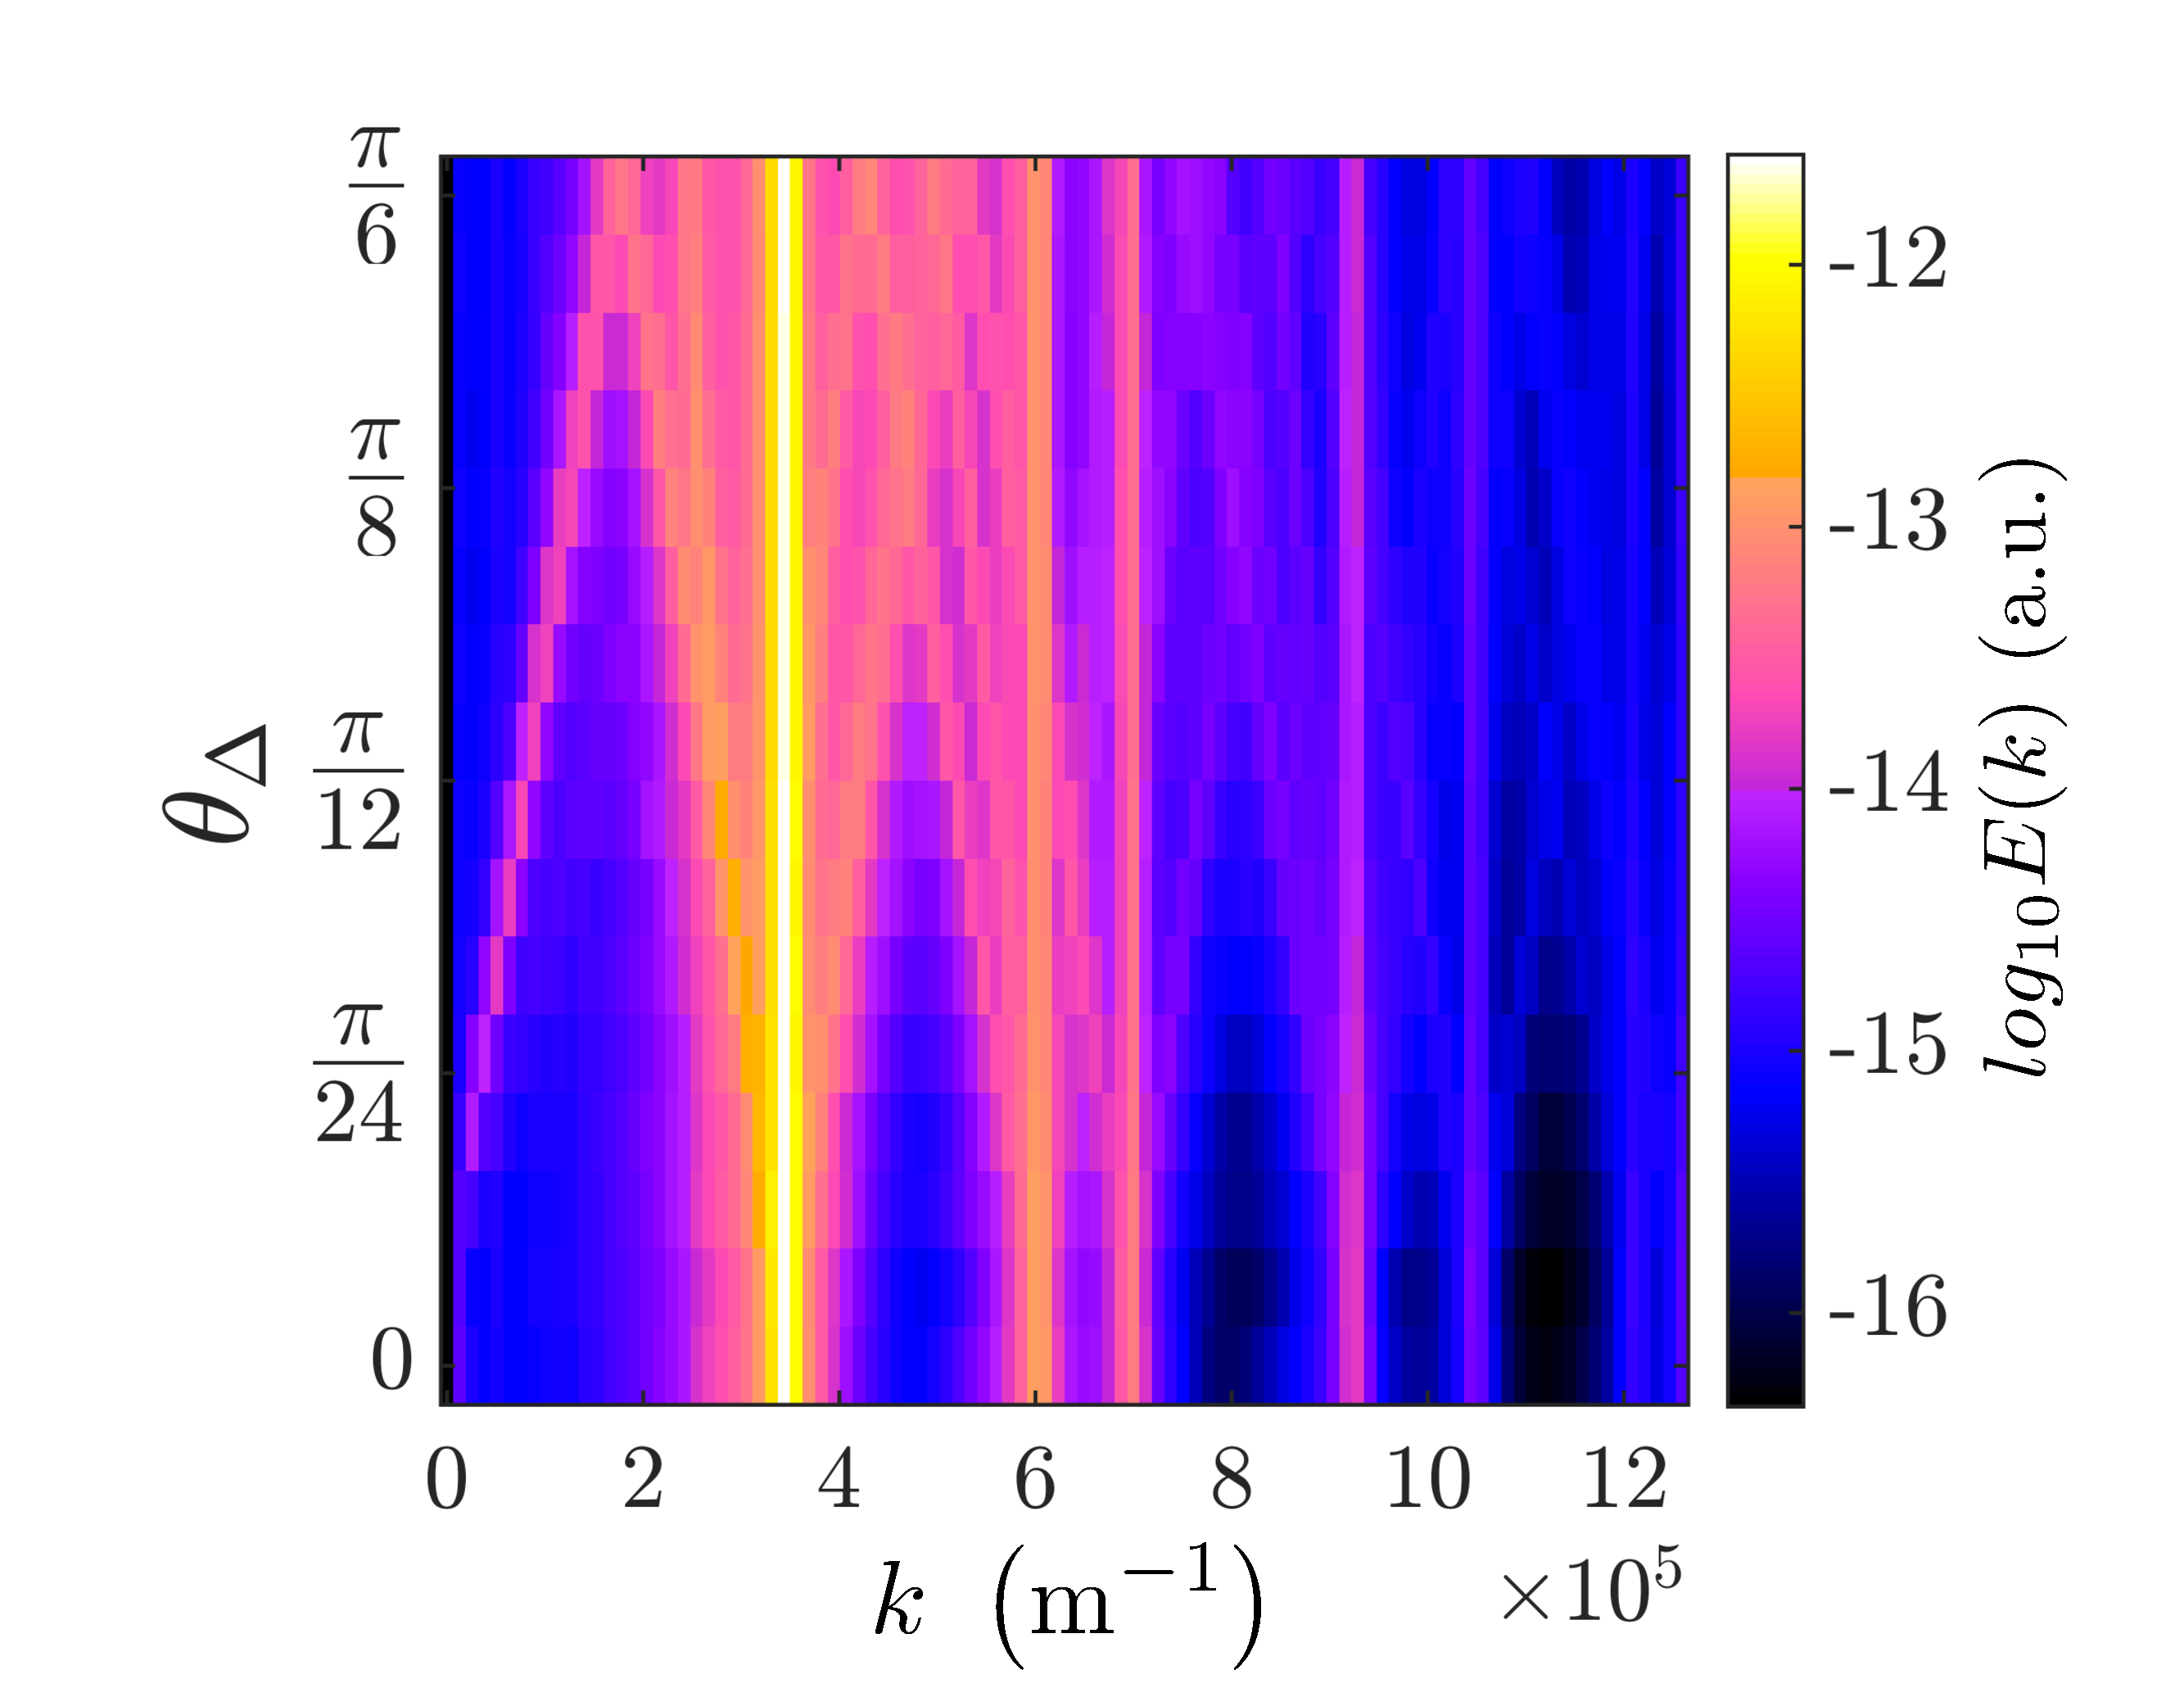
\includegraphics[width=0.48\textwidth]{ch4_kickit/fig7}
		\caption{Compressible kinetic energy spectrum as a function of $\theta_\Delta$. All values are time-averaged over an interval $t=0$ s to $t=1$ s. The moir\'e peak corresponding to the lowest wave-number can be seen shifting to larger values for increasing angles and similar behavior is visible for the higher order components.}
		\label{fig:dtheta_kspec}
	\end{figure}

    I will now briefly discuss what happens for stronger kicking, or when the two lattices are non-commensurate. In the above the strength of the kicking pulse was chosen such that its perturbation only leads to a phase imprinting \cite{Vtx:Dobrek_pra_1999,BEC:Denschlag_science_2000}, with minimal change to the initial density. If one increases the kicking intensity the situation becomes quite different and one can see from Fig.~\ref{fig:kickp20k}(a) that higher order wave-numbers become more strongly excited. This, in turn, leads to modulations of the condensate density at shorter wavelength and an example is shown in Figs.~\ref{fig:kickp20k}(b)-(e). However, as for fully realistic experimental situations it is necessary to consider the heating of the condensates due to the disturbance once the kicking becomes stronger, we restrict this investigation to low intensity pulses.

\begin{figure}[tb]
	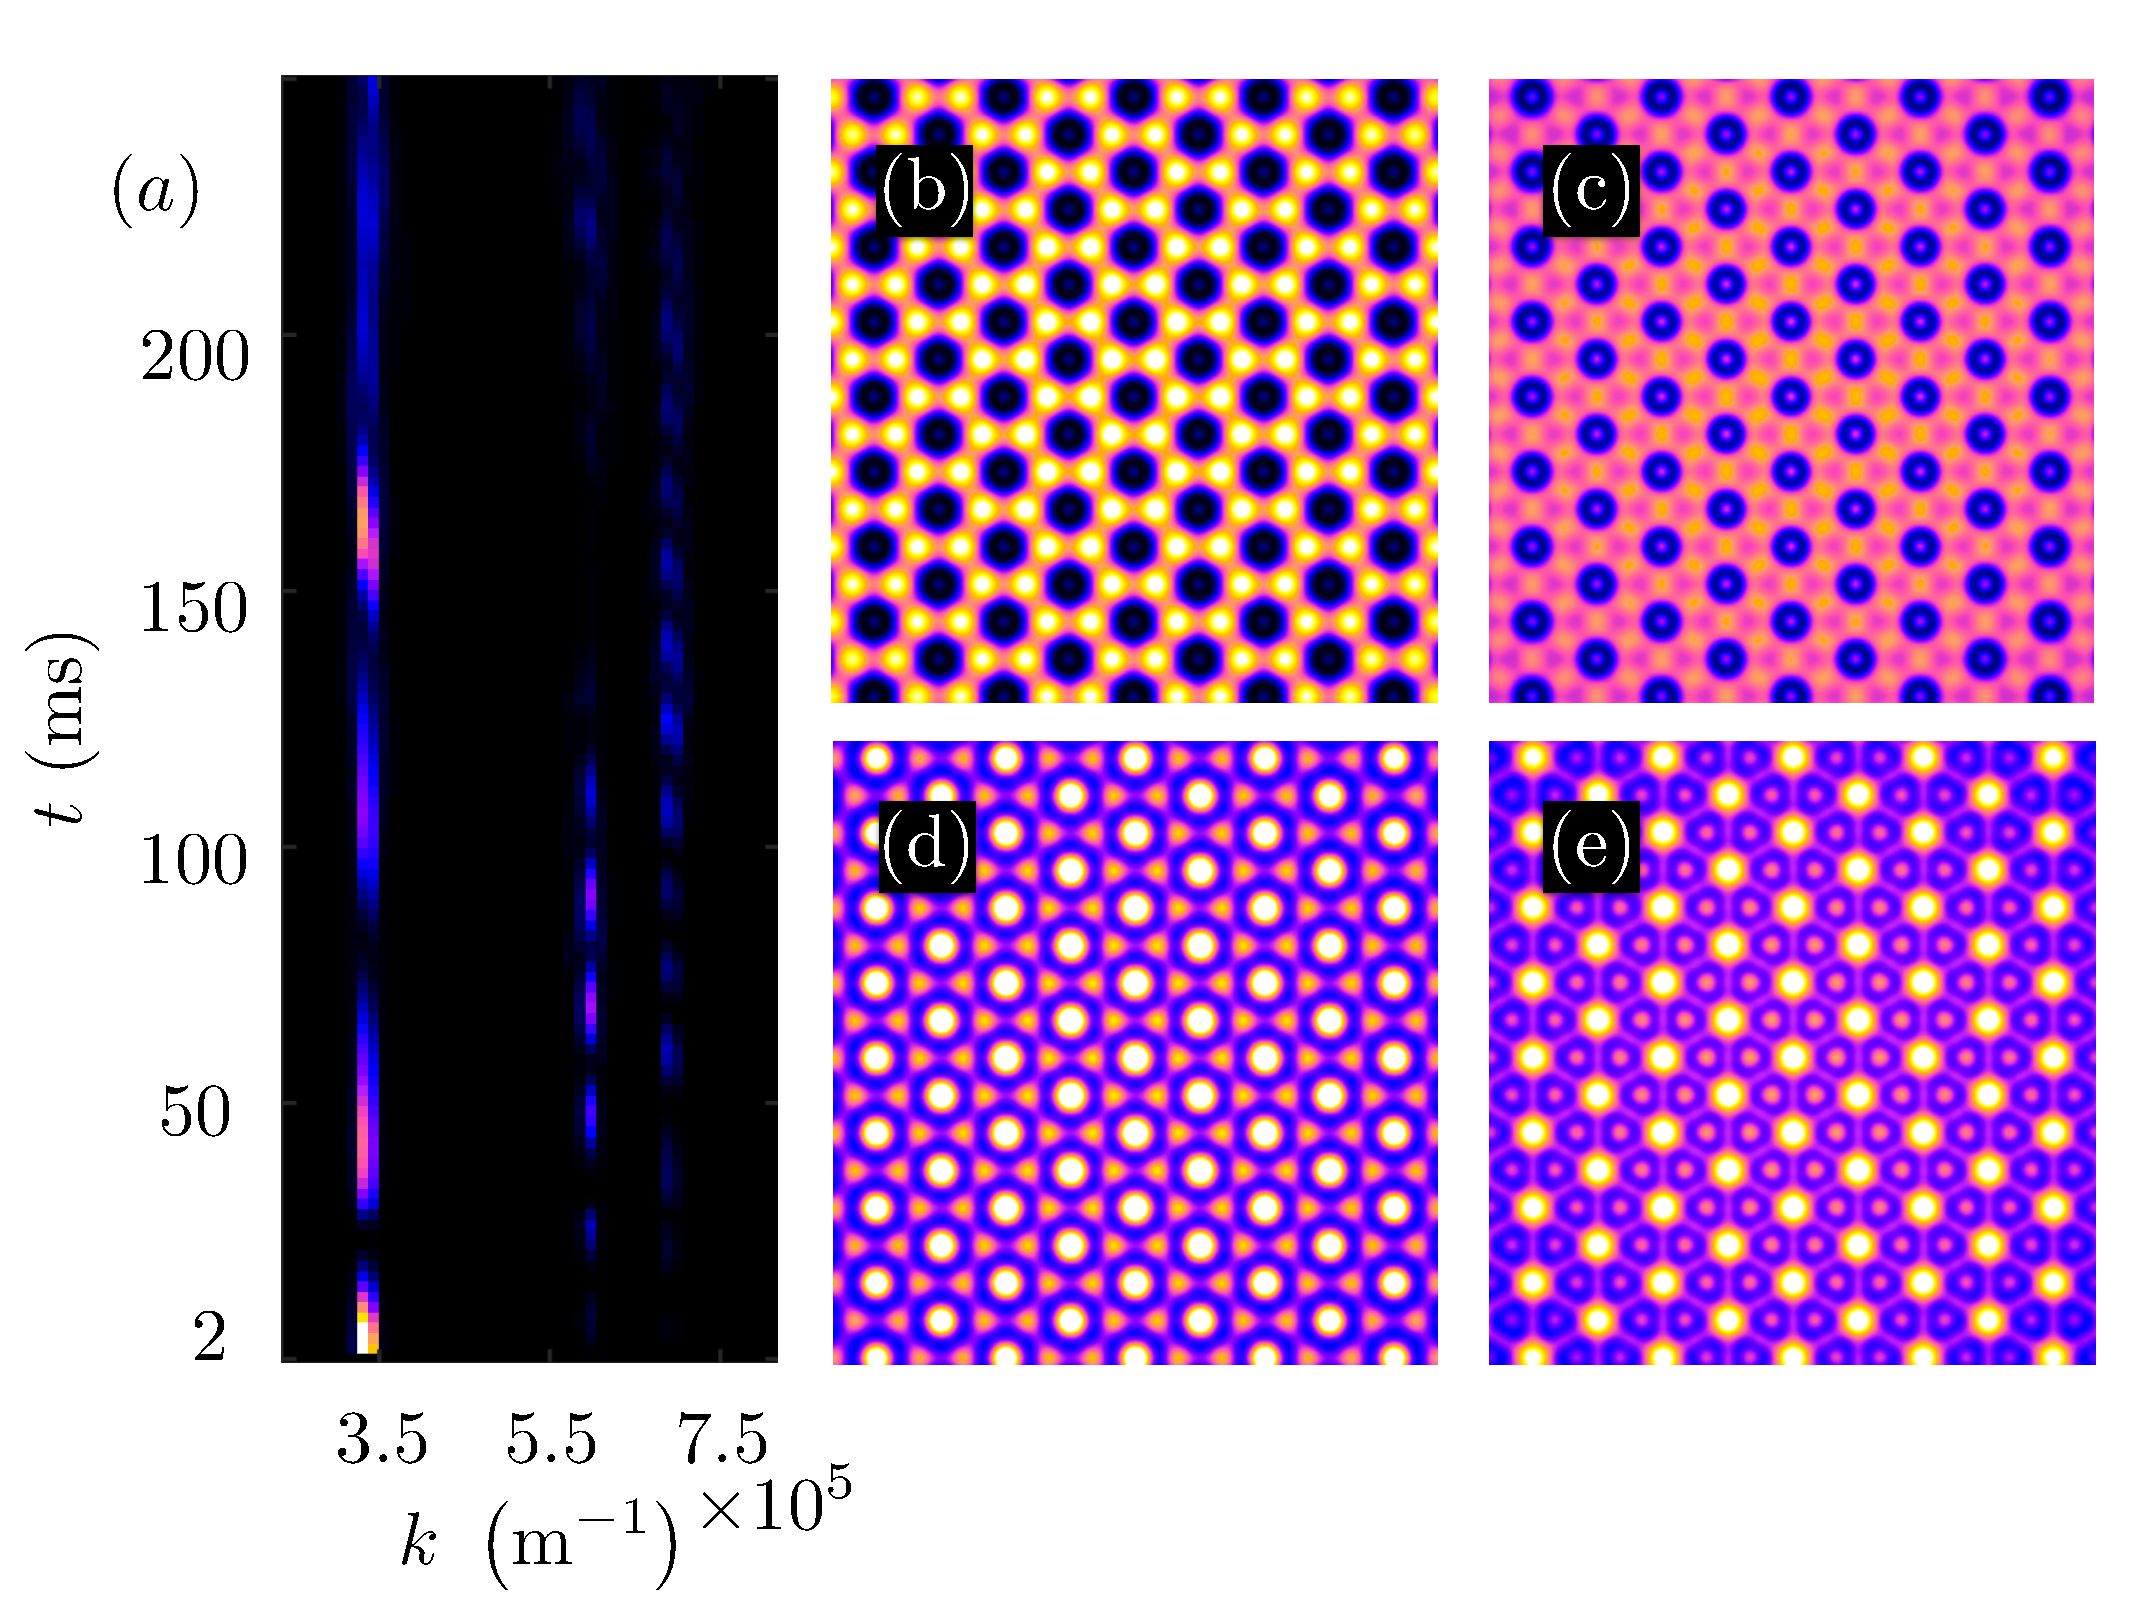
\includegraphics[width=0.48\textwidth]{ch4_kickit/fig8}
	\caption{(a) For a kicking strength of $V_0 = 5.4\times10^{-2}\mu$ for a non-rotating condensate higher order modes become non-negligible contributions to the compressible kinetic energy spectrum. This leads to a variety of different density structures, with some close-ups shown for (b) 24 ms, (c) 36 ms, (d) 56 ms, and (e) 88 ms. Note that the larger structures in these plots are given by the optical lattice constant, which sets the scale.}
	\label{fig:kickp20k}
\end{figure}

    A situation where the optical and the vortex lattice have different lattice constants can be imagined to appear naturally due to experimental uncertainties. Defining $a_o = a_v(1+\epsilon)$ the expression in eq.~\eqref{eq:InterferenceVectors} can be calculated to be
    \begin{equation}
    	\lambda_M = \frac{a_v(1+\epsilon)}{\sqrt{2(1+\epsilon)(1-\cos\theta) + \epsilon^2}}
    	\label{eqn:moire_size_eps}
    \end{equation}
    which reduces to eq.~\eqref{eqn:moire_size} for $\epsilon=0$. Evaluating this expression shows that the largest moir\'e wavelength changes slightly for small values of $\epsilon$, but it remains distinct enough from the underlying wave-vectors to stay visible in the evolution. This ensures that the system examined here is experimentally realistic.

\subsection{Conclusions}
\label{subs:ch4_conc}
Will originally the intent of the proposed system was to investigate chaotic dynamics, it was instructive to investigate the interference pattern resulting from the kicking. As observed in the incompressible spectrum, kicking gave negligible effect to the vortex positions, with the lattice remaining well defined with strongly defined spacings, even in the long time limit. The optical lattice kicks did little to dislodge the vortices, and solely modified the background density around the cores. One could observe that the vortex lattice remains incredibly stable and strongly resilient to perturbations and modulations in density.

While not as was intiailly expected, this interference effect had some nice consequences. As a tool to test the periodidicity of a structure that is too small to resolve without time of light, the moir\'e super-lattice structure may be useful for just that. Carrying out preliminary work in zig-zag and linear crystals in conjunction with A. Barahmi and Th. Busch, it was observed that without well defined periodic behaviour there is negligible observation of any peaks in the compressible energy spectrum. As such, there was negligible discernable pattern in density. It is expected that for such an effect to be useful in highly periodic systems, with well defined wave-vectors. It remains an open question as to whther this can be used in a realistic experimental apparatus.


%\section{Kinetic energy decomposition}

%\section{Superlattice structures}

%\section{Moir\`e interference theory}

\fi
%%%%%%%%%%%%%%%%%%%%%%%%%%%%%%%%%%%%%%
\newif\ifdefect
\ifdefect
    \chapter{Defect engineering}
        %%%%%%%%%%%%%%%%%%%PAPER
%%%%%%%%%%%%%%%%%%%%%%%%%%%%%%%%%%%%%%%%%%%%%%%%%%%%%%%%%%%%%%%%%%%%%%%%%%%%%%%%%%%%%%%%%%%%%%%%%%%%%%%%%%%%%%%%%%%%%%%%%%%%%%%%%%%%%%%%%%%%%
\subsection{Rapidly rotating BEC}
%%%%%%%%%%%%%%%%%%%%%%%%%%%%%%%%%%%%%%%%%%%%%%%%%%%%%%%%%%%%%%%%%%%%%%%%%%%%%%%%%%%%%%%%%%%%%%%%%%%%%%%%%%%%%%%%%%%%%%%%%%%%%%%%%%%%%%%%%%%%%
For this work, we numerically solve the Gross-Pitaevskii equation in two dimensions, assuming a strong confinement along the third axis.
This allows all dynamics to be restricted to the $xy$ plane, with vortices behaving as charged particles in a neutral background. In the
frame corotating with the condensate, this can be modeled as
\begin{equation}
	 i\hbar\partial_t \Psi\left(\mathbf{x},t\right) = \left[ -\frac{\hbar^2}{2m}\nabla^2 + V\left(\mathbf{x}\right) + g\vert \Psi\left(\mathbf{x},t\right) \vert^2 - \Omega L_z \right]\Psi\left(\mathbf{x},t\right)
\end{equation}
where $V\left(\mathbf{x}\right)$ is the trapping geometry, $\Omega$ is the trap rotation frequency, and $L_z$ is the angular momentum
operator along the $z$-direction. For the rapidly rotating case, the vortices form an ordered triangular lattice, that rotates equivalently
to a solid-body in the large number limit. Deviations from the solid-body rotation can be seen for trajectories in the limit of long times
(~10 s). This is very likely due to long-wavelength Tkachenko modes in the condensate, and following the analysis of [Baym, Tk modes of vtx latt in rr BEC]
has a frequency much longer than the lifetime of the system for our given rotation rate.
%However, due to the density inhomogeneities of a harmonically trapped condensate, and the likelihood of shearing this is (I think) expected.
The lattice is well ordered and behaved at timescales on the order of upto few seconds, as well as away from the condensate edges, and so we
will restrict our analysis therein.

As condensates are highly controllable in the lab (cite many papers), we consider the use of many common experimental techniques to engineer
specific states otherwise difficult in solid-state materials. One such set of systems are those of crystals with controllable defects, which
although (relatively) easily created classically (cite bead packing, etc), are difficult experimentally in quantum systems due to the sizes
of interatomic spacings. Here we propose the use of phase-imprinting (cite) as a means of achieving such defects in a Bose-Einstein
condensate. Through direct manipulation of the condensate phase, vortices may be added or removed from specific locations in the system.

%%%%%%%%%%%%%%%%%%%%%%%%%%%%%%%%%%%%%%%%%%%%%%%%%%%%%%%%%%%%%%%%%%%%%%%%%%%%%%%%%%%%%%%%%%%%%%%%%%%%%%%%%%%%%%%%%%%%%%%%%%%%%%%%%%%%%%%%%%%%%
\subsection{Order/disorder}
%%%%%%%%%%%%%%%%%%%%%%%%%%%%%%%%%%%%%%%%%%%%%%%%%%%%%%%%%%%%%%%%%%%%%%%%%%%%%%%%%%%%%%%%%%%%%%%%%%%%%%%%%%%%%%%%%%%%%%%%%%%%%%%%%%%%%%%%%%%%%
Given the localised defect disturbs the lattice after sufficiently long times, we can examine if the lattice moves from global ordered to
disordered following the addition or removal of another site over the course of time. For a two-dimensional material, KTHNY theory describes
the transitions from a solid crystalline to amorphous fluid phase, via an intermediate hexatic phase. This state is generally characterised
by the translational and orientational correlation functions long-ranged behaviour. As we have an inhomogeneous density profile, and thus
lattice outside a given radius, the use of translational correlations does not make much sense. Orientational correlations however, which
measure how the lattice aligns to a particular angle, should suffice when combined with the density structure factor,
$S = \int d\mathbf{r}e^{i\mathbf{k}\cdot\mathbf{r}}|\Psi|^2$. True crystaline behaviour is given by orientational constant values, with
power-law decay is expected for a hexatic phase, and exponential decay for an amorphous fluid (neglecting translational correlations).

%%%%%%%%%%%%%%%%%%%%%%%%%%%%%%%%%%%%%%%%%%%%%%%%%%%%%%%%%%%%%%%%%%%%%%%%%%%%%%%%%%%%%%%%%%%%%%%%%%%%%%%%%%%%%%%%%%%%%%%%%%%%%%%%%%%%%%%%%%%%%
\subsection{Phase imprinting defects}
%%%%%%%%%%%%%%%%%%%%%%%%%%%%%%%%%%%%%%%%%%%%%%%%%%%%%%%%%%%%%%%%%%%%%%%%%%%%%%%%%%%%%%%%%%%%%%%%%%%%%%%%%%%%%%%%%%%%%%%%%%%%%%%%%%%%%%%%%%%%%
Phase imprinting has been shown as an effective tool for the creation of vortices within a Bose-Einstein condensate (cite). The signature of
a quantum vortex is given by a phase singularity, around which the phase winds through $\pm 2\pi$, depending upon the direct of rotation.
Through the use of the phase imprinting method, we can eliminate a vortex from the lattice by applying the correct phase profile. To
eliminate a vortex from the lattice we need only to apply the opposite phase winding to that of the vortex to be eliminated. The
instantaneous application of a phase singularity to the condensate will create phonon modes in the density, as will the annihilation event.
Since the induced phonons have been shown to yield minimal impact on the vortex lattice structure <ref my paper>, we can safely
ignore their contribution. The removal of a vortex from the lattice introduces a vacancy to the system.


We model the vortex lattice as a graph, where each vortex represents a node, and edges are given by nearest neighbours at most separated by
a distance $a_0$, for a triangular lattice configuration, or $\sqrt{2}a_0$ for a square lattice (see Fig. \ref{fig:vtxdist}). The inclusion
of the square lattice distance is chosen so that upon removal, the vortices can reconfigure their arrangement locally, and may move from
triangular to square geometries. As they behave like Coulombic particles with a profile that falls off as $r^{-1}$ we can consider that any
interactions outside these distances to be negligible.

\subsubsection{Lattice vacancy}
%%%%%%%%%%%%%%%%%%%%%%%%%%%%%%%%%%%%%%%%%%%%%%%%%%%%%%%%%%%%%%%%%%%%%%%%%%%%%%%%%%%%%%%%%%%%%%%%%%%%%%%%%%%%%%%%%%%%%%%%%%%%%%%%%%%%%%%%%%%%%
The removal of a vortex from the vortex is thus expected to affect only the nearest neighbours by altering their velocity well, with the
overall angular momentum of the condensate decremented by a single quantum. The resulting vacancy, following a vortex removal, remains
localised to its respective position within the lattice for long times, regardless of initial placement (assuming not at edge)
(see Fig. \ref{fig:trajectory}). The
resulting stability of the nearest neighbours follows a decay of the honeycomb-like structure akin to that described by [statistical
topology of perturbed two-dimensional lattices]. Given enough time, this structure decays via one of the three possible means, creating a
locally disordered region with a grain boundary/disclination/dislocation? evident of the lattice change. However, even for long times, the
overall vortex lattice remains well structured, as evidenced by examining correlation functions of the vortex positions for both two-body,
and orientational correlations.


\iffalse
\include{g6rimg}
\fi

After the vortex removal, the system remains in a stable configuration, for a period on the order of 100+ ms (see Fig. \ref{fig:voronoi_area},
\ref{fig:voronoi_100ms}), after which the vortices begin to deviate from their lattice positions and attempt to fill the vacancy and balance
the inter-vortex forces.
\iffalse
\begin{figure}[tb]
	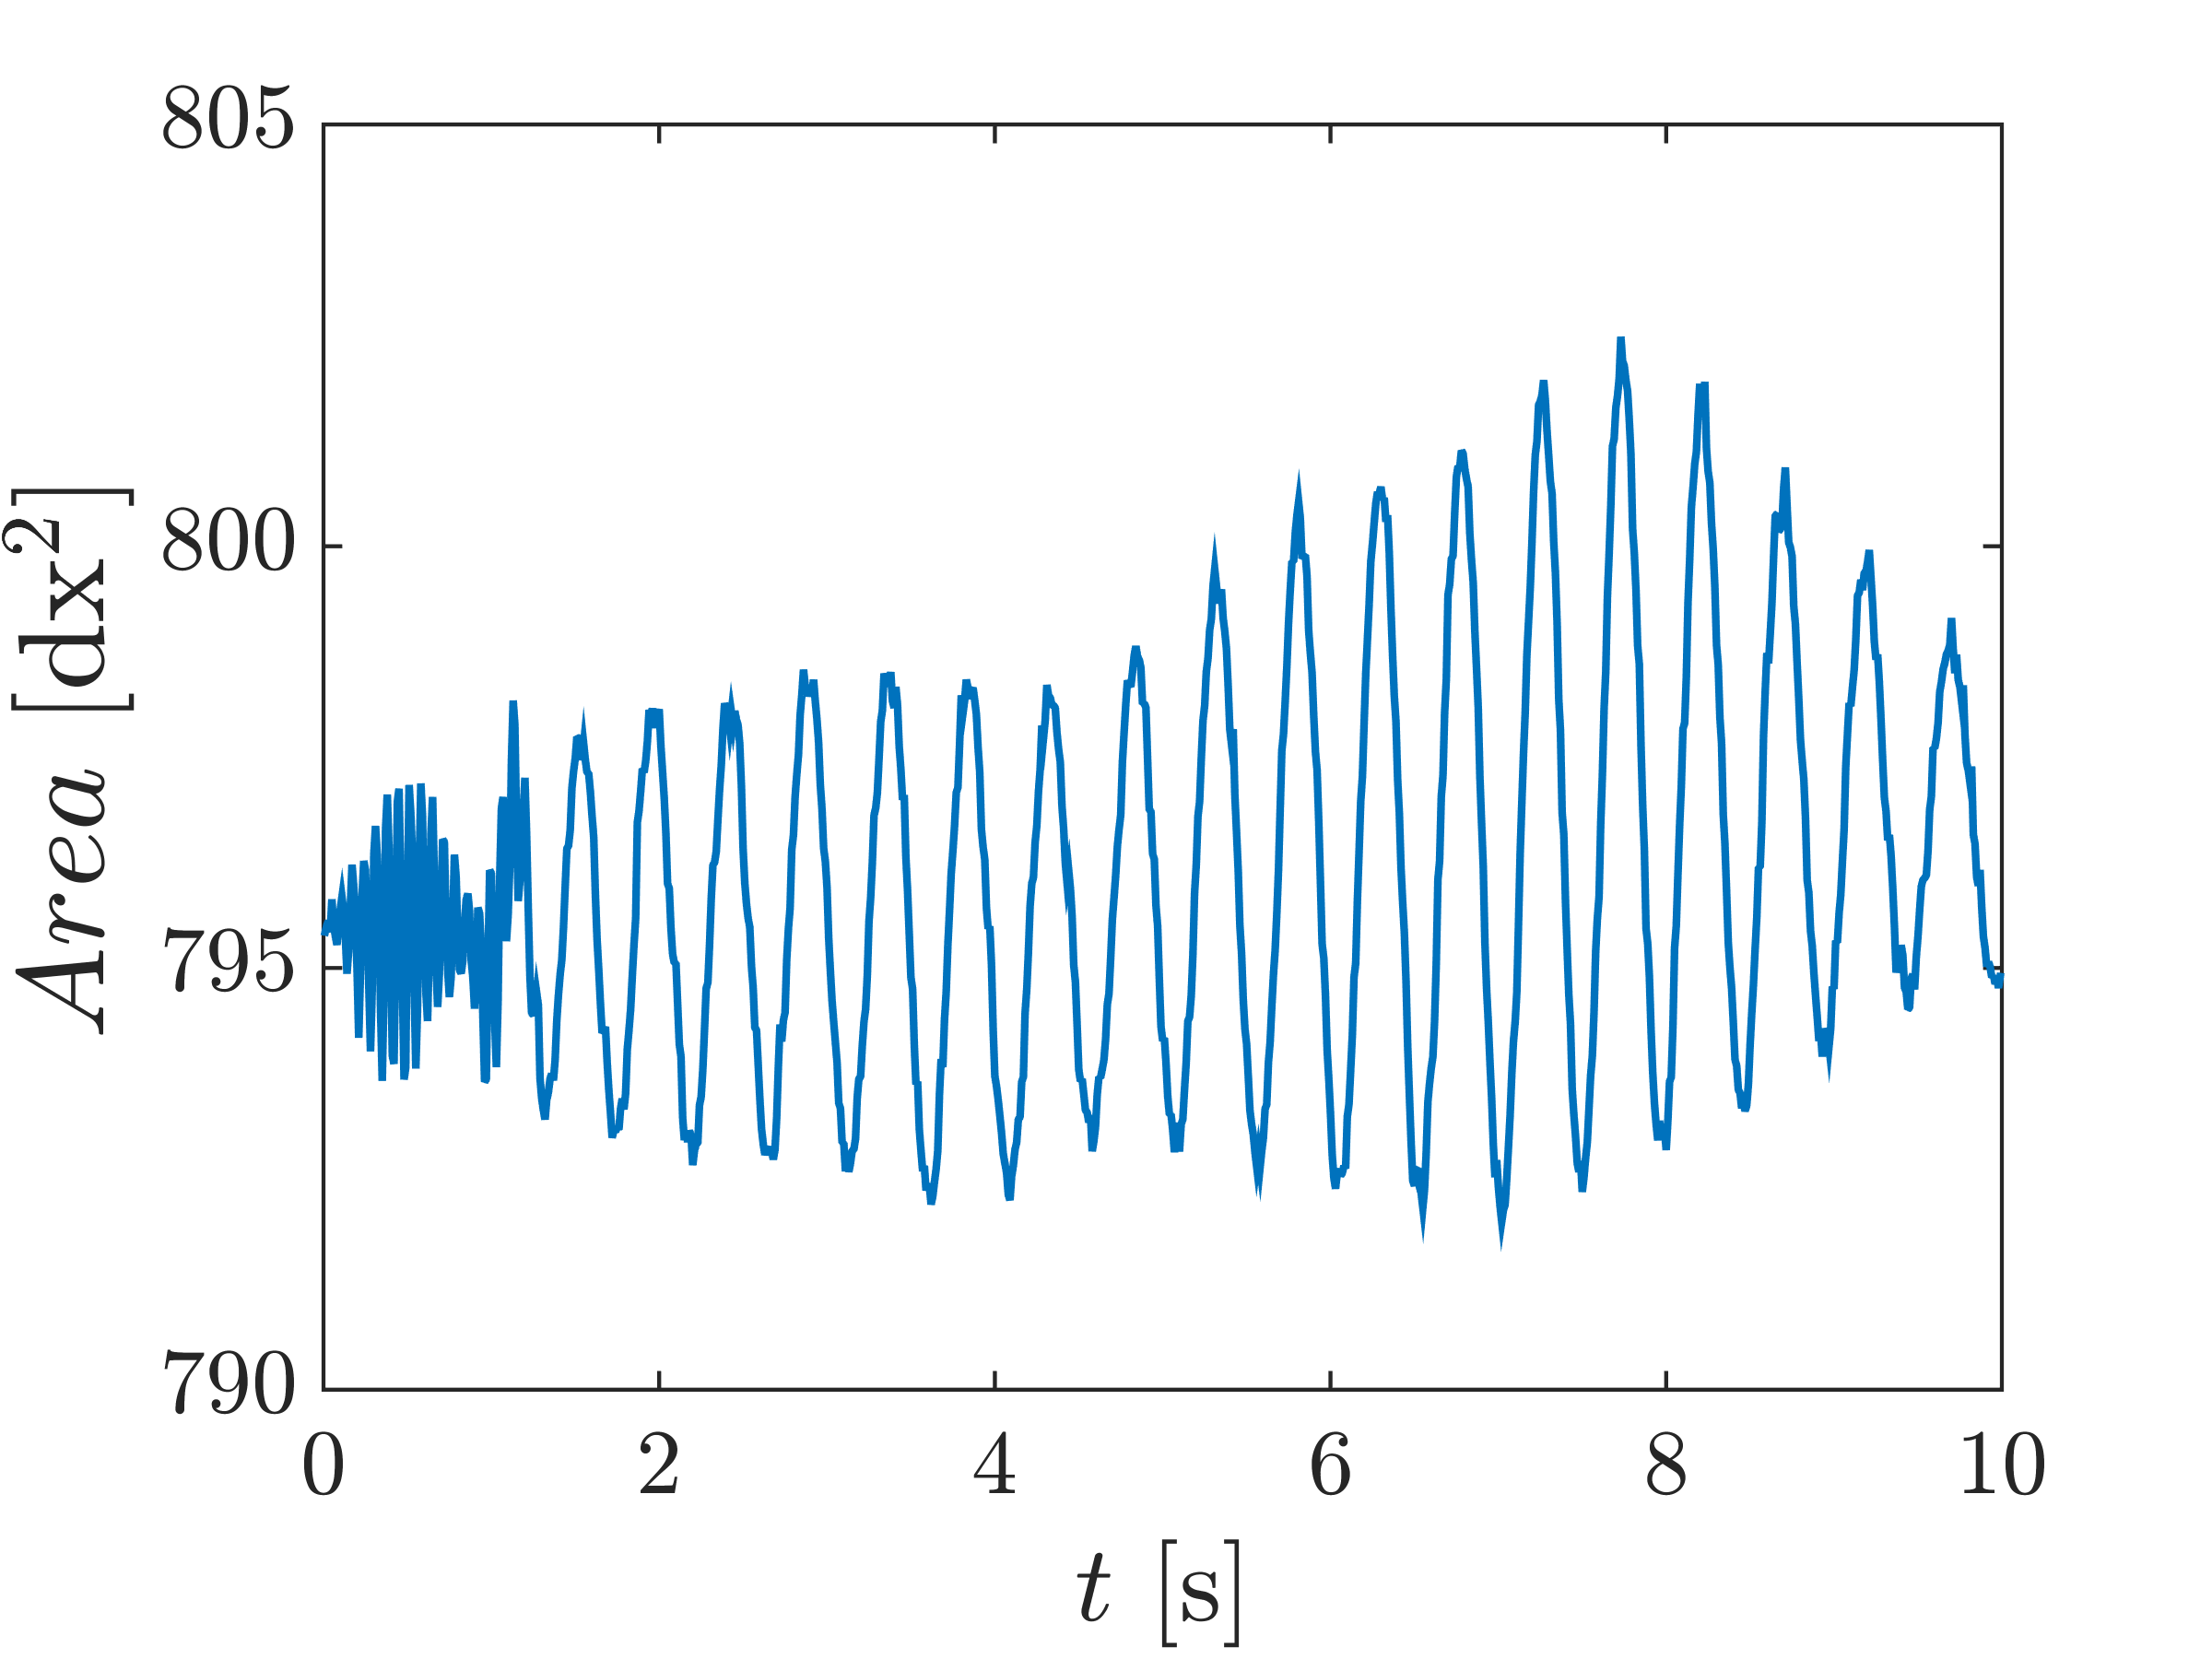
\includegraphics[width=0.48\textwidth]{imgs/Disloc_-1_centre_avgarea}
	\caption{Voronoi cell average area after removing vortex at condensate centre. }
	\label{fig:voronoi_area}
\end{figure}
\fi
Removing vortices at different positions in the lattice shows similar behaviour, with the effect on the velocity profile and trajectories of
other vortices being mostly localised around the removal site.

\iffalse
\begin{figure}[tb]
	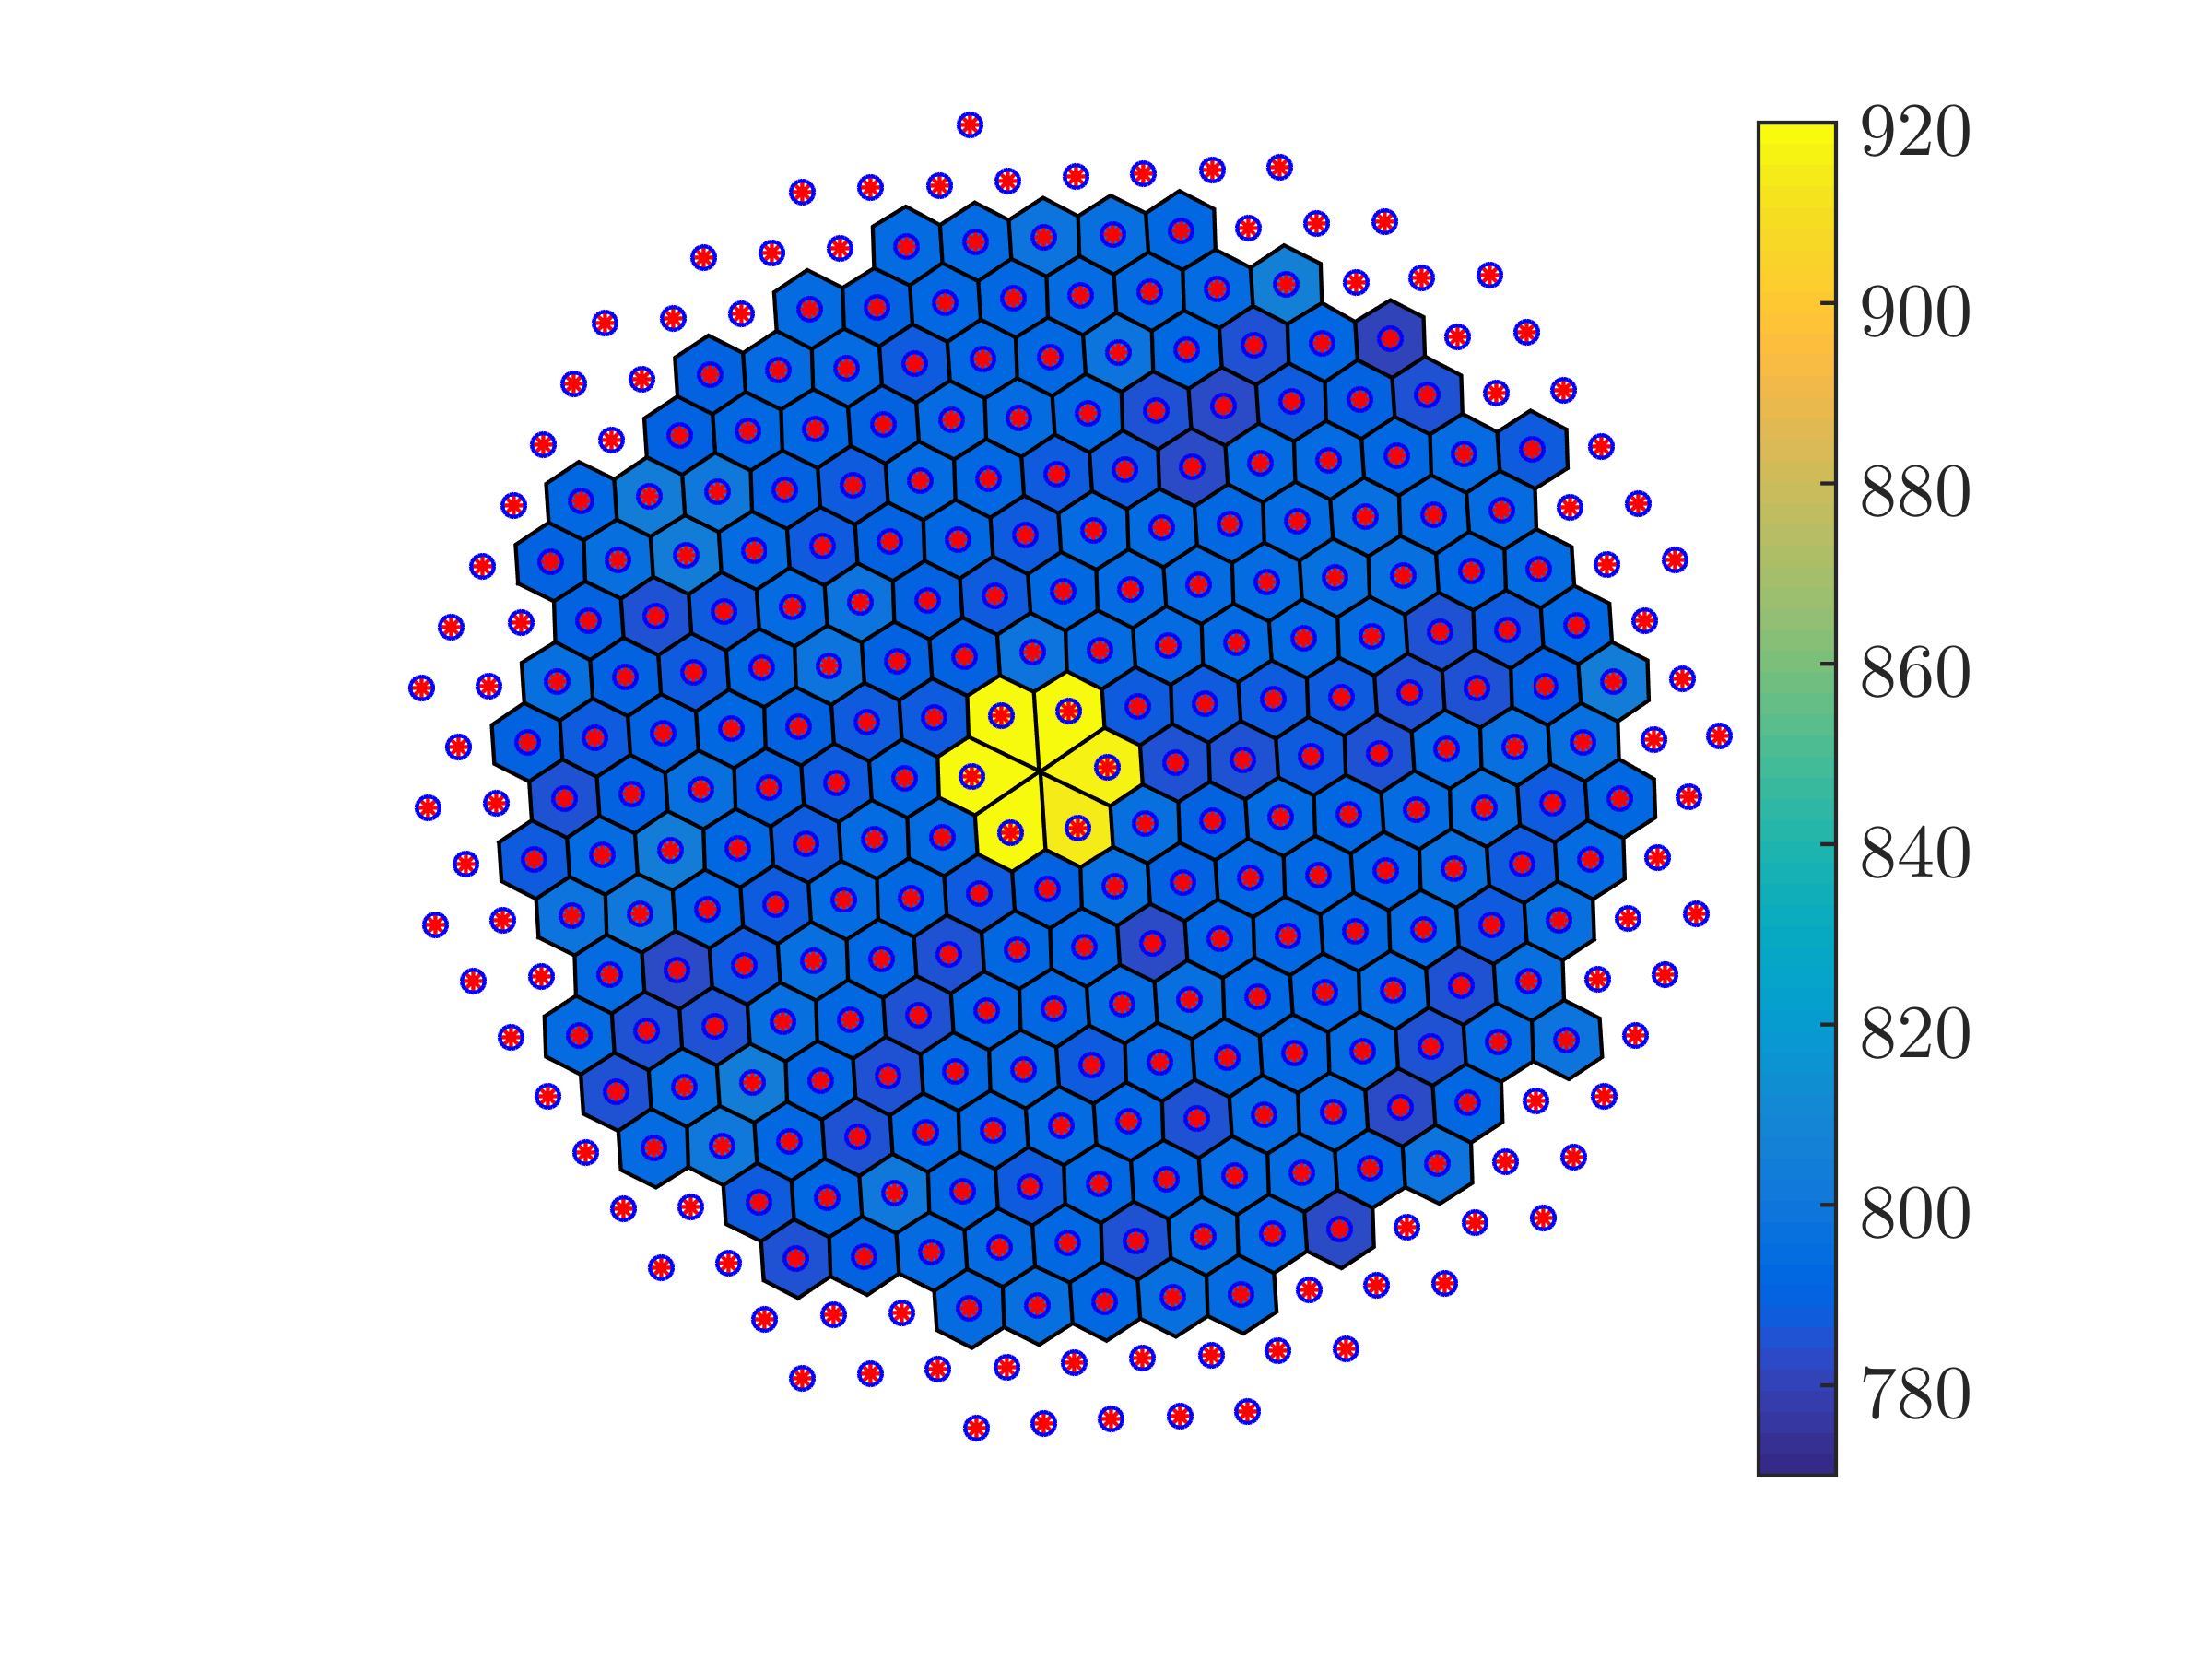
\includegraphics[width=0.48\textwidth]{imgs/Disloc_-1_centre_voronoi_t100ms_cbar}
	\caption{Voronoi cells after removing vortex at condensate centre for t=100 ms. Vortices at edge boundary neglected. }
	\label{fig:voronoi_100ms}
\end{figure}
\fi
Tracking the vortex distances traveled for different removal locations, and for a different number of removed vortices shows how much we
disturb the underlying lattice (see \ref{fig:vtxdist}).

\iffalse
\begin{figure}[tb]
	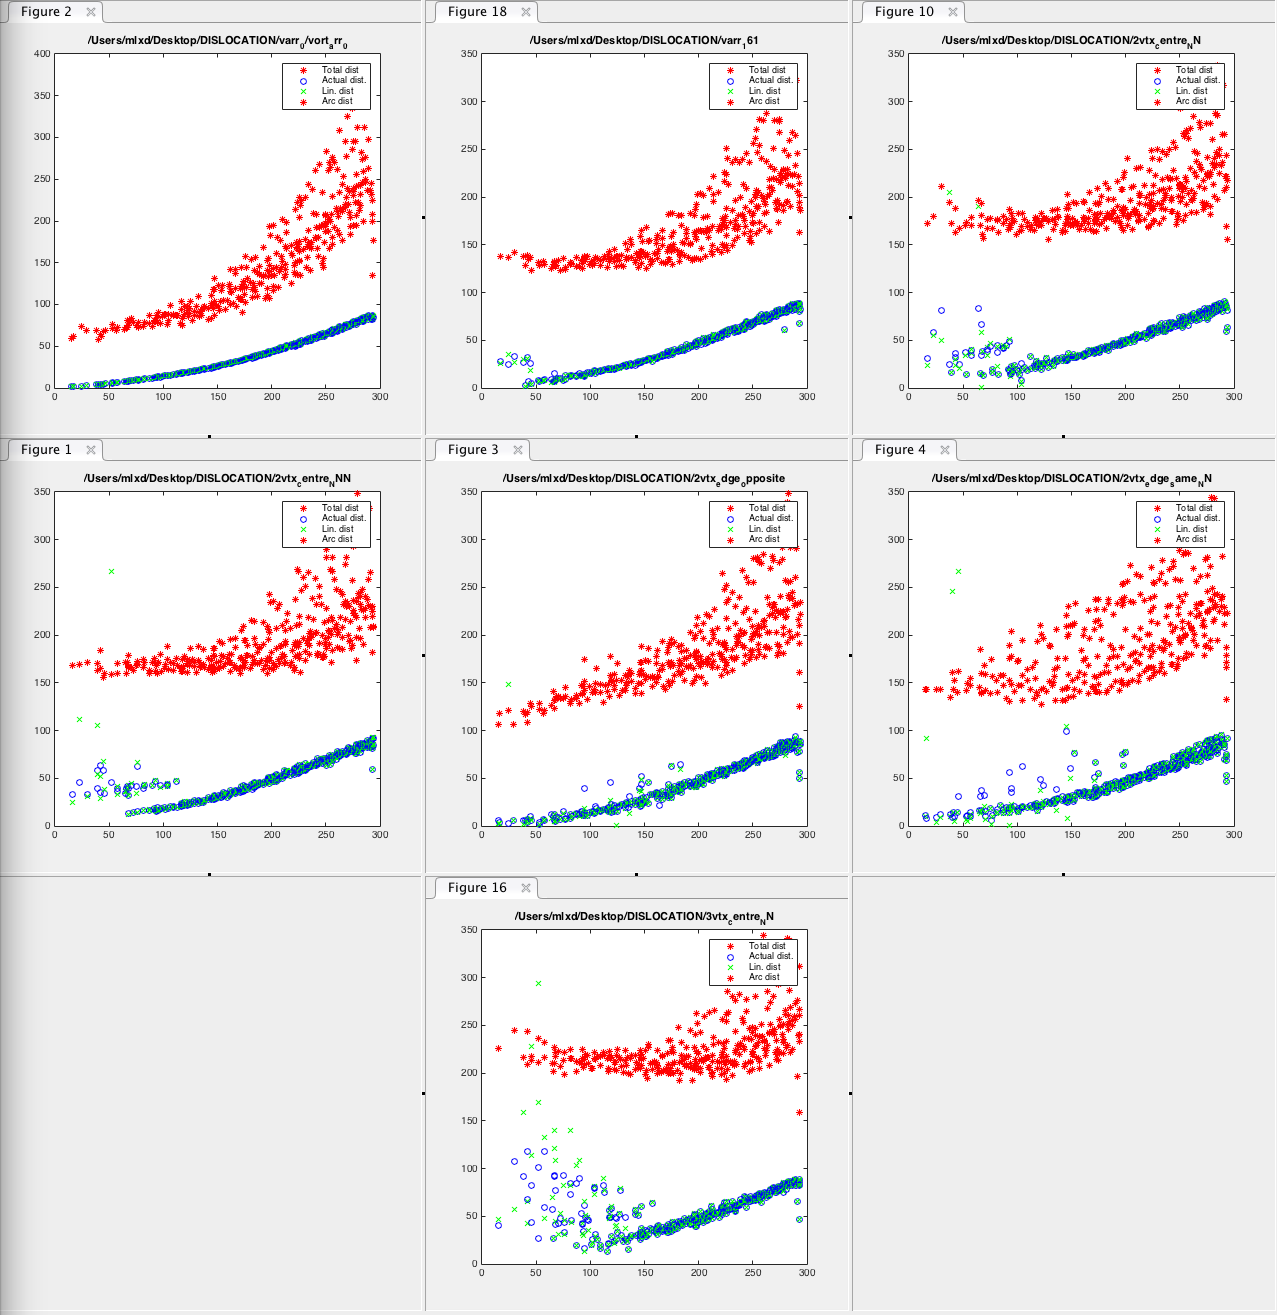
\includegraphics[width=0.48\textwidth]{imgs/vtx_distance_travelled}
	\caption{Vortex total traveled distance with different removal positions for between 1 and 3 vortices.}
	\label{fig:vtxdist}
\end{figure}
\fi



\subsubsection{Lattice overpopulation}
%%%%%%%%%%%%%%%%%%%%%%%%%%%%%%%%%%%%%%%%%%%%%%%%%%%%%%%%%%%%%%%%%%%%%%%%%%%%%%%%%%%%%%%%%%%%%%%%%%%%%%%%%%%%%%%%%%%%%%%%%%%%%%%%%%%%%%%%%%%%%
Similarly to removing a vortex from the lattice, we can also add one. By choosing a pre-existing vortex and adding a like-signed phase
winding, we can create multiply charged vortices in the condensate, where the vortex has a winding of $2\pi l$, with $l$ as the vortex
charge. Multiply charged vortices are usually unstable in condensates, as it is more energetically favourable to have two singly charged
vortices, than a single doubly charged vortex, as the energy increases with $l^2$. Thus, an $l$-charged vortex is expected to instead decay
into $l$ singly-charged vortices.

Here we have taken our lattice of $l=1$ vortices, and given an additional charge to a single vortex to examine the decay process. However,
the presence of the lattice suppresses the decay process for long times (order of seconds) compared to that of in a condensate without vortex
lattice. The doubly charged vortex remains stable on the order of seconds even away from the lattice centre (though does decay eventually).
The additional velocity profile locally causes the nearest neighbouring vortices to rotate faster than the solid-body rotation rate of the
whole lattice, causing a local shearing of the lattice structure. As with the vacancies, the use of correlation functions allowed us to
examine the short and long-range order of the lattice.

Voronoi diagrams of the resulting lattice show a stable doubly charged vortex position, with show twisting of the lattice about this central
point.

\begin{figure}[tb]
	\includegraphics[width=0.49\textwidth]{imgs/DoubleCharge/add161/voronoi}
	\includegraphics[width=0.49\textwidth]{imgs/DoubleCharge/add161remove207/voronoi}
	\caption{(top) Doubly charged central vortex. Doubly charged vortex remains stable, and retains 6-fold
	symmetry of vortex lattice. (bottom) Doubly charged central vortex, and removal of nearby vortex. Doubly charged vortex remains stable, and forms 8-fold
	symmetry of vortex neighbours.}
	\label{fig:voronoi_double}
\end{figure}



%%%%%%%%%%%%%%%%%%%%%%%%%%%%%%%%%%%%%%%%%%%%%%%%%%%%%%%%%%%%%%%%%%%%%%%%%%%%%%%%%%%%%%%%%%%%%%%%%%%%%%%%%%%%%%%%%%%%%%%%%%%%%%%%%%%%%%%%%%%%%
\subsection{Things to note}
%%%%%%%%%%%%%%%%%%%%%%%%%%%%%%%%%%%%%%%%%%%%%%%%%%%%%%%%%%%%%%%%%%%%%%%%%%%%%%%%%%%%%%%%%%%%%%%%%%%%%%%%%%%%%%%%%%%%%%%%%%%%%%%%%%%%%%%%%%%%%

\begin{itemize}
\item Localised disturbances: introducing vacancy to lattice causes it to travel with lattice. Change in velocity profile only affects 6
nearest neighbours on moderate timescales.
\item Long range hexatic phase has short range translational order (exp drop off), but constant orientational order -> is this such a phase?
\end{itemize}

%%%%%%%%%%%%%%%%%%%%%%%%%%%%%%%%%%%%%%%%%%%%%%%%%%%%%%%%%%%%%%%%%%%%%%%%%%%%%%%%%%%%%%%%%%%%%%%%%%%%%%%%%%%%%%%%%%%%%%%%%%%%%%%%%%%%%%%%%%%%%
\subsection{Correlations}
%%%%%%%%%%%%%%%%%%%%%%%%%%%%%%%%%%%%%%%%%%%%%%%%%%%%%%%%%%%%%%%%%%%%%%%%%%%%%%%%%%%%%%%%%%%%%%%%%%%%%%%%%%%%%%%%%%%%%%%%%%%%%%%%%%%%%%%%%%%%%
According to KTHNY theory for a 2D material the transition from a solid crystal to liquid phase is mediated through an intermediary hexatic
phase. This phase is usually characterised by the translational and orientational correlation functions. Given the lack of translation order
in a harmonically trapped condensate, we restrict our analysis to the orientational correlation function, $g_6$ given by
\iffalse
\begin{equation}
	\begin{aligned}
		g_6(|\mathbf{r}_i - \mathbf{r}_j|) &= \\ \frac{1}{N(r)}\displaystyle\sum_{i}^{N(r)}\displaystyle\sum_{j}^{N(r)} & \left(\frac{1}{n_j}\displaystyle\sum_{k}^{n_j}\exp(6\mathrm{i}\theta_{jk}) \right)\left(\frac{1}{n_i}\displaystyle\sum_{l}^{n_i}\exp(6\mathrm{i}\theta_{il}) \right)^{*}
	\end{aligned}
\end{equation}
\fi
\begin{equation}
	g_6(r) = \frac{1}{N(r)}\displaystyle\sum\limits_{i,j}^{N(r)}\psi_6(\mathbf{r}_i)\psi_6^{*}(\mathbf{r}_j),
\end{equation}
with
\begin{equation}
	\psi_6(|\mathbf{r}_{i} - \mathbf{r}_{j}|) = \frac{1}{n_i}\displaystyle\sum\limits_j^{n_i}\exp(6\mathrm{i}(\theta_i - \theta_j)),
\end{equation}
where $\psi_6$ is the orientational order parameter, and $j$ is over the nearest neighbouring vortices.

According to [] the decay in correlations for both translational and orientational order give indication to the material phase. In a
two-dimensional material the positional order is expected to decay algebraically as a function of radius, differing from that of a
three-dimensional material, which tends to a constant value. Here we examine the orientational correlation function as a measure of the
order of a "vortex unit cell", consisting of the angle made by nearest neighbours to an individual vortex. For a perfectly ordered
triangular lattice this value will tend to 1. To maintain constant vortex areal density, we choose vortices defined at a radius of
$r=2\times 10^4$ m from the centre, which give an almost uniform lattice constant for our system parameters.

\begin{itemize}
\item Crystalline: $\lim\limits_{r\rightarrow \infty}\hat{g}_T(r) \neq 0$, $\lim\limits_{r\rightarrow \infty}\hat{g}_6(r) \neq 0$
\item Long-range hexatic: $\hat{g}_T(r) \approx _{r\rightarrow \infty} \exp(-r/\xi_T) $, $\lim\limits_{r\rightarrow \infty}\hat{g}_6(r) \neq 0$
\item Power-law hexatic: $\hat{g}_T(r) \approx _{r\rightarrow \infty} \exp(-r/\xi_T) $, $\hat{g}_6(r) \approx _{r\rightarrow \infty} 1/r^{\eta_6}$
\item Amorphous: $\hat{g}_T(r) \approx _{r\rightarrow \infty} \exp(-r/\xi_T) $, $\hat{g}_6(r) \approx _{r\rightarrow \infty} \exp(-r/\xi_6) $
\end{itemize}
Hat means normalised (see page 119 of order in two dim binary random arrays, Nelson et al.)


%%%%%%%%%%%%%%%%%%%%%%%%%%%%%%%%%%%%%%%%%%%%%%%%%%%%%%%%%%%%%%%%%%%%%%%%%%%%%%%%%%%%%%%%%%%%%%%%%%%%%%%%%%%%%%%%%%%%%%%%%%%%%%%%%%%%%%%%%%%%%
\subsection{Numerics and results}\label{sec:numerics}
%%%%%%%%%%%%%%%%%%%%%%%%%%%%%%%%%%%%%%%%%%%%%%%%%%%%%%%%%%%%%%%%%%%%%%%%%%%%%%%%%%%%%%%%%%%%%%%%%%%%%%%%%%%%%%%%%%%%%%%%%%%%%%%%%%%%%%%%%%%%%

Each vortex position was found by summing over adjacent grid sites, and looking for a $2\pi$ phase winding. This gave a vortex position
estimated to the numerical grid. A least-squares fit was performed to more accurately determine the vortex core. Vortices closest the centre
of the condensate were considered to ensure an almost uniform inter-vortex spacing, giving minimal deviation in lattice constant, $a_0$. Each
vortex was assigned a unique identifier (UID) to allow for it to be tracked individually over the course of the simulations, with the initial
configuration presented in the graph [ref graph]. By noting these UIDs, vortices can be individually selected for removal by applying the
global $2\pi$ phase winding in the opposing direction, centered on the core.

The trajectory plots show very small global effect on the core positions, with a disturbance localised in a region centered on the removed
core. By removing vortices in different locations on the condensate we see similar behaviour, with the trajectories modified in a region
around the removed vortex. The removal of two vortex adjacent cores can be seen to crate a greater disturbance, as expected, with the
trajectories of the surrounding vortices no longer following an almost circular path (more like hexagonal), but taking on other geometric
path shapes. For two nn vortices the path becomes an almost rhombic shape, with nnn forming an elongated hexagon (as to be expected). For 3
nn, the resulting trajectories follow a triangular pattern of the same orientation as the removed vortices. For the removal of an entire 7
vortex cell, the formed pattern is star shaped.

TODO:
Calculate incompressible kinetic energy spectrum for each case, and see if useful. RESULT: It wasn't.
Calculate $S(k) = |\Psi(k)|^2$ for condensate densities, not just vortex positions, for comparison. RESULT: looks strange, even in untouched
case. Arcs exist in all cases, but with interference lines.

The impact on the overall distances traveled by each vortex as a result of the dislocations is given in figure [some fig].

\iffalse
\begin{figure}[tb]
	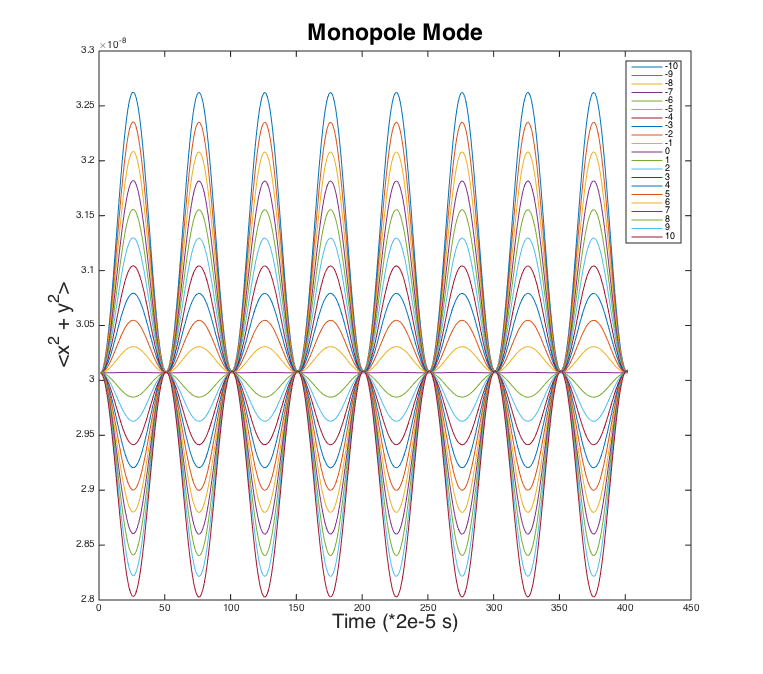
\includegraphics[width=0.48\textwidth]{imgs/mono}
	\caption{The oscillation of the mean-radius of the condensate after the addition of vortices (positive) or antivortices (negative) with
	different imprinted windings. The oscillation mode shows an exact match for a 2D non-rotating condensate of $2\omega_{\perp}$ for all cases.}
\end{figure}
fi

\begin{figure}[tb]
	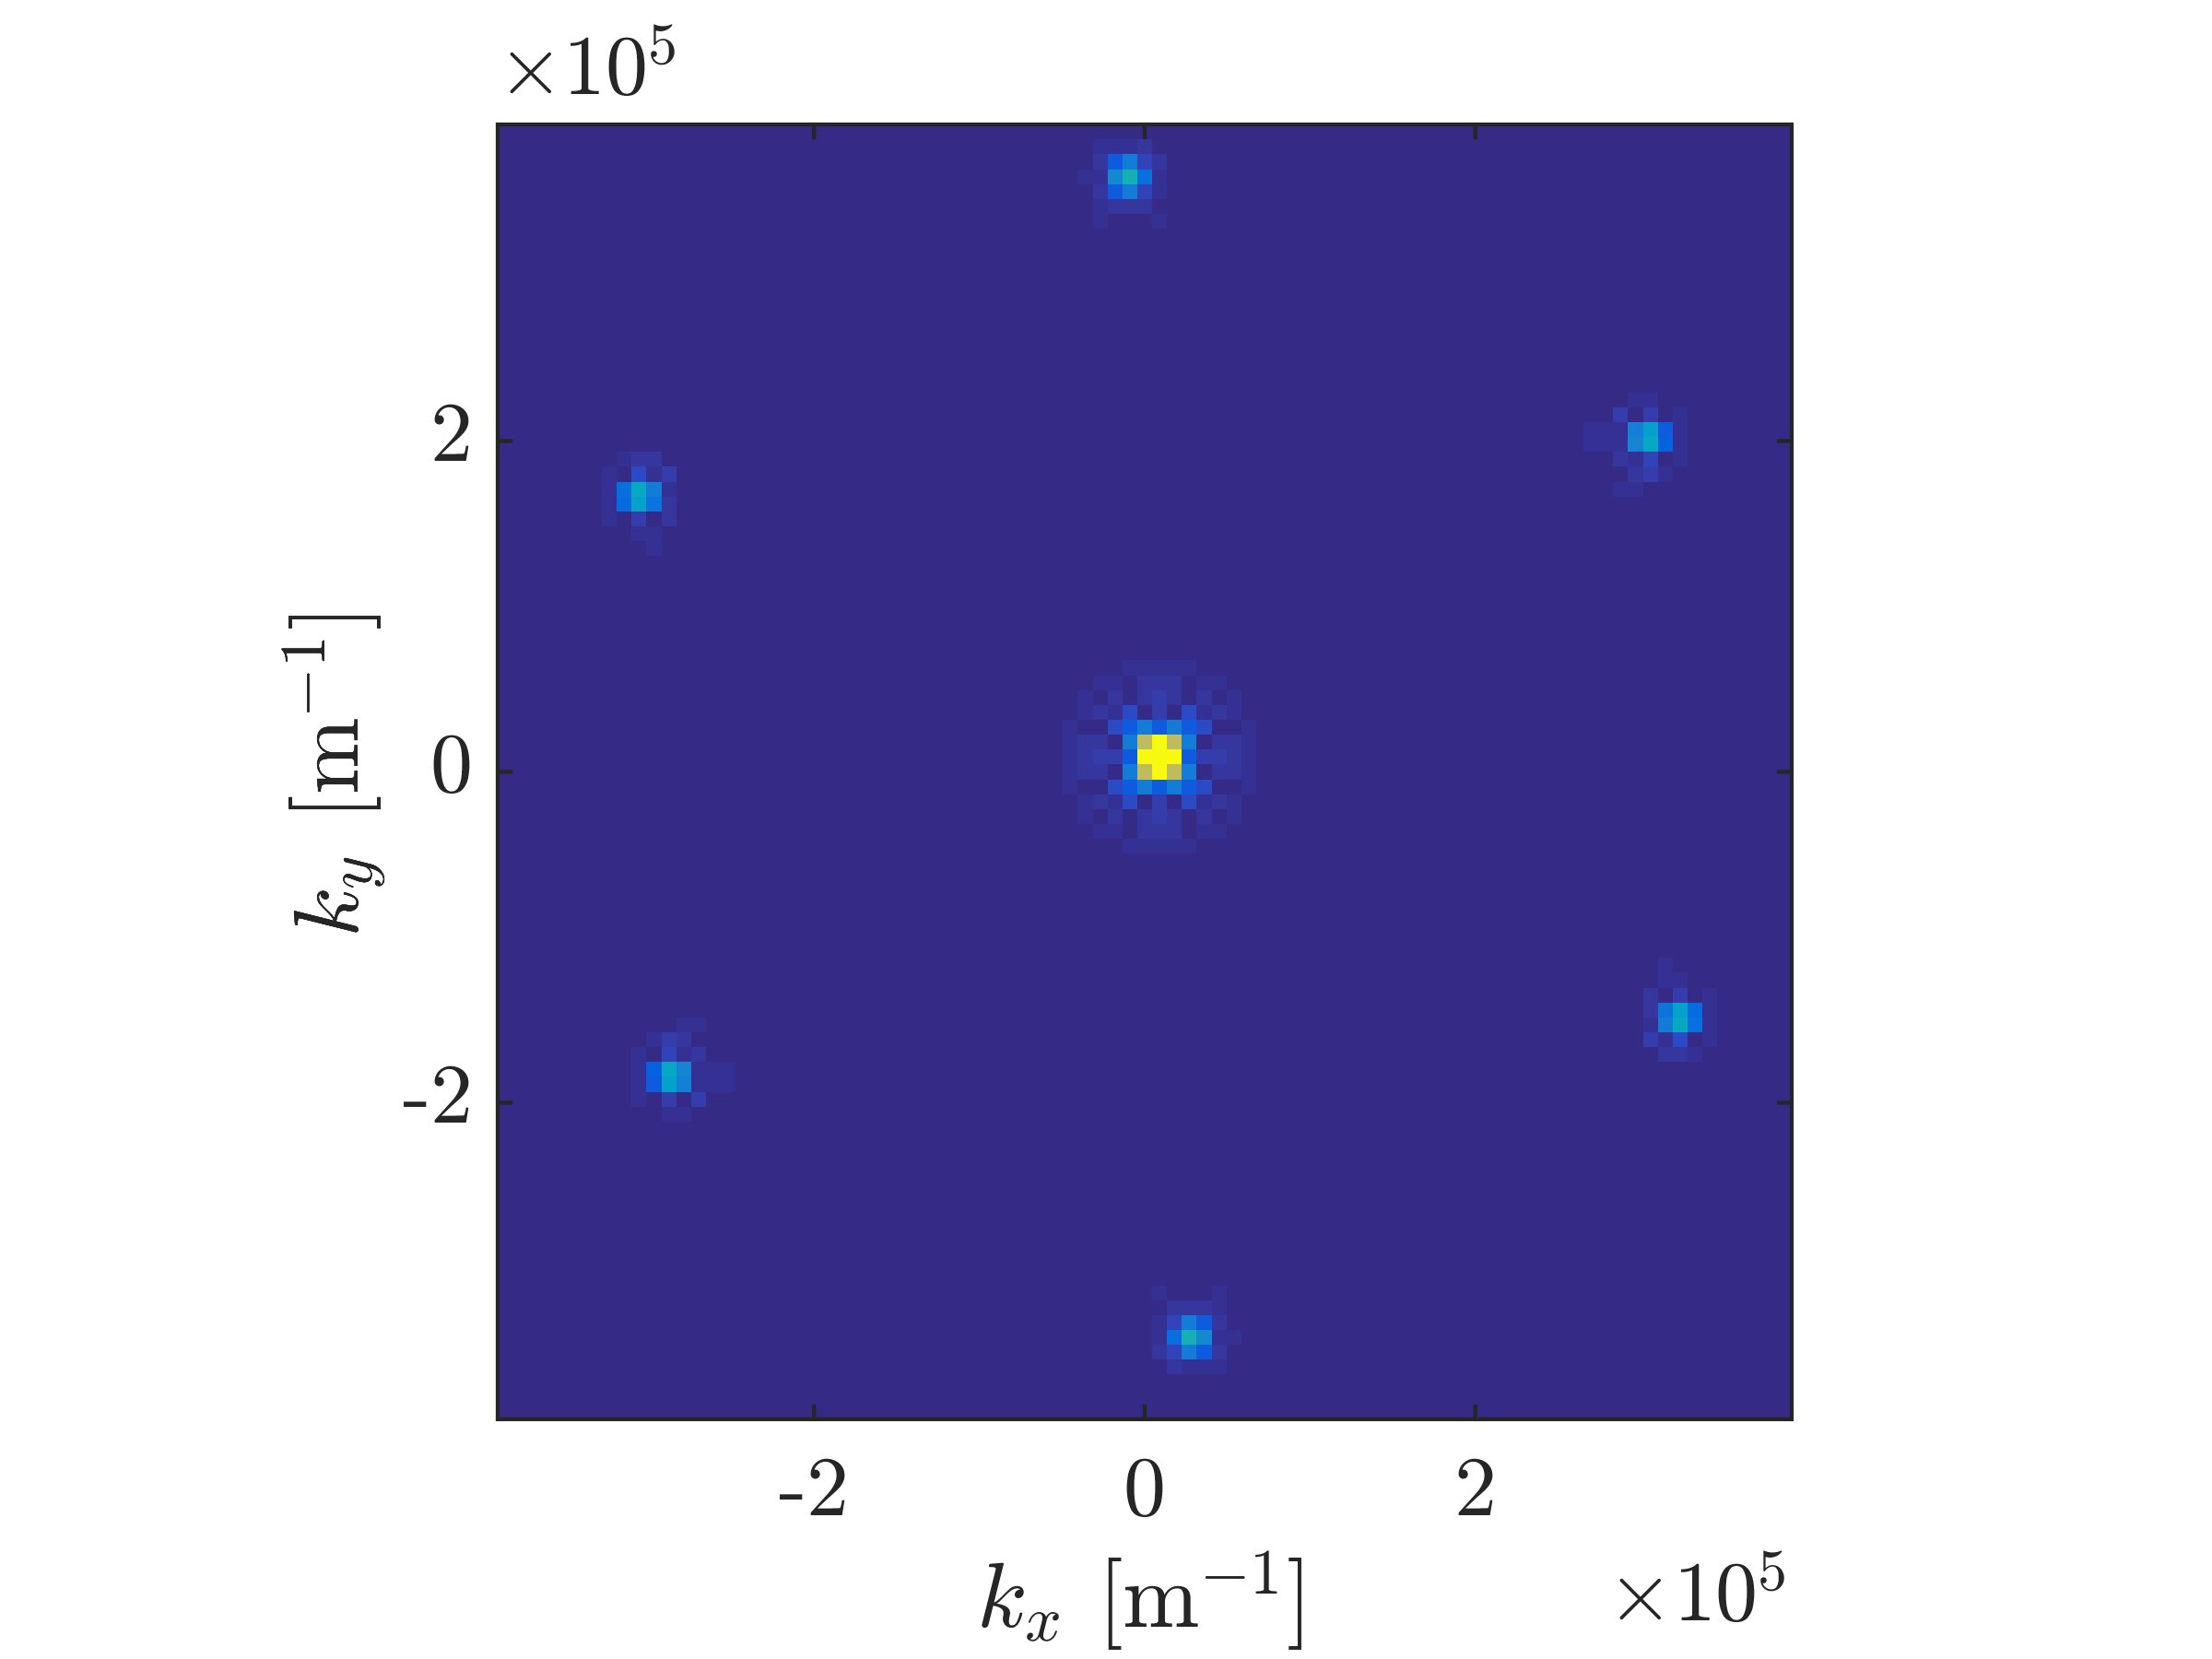
\includegraphics[width=0.48\textwidth]{imgs/FFT_density_linear_cell}
	\caption{Density structure factor within 4*pi/(sqrt(3)*d0).}
\end{figure}

%\begin{figure}[h!]
%	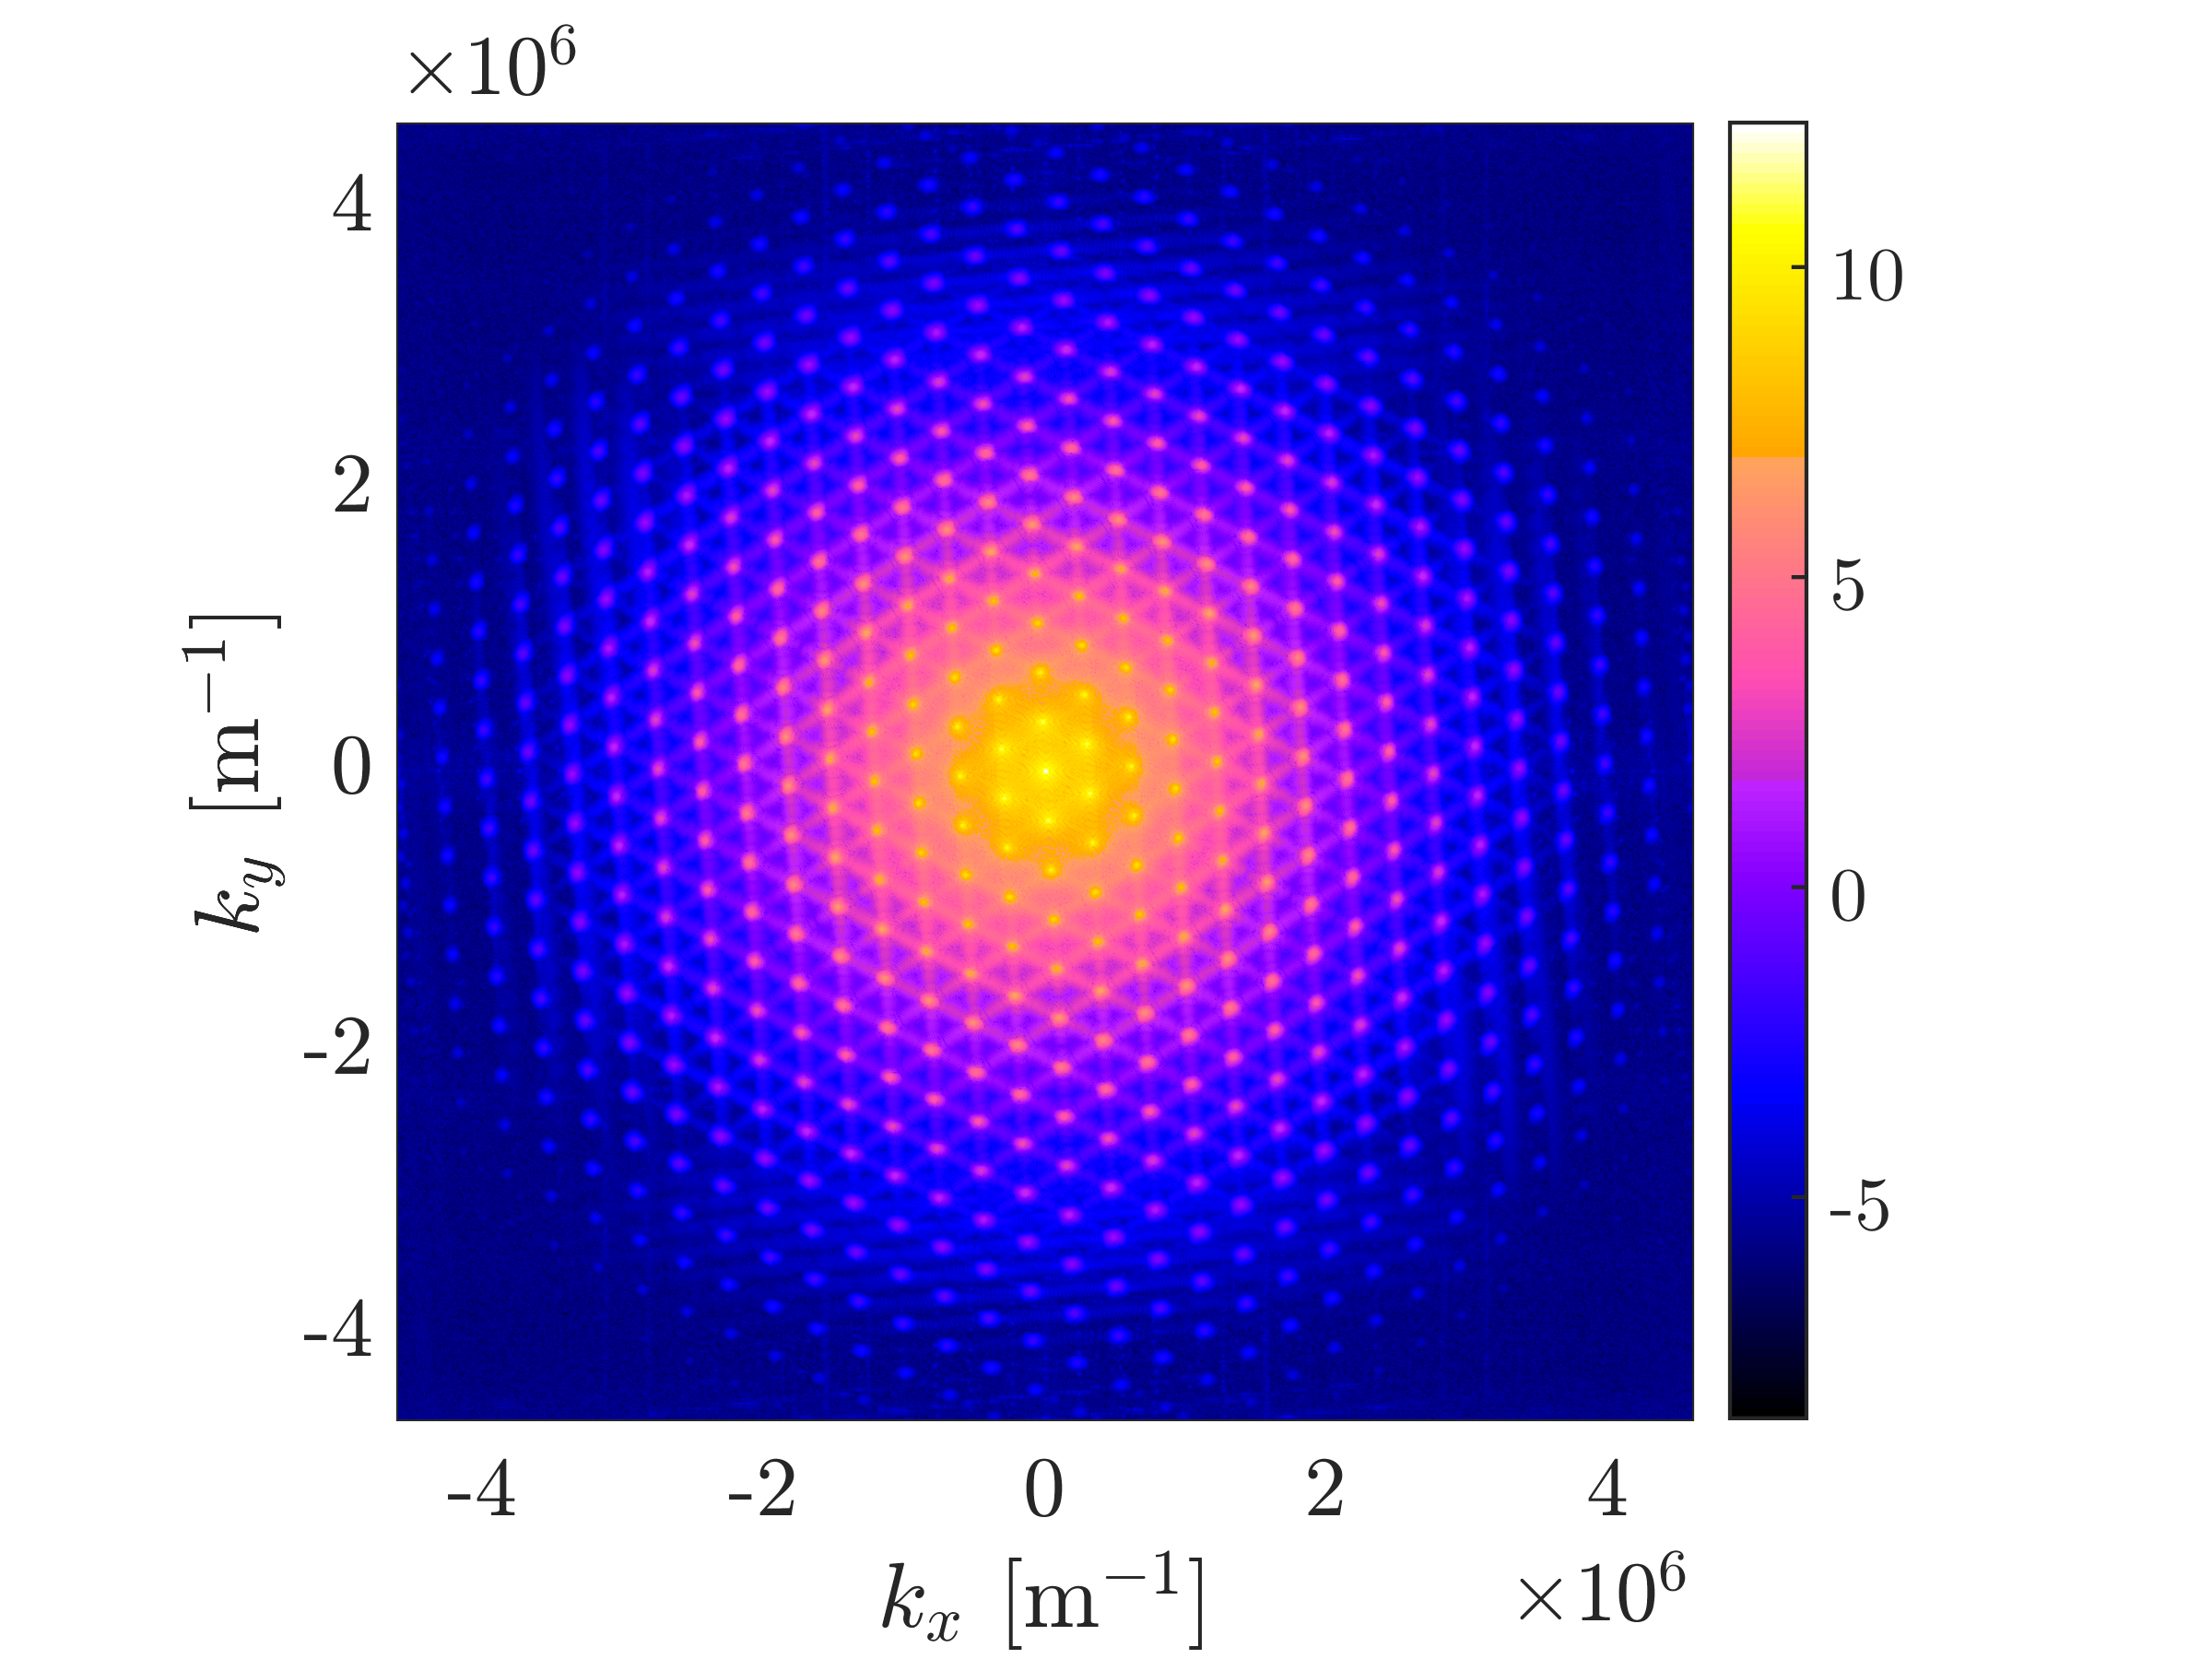
\includegraphics[width=0.48\textwidth]{imgs/FFT_density}
%	\caption{Density structure factor.}
%\end{figure}

\begin{figure}[tb]
	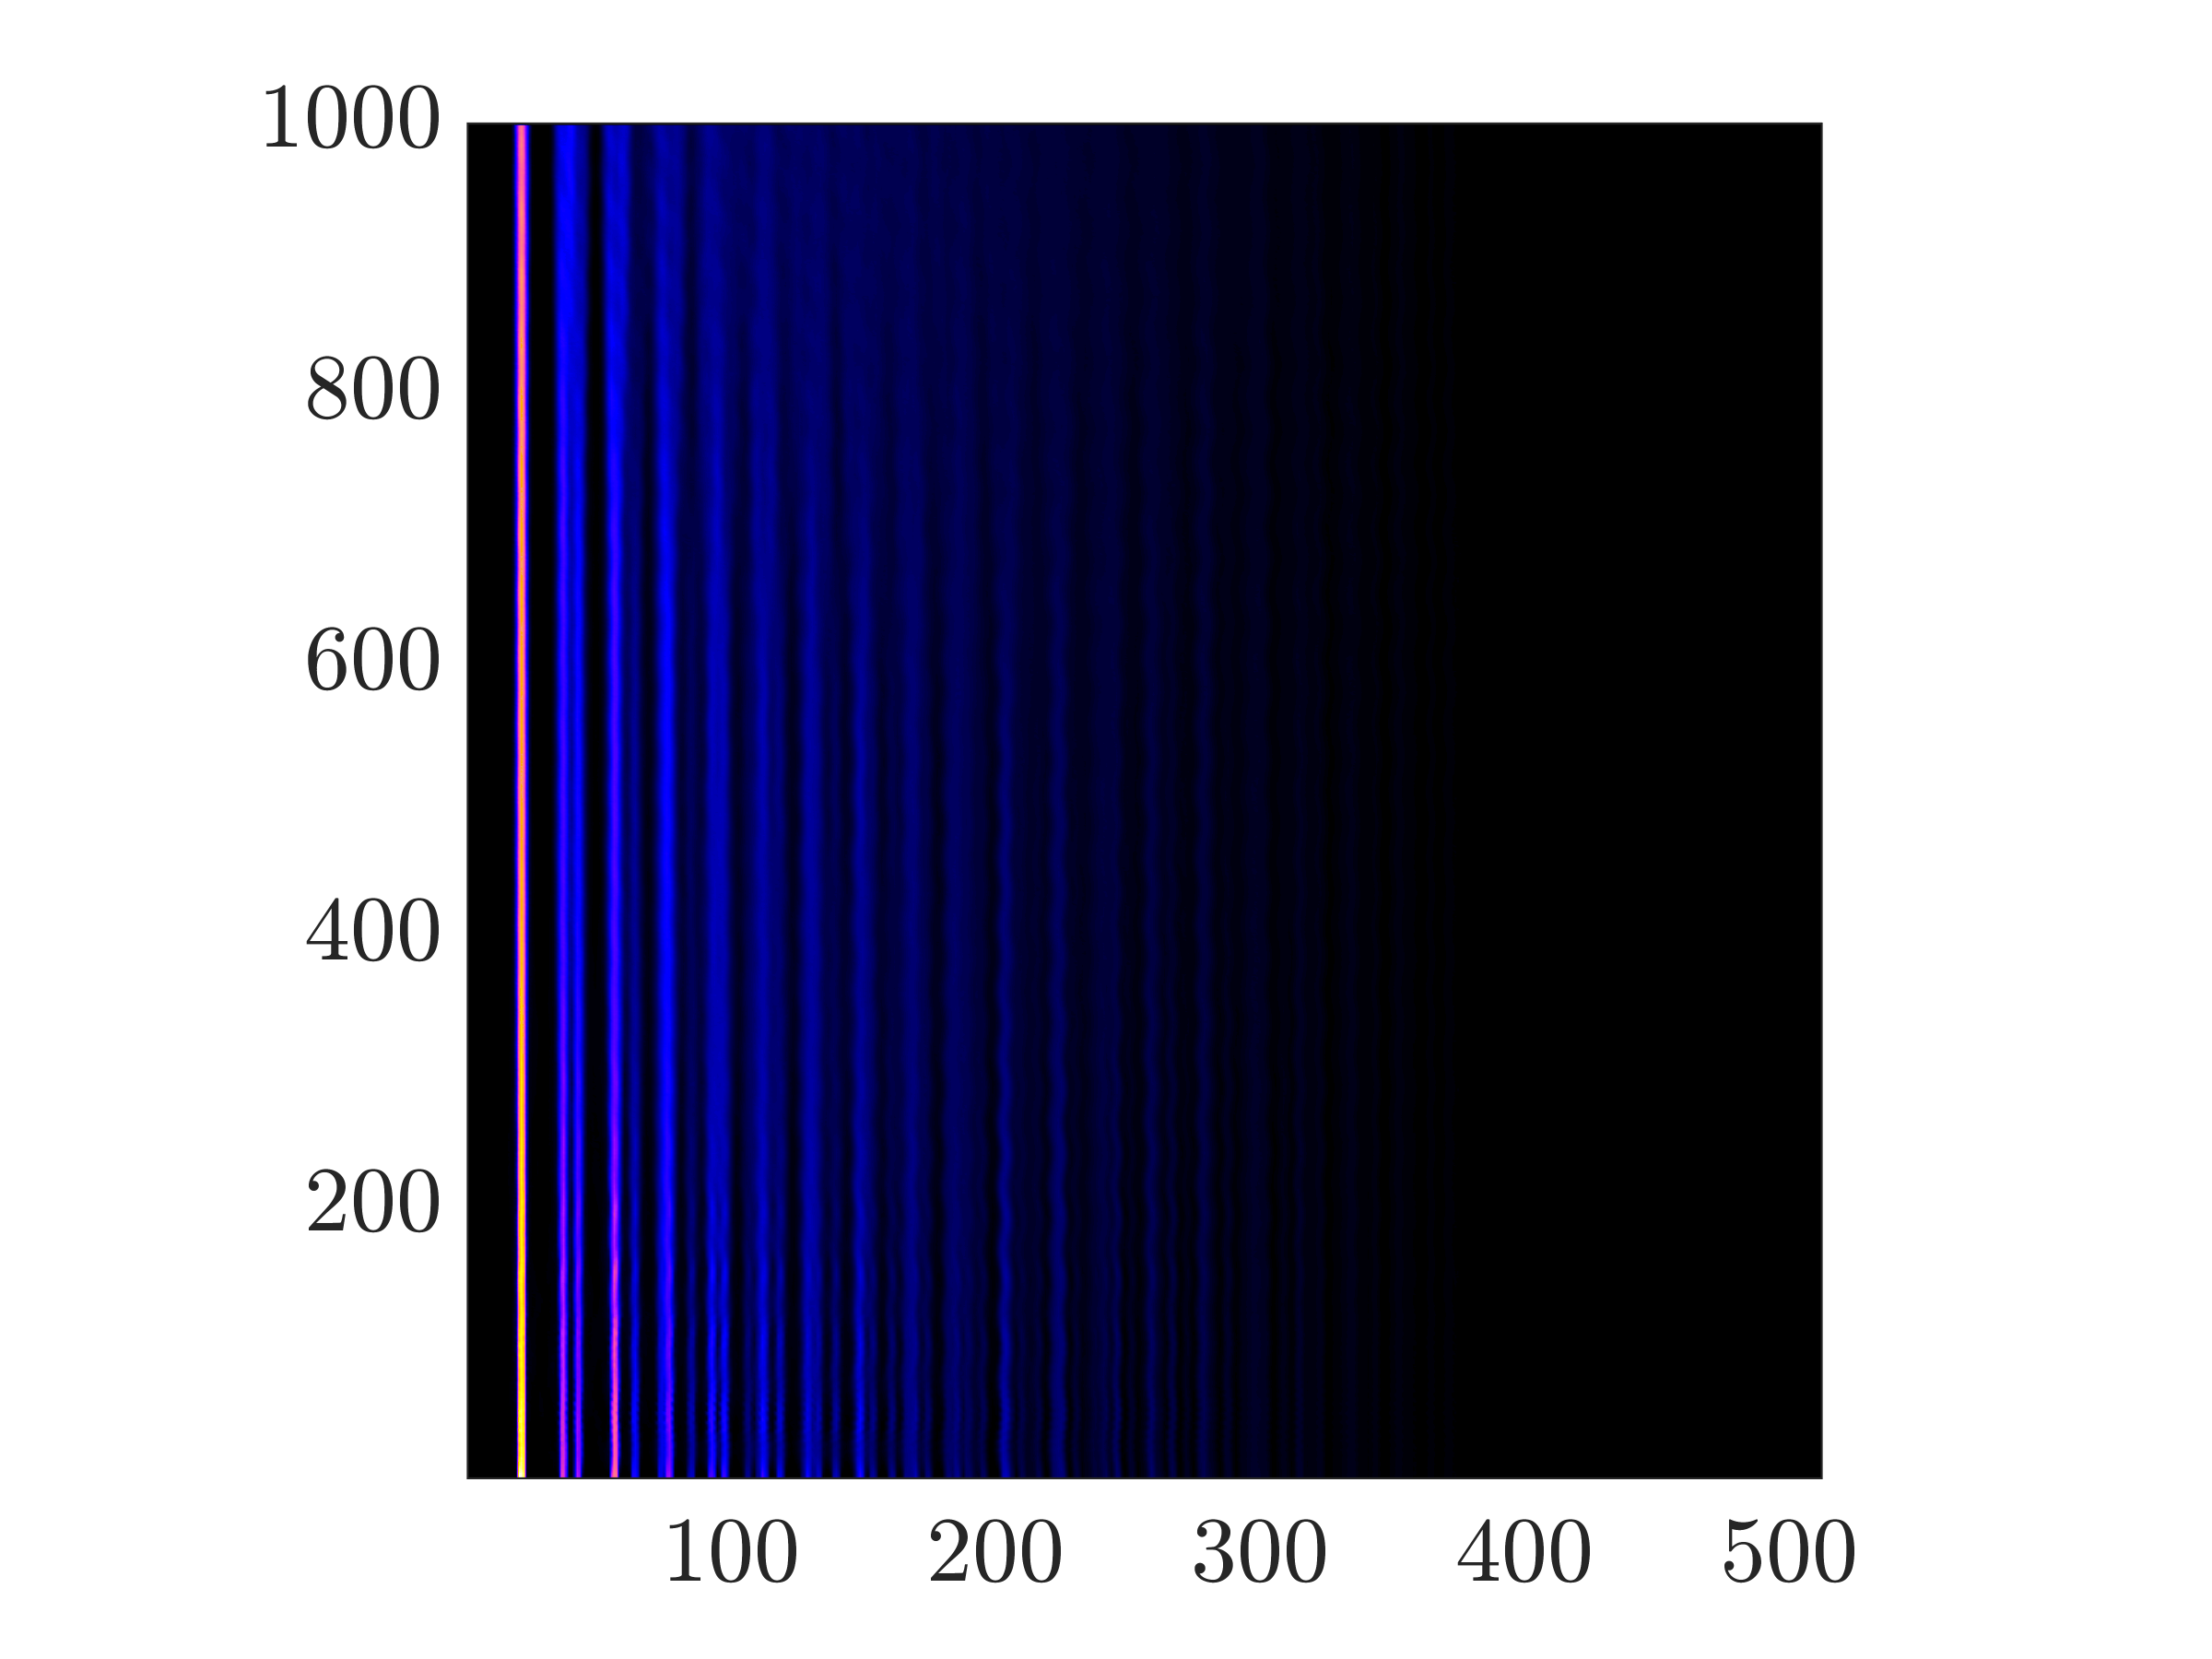
\includegraphics[width=0.48\textwidth]{imgs/RDF_time_gp}
	\caption{Radial distribution function over time after removing vortex from lattice centre. }
\end{figure}


\begin{figure}[tb]
	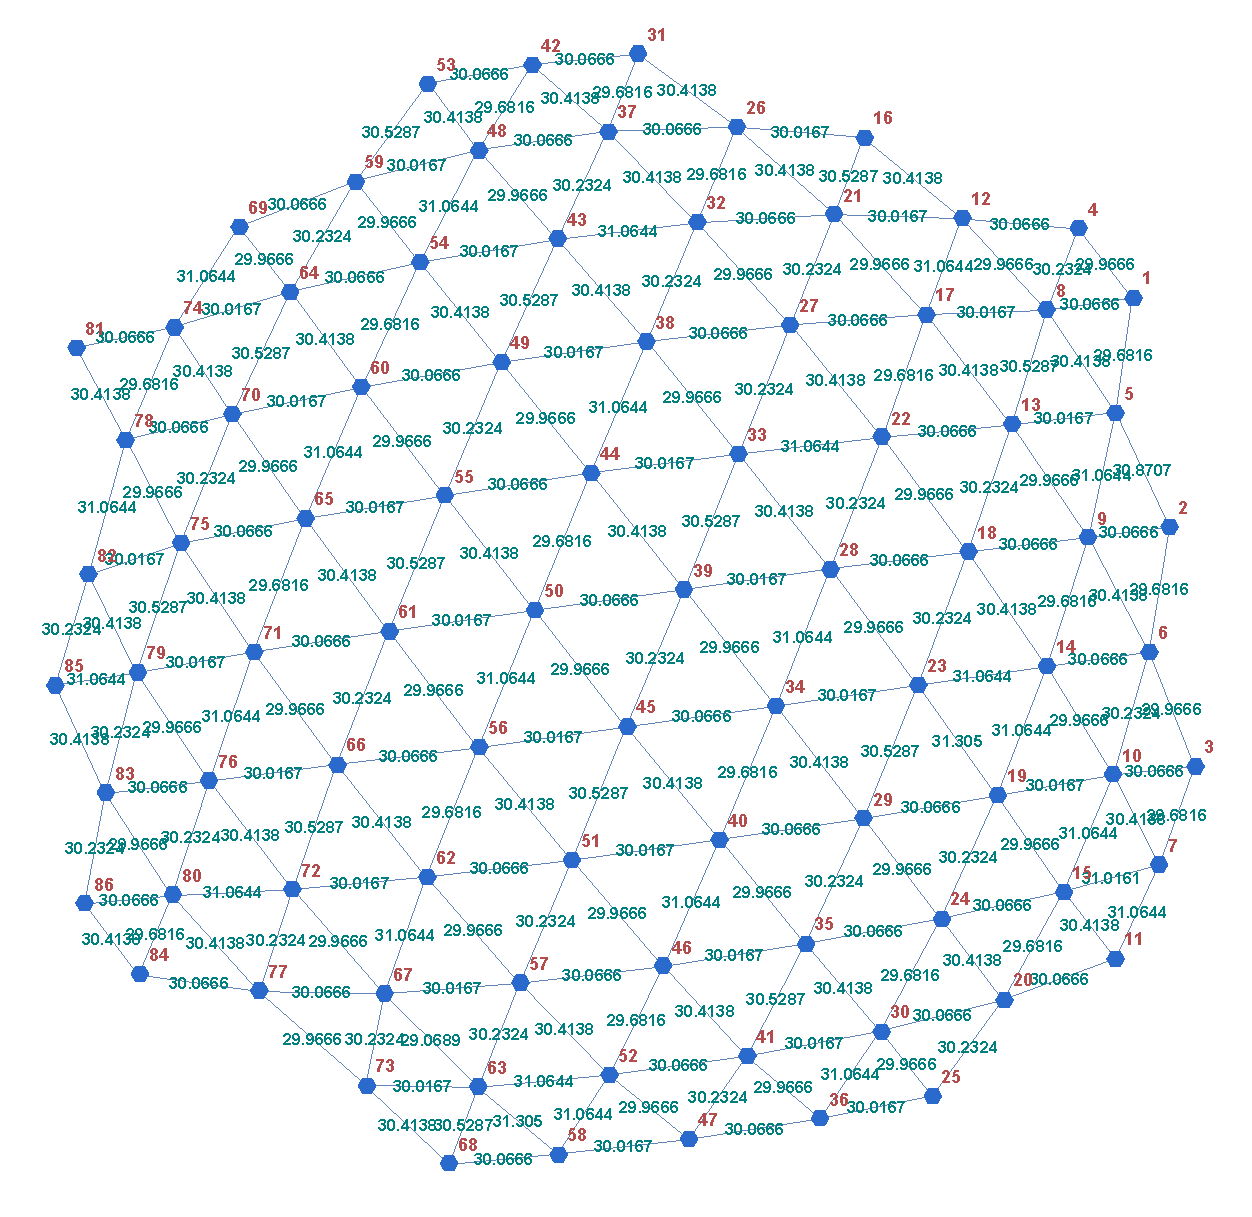
\includegraphics[width=0.48\textwidth]{imgs/graph86}
	\caption{Condensates vortices treated as nodes in a graph. Edges are drawn between nearest neighbours.}
\end{figure}
%\fi
%%%%%%%%%%%%%%%%%%%%%%%%%%%%%%%%%%%%%%%%%%%%%%%%%%%%%%%%%%%%%%%%%%%%%%%%%%%%%%%%%%%%%%%%%%%%%%%%%%%%%%%%%%%%%%%%%%%%%%%%%%%%%%%%%%%%%%%%%%%%%
\section{Conclusions}\label{sec:conc}
%%%%%%%%%%%%%%%%%%%%%%%%%%%%%%%%%%%%%%%%%%%%%%%%%%%%%%%%%%%%%%%%%%%%%%%%%%%%%%%%%%%%%%%%%%%%%%%%%%%%%%%%%%%%%%%%%%%%%%%%%%%%%%%%%%%%%%%%%%%%%

The removal of a vortex from the lattice creates a stable vacancy site, which in the corotating frame, travels with the lattice for some time
before decaying into paired 5 and 7 nearest neighbour disclinations. These disclination pairs can be viewed as as an edge dislocation in the
lattice. The resulting grain boundary breaks the 6-fold symmetry of the triangular lattice. The removal of the single vortex also removes the
velocity profile associated with the vortex at that location. The local velocity near the vacancy will be less than the solid-body behaviour
of the lattice. This causes the nearest neighbour vortices to rotate slower than the condensate, locally creating a strain/shear? on the
lattice. Local competition to fill the vacancy ensures its long-lived stability. The removal of the central vortex creates a local honeycomb
lattice structure, which according to [stat top of 2d lattice] will decay (following perturbation) via three possible processes.

Increasing the charge of a vortex by applying the same signed phase winding to a vortex core creates a stable doubly charged vortex for long
times (seconds). This, like the stable vacancy, seems to be stable at any range of positions (but decays faster at outskirts). The additional
velocity field shears the lattice, with the resulting correlations showing long-range power-law behaviour. This is usually indicative of a
power-law hexatic phase. Given the lack of true translational order in a harmonically trapped vortex lattice, it remains more instructive to
investigate the static structure factor of the system. The hexatic phase is expected to show spreading of the Fourier peaks into arcs. Here,
though we see such spreading, it is not entirely arc-like, and does not match entirely with the expectations of a hexatic phase.	



%%%%%%%%%%%%%%%%%%%%%%%%%%%%%%%%%%%%%%%%%%%%%%%%%%%%%%%%%%%%%%%%%%%%%%%%%%%%%%%%%%

\fi
%%%%%%%%%%%%%%%%%%%%%%%%%%%%%%%%%%%%%%

% Unnumbered chapters (for example conclusion) - Comment if unnecessary
\newif\ifconc
\unnumberedchapter{Conclusion} % Title of the unnumbered chapter
\chapter*{Conclusion}  % Name of the unnumbered section

This is the conclusion. You might want to leave it unnumbered, as it is now. If you want to number it, treat it like any other chapter.% Conclusion (unnumbered)

%----------------------------------------------------------------------------------------
%	APPENDICES
%----------------------------------------------------------------------------------------

\addtocontents{toc}{\vspace{2em}} % Add a gap in the Contents, for aesthetics
\appendix % Starts of appendices

\numberedchapter


\chapter{Appendices and Supplementary Data} \label{appA}

Unlike a journal article, no data or discussion may be presented separately as unpublished supplementary documents or data.  Appendices should be used instead for material that is tangentially relevant to the thesis but does not fit in the main narrative. If you need to refer to large volumes of data that cannot be printed (such as an annotated genome, or a simulation with moving images), lodge the data on an OIST repository or a public database and provide the URL of the dataset in the thesis.  

%\input{MainText/appendixB}
%\input{MainText/appendixC}

%----------------------------------------------------------------------------------------
%	BIBLIOGRAPHY
%----------------------------------------------------------------------------------------

\addtocontents{toc}{\vspace{2em}} % Add a gap in the Contents, for aesthetics
\unnumberedchapter{Bibliography} % Title of the unnumbered chapter
\bibliography{Preamble/MLXD_LIB} % The references information are stored in the file named "Thesis_bibliography.bib"


\end{document}
